\documentclass[a4paper,11pt]{article}
\usepackage[english]{babel}
\usepackage[utf8]{inputenc}
% package for including graphics with figure-environment
\usepackage{graphicx}
\usepackage{float}
\usepackage{dirtree}
\usepackage[backend=biber,natbib=true,style=numeric,sorting=none]{biblatex}
\addbibresource{references.bib}
% Enhanced hyperref setup with professional colors
\usepackage{hyperref}
\hypersetup{
    colorlinks=true,
    linkcolor=blue!80!black,      % Internal links (TOC, references)
    citecolor=blue!70!black,      % Citation links
    filecolor=magenta!60!black,   % File links
    urlcolor=blue!60!black,       % URL links
    bookmarksnumbered=true,
    bookmarksopen=true,
    bookmarksopenlevel=1,
    pdfstartview=FitH,
    pdftitle={Multimodal Trajectory Prediction in Multi-Agent Scenarios},
    pdfauthor={Jan Duchscherer, Lukas Röß},
    pdfsubject={Seminar: Video Analysis and Object Detection},
    pdfkeywords={trajectory prediction, multi-agent, video analysis, query-centric, deep learning}
}

% Suppress citation warnings - temporarily disable warnings for citations and references
\usepackage{silence}
\WarningFilter{latex}{Citation}
\WarningFilter{latex}{Reference}
\WarningFilter{natbib}{Citation}

% Enhanced mathematical typesetting
\usepackage{amsmath,amssymb,amsthm}  % Core mathematical packages
\usepackage{mathtools}               % Enhanced math tools and fixes
\usepackage{bbm}                     % For blackboard bold symbols (\mathbbm)
\usepackage{dsfont}                  % Alternative for blackboard bold
\usepackage{bm}                      % Bold math symbols
% Enhanced code listings and algorithms
\usepackage{enumitem}
\usepackage{listings}         % For code listings
\usepackage{algorithm}        % For algorithm environments
\usepackage{algorithmic}      % For algorithmic pseudo-code
\usepackage{xcolor}           % For colored text (needed for \definecolor)

% Professional code styling
\definecolor{codegreen}{rgb}{0,0.6,0}
\definecolor{codegray}{rgb}{0.5,0.5,0.5}
\definecolor{codepurple}{rgb}{0.58,0,0.82}
\definecolor{backcolour}{rgb}{0.95,0.95,0.92}

\lstdefinestyle{mystyle}{
    backgroundcolor=\color{backcolour},
    commentstyle=\color{codegreen},
    keywordstyle=\color{magenta},
    numberstyle=\tiny\color{codegray},
    stringstyle=\color{codepurple},
    basicstyle=\ttfamily\footnotesize,
    breakatwhitespace=false,
    breaklines=true,
    captionpos=b,
    keepspaces=true,
    numbers=left,
    numbersep=5pt,
    showspaces=false,
    showstringspaces=false,
    showtabs=false,
    tabsize=2,
    frame=single,
    rulecolor=\color{blue!30!black}
}
\lstset{style=mystyle}

% Enhanced algorithm formatting
\renewcommand{\algorithmicrequire}{\textbf{Input:}}
\renewcommand{\algorithmicensure}{\textbf{Output:}}
\renewcommand{\algorithmiccomment}[1]{\hfill\textcolor{blue!60!black}{\textit{#1}}}
\usepackage{tikz}             % For vector graphics and diagrams
\usepackage{pgfplots}         % For plotting graphs and data visualization
\usepackage{subcaption}       % For subfigures and subcaptions
\usepackage{booktabs}         % For better looking tables
\usepackage{tabularx}
\usepackage{adjustbox}
\usepackage{siunitx}
\usepackage{longtable}        % For tables spanning multiple pages
\usepackage{microtype}        % For better typography
\usepackage{array}            % Enhanced table column types
\usepackage{multirow}         % Multi-row table cells
\usepackage{rotating}         % Rotating tables and figures
\usepackage{caption}          % Enhanced captions
\usepackage{csquotes}         % For proper quotations
\usepackage{enumitem}         % Enhanced lists
\usepackage{parskip}          % Better paragraph spacing
\usepackage{dirtree}
% \usepackage{geometry}         % Page layout and margins
% Professional caption formatting

% Enhanced table row colors
\definecolor{lightgray}{rgb}{0.9,0.9,0.9}
\definecolor{lightblue}{rgb}{0.9,0.95,1.0}

% Custom commands and mathematical notation
\newcommand{\SE}[1]{\mathrm{SE}(#1)}  % Special Euclidean group
\newcommand{\R}{\mathbb{R}}            % Real numbers
\newcommand{\N}{\mathbb{N}}            % Natural numbers
\newcommand{\Z}{\mathbb{Z}}            % Integers
\newcommand{\C}{\mathbb{C}}            % Complex numbers
\newcommand{\norm}[1]{\left\|#1\right\|}  % Norm
\newcommand{\abs}[1]{\left|#1\right|}     % Absolute value
\newcommand{\argmin}{\operatorname{argmin}}
\newcommand{\argmax}{\operatorname{argmax}}

% Custom symbols for pros/cons lists
\newcommand{\greenoplus}{\textcolor{green!70!black}{\(\oplus\)}}
\newcommand{\redominus}{\textcolor{red!70!black}{\(\ominus\)}}
\newcolumntype{Y}{>{\ttfamily\arraybackslash}X}


% Enhanced TikZ and PGFPlots settings
\usetikzlibrary{arrows.meta, positioning, shapes.geometric, decorations.pathreplacing, calc, backgrounds, angles, quotes}
\pgfplotsset{
    compat=1.18,
    width=10cm,
    height=6cm,
    grid=major,
    grid style={dashed,gray!30},
    axis line style={blue!60!black},
    tick style={blue!60!black},
    label style={blue!80!black},
    legend style={blue!80!black}
}

% Enhanced footnote styling
\usepackage[hang,flushmargin]{footmisc}
\renewcommand{\footnotelayout}{\color{blue!60!black}\footnotesize}

% Enhanced list formatting
\setlist[enumerate]{leftmargin=*,labelsep=0.5em}
\setlist[itemize]{leftmargin=*,labelsep=0.5em}
\setlist[description]{leftmargin=*,labelsep=0.5em}

% package for bibliography
% Enhanced headers and footers
\usepackage{fancyhdr}

\pagestyle{fancy}
\fancyhf{} % clear all header and footer fields
\fancyhead[L]{Jan Duchscherer, Lukas Röß}
\fancyhead[R]{\today}
    \fancyfoot[C]{\thepage}
    \renewcommand{\headrulewidth}{0.3pt}
\setlength{\headheight}{15pt}

% Enhanced section styling for article class
\usepackage{titlesec}
\titleformat{\section}
  {\normalfont\Large\bfseries\color{blue!80!black}}
  {\thesection}{1em}{}
\titlespacing*{\section}{0pt}{20pt}{15pt}

\titleformat{\subsection}
  {\normalfont\large\bfseries\color{blue!70!black}}
  {\thesubsection}{1em}{}
\titleformat{\subsubsection}
  {\normalfont\normalsize\bfseries\color{blue!60!black}}
  {}{0em}{}

\newcommand{\subsubsubsection}[1]{\paragraph{#1}\mbox{}\\}

\begin{document}
	\title{
	\begin{figure}[!ht]
	\centering
			
\includegraphics[width=0.7\textwidth]{figures/hm-logo.pdf}
	\end{figure}
	\vspace{1cm}
	\Huge Multimodal Trajectory \\ Prediction in Multi-Agent Scenarios \\
	}

    \vspace{1cm}

	% Insert here your name and correct mail address
	\author{\Large \href{mailto:jan.duscherer@hm.edu}{Jan Duscherer} \and \Large \href{mailto:lukas.roess@hm.edu}{Lukas Röß}
	\vspace{1cm}}

	% name of the course and module
	\date{
	\large Seminar: Video Analysis and Object Detection \\
	\vspace{0.8cm}
	\large Lecturer: Prof. Dr. Claudius Schnörr \\
	\vspace{1cm}
	\today
	}

	\maketitle
	\setlength{\parindent}{0pt}

\newpage
% Enhanced table of contents
\tableofcontents
\clearpage

\listoffigures
\clearpage

\listoftables
\clearpage

%%%%% Include chapters as sections %%%%%

\section{Introduction}
\label{sect:introduction}

\subsection{The Autonomous Driving Stack}
Safe and efficient navigation in autonomous driving hinges on a multi-stage pipeline of \emph{perception}, \emph{prediction}, \emph{ego-planning} and \emph{control} \cite{hu2023planning}. The perception module processes raw sensor streams such as LiDAR, radar, and multi-view camera data to produce a rich representation of the scene, including the (kinematic) states of all traffic participants (\emph{agents}, i.e., vehicles, pedestrians, cyclists) and static map elements like lane markings, traffic lights and pedestrian crossings \cite{lmformerYadav2025}.
This vectorized scene-representation serves as the input to the \emph{motion forecasting} module, which is tasked with inferring the future trajectories of all agents in the scene over some planning horizon. The output is not a single, deterministic path, but a probabilistic, multimodal distribution over possible futures of each agent, which enables the pro-active planning of feasible and safe maneuvers and ego-trajectories from which the control module can derive the necessary vehicle commands.

\subsection{Challenges in Multi-Agent Motion Forecasting}
Despite impressive advances, three interrelated challenges limit current motion forecasting models
The behavior of traffic participants is inherently \emph{non-deterministic} and involves highly complex interactions with the environment and other agents. This necessitates models that can capture these complex dynamics and produce diverse, probabilistic motion forecasts to account for the wide range of possible future behaviors, whose uncertainty grows exponentially with the planning horizon as errors compound over time.
Attention-based architectures have emerged as powerful tools to model these complex interactions and overcome the issue of \emph{mode collapse} that plagued earlier approaches. However, traditional \emph{agent-centric} encoding schemes require expensive per-frame re-normalization, preventing the caching and reuse of previously computed features and hindering real-time performance\cite{qcnextZhou2023}.
Third, \emph{scalability and generalization} remain elusive: models trained on a single dataset like nuScenes, Argoverse 2, and Waymo \cite{caesar2020nuscenes, av2Wilson2023, wmodSun2020} often fail to transfer across benchmarks with disparate formats, sampling rates, and map semantics \cite{unitrajFeng2024}.

\subsection{Contributions and Report Structure}
In this report, we explore these challenges by unifying data, theory, and models within the \texttt{UniTraj} framework.

We begin in Section~\ref{sec:background} by reviewing geometric deep learning foundations and key forecasting paradigms. In Section~\ref{ch:data}, we introduce \texttt{UniTraj}'s data harmonization pipeline, which converts heterogeneous datasets into a single, agent-centric format. Section~\ref{ch:qc} delivers a formal analysis of the query-centric encoding paradigm, highlighting its invariance properties and efficiency gains. Building on these insights, Section~\ref{ch:model} presents the Smol-LMFormer, a minimal, lane-aware transformer reimplementation of the model proposed in \cite{lmformerYadav2025}. Finally, Sections~\ref{ch:results} and \ref{ch:conclusion} validate our approach by comparing it against the MTR within the \texttt{UniTraj} framework.

\section{Theoretical Background \& Related Work}
\label{sec:background}

\paragraph{Notation.} We denote \(T_p\) and \(T_f\) as the numbers of observed and predicted timesteps, respectively. Following UniTraj conventions~\cite{unitrajFeng2024}, agent trajectories are represented as \(\boldsymbol{X}_d \in \R^{N_{\max} \times T_p \times F_{ap}}\) and map polylines as \(\boldsymbol{X}_s \in \R^{K_{\max} \times L \times F_{map}}\), where \(N_{\max}\) is the maximum number of agents, \(K_{\max}\) is the maximum number of map polylines, \(L\) is the points per polyline, and \(F_{ap}, F_{map}\) are the respective feature dimensions. Ground truth trajectories for the center agent are denoted \(\boldsymbol{y}_c \in \R^{T_f \times 4}\). For rasterized approaches, BEV representations use \(H \times W\) spatial resolution with \(F_d, F_s\) channel dimensions for dynamic and static inputs, respectively. Transformer models employ \(M\) output modes, \(K_s\) sampling points per deformable attention query, and \(N_h\) attention heads. Feature pyramid networks utilize \(L_{\text{FPN}}\) levels indexed by \(\ell \in \{0,\dots,L_{\text{FPN}}-1\}\), with feature maps \(C_\ell \times H_\ell \times W_\ell\) at each level. A comprehensive symbol table is provided in Appendix~\ref{app:notation}.

%--------------------------------------------------------------------

\subsection{Scene Representation Paradigms}
\label{ssec:scene_repr}
% TODO: Introduction into what is generally meant by a scene representation in the context of trajectory prediction, and why it is important.
% Highlight, why accurate scene representations are crucial for motion forecasting in the borader context of autonomous driving.
% TODO: refer to the two figures below in the description of each paradigm!

Scene representations translate outputs of the perception stage into a tensor that subsequent neural modules can exploit. Desirable properties include:
\begin{enumerate}[label=(\roman*)]
    \item high geometric fidelity
    \item invariance to global transformations (translation, rotation, time-shift) \( SE(2) \rtimes \R \)
    \item information density, ensuring that representations encode all relevant properties of the scene without unnecessary redundancy
    \item suitability for efficiently modeling spatio-temporal, kinematic, semantic, and topological relationships between scene elements
    \item computational re-use across frames~\cite{qcnetZhou2023,lmformerYadav2025}.
\end{enumerate}
The choice of scene representation fundamentally affects how effectively the predictor can capture essential relationships and dynamics in complex traffic scenarios, and hence it's capacity to produce accurate and diverse motion forecasts. The \emph{rasterized} and \emph{vectorized} paradigms represent the two main approaches to scene representation in trajectory prediction, as illustrated in~\autoref{fig:scene_representations}.

\begin{figure}[H]
\centering
\begin{subfigure}[t]{0.35\textwidth}
    \centering
    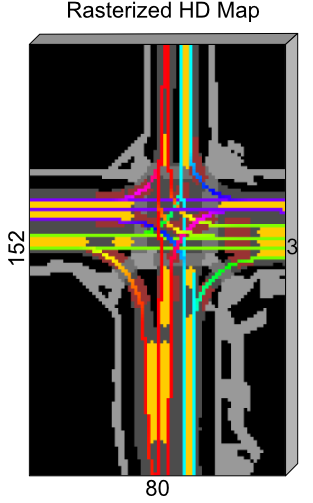
\includegraphics[width=\textwidth]{figures/caspnet-bev-repr.png}
    \caption{Rasterized BEV encoding}
    \label{fig:rasterized}
\end{subfigure}
\hfill
\begin{subfigure}[t]{0.37\textwidth}
    \centering
    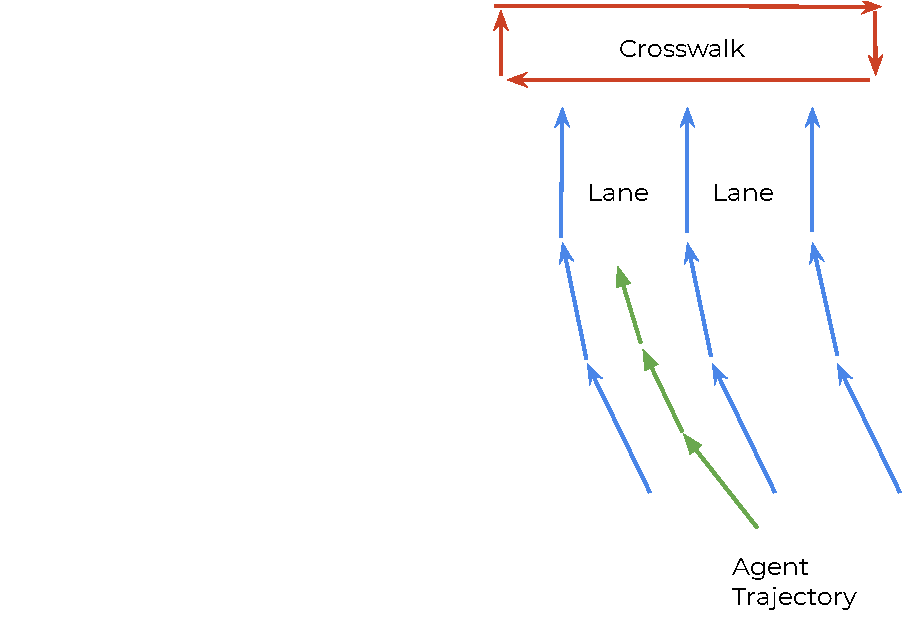
\includegraphics[width=\textwidth]{figures/vectornet-2020-vector-repr.pdf}
    \caption{Vectorized polyline preservation}
    \label{fig:vectorized}
\end{subfigure}
\caption{Scene representation paradigms in trajectory prediction: (a) rasterized approaches stack agent trajectories and HD maps into BEV images~\cite{caspnetSchäfer2022}, (b) vectorized methods preserve geometric polylines~\cite{gao2020vectornet}.}
\label{fig:scene_representations}
\end{figure}

% TODO: use \begin{description}
%   \item[]
% \end{description} instead of textbf{} to introduce the two paradigms

\begin{description}
\item[Raster grids.] Early systems stack past agent masks and HD-map layers into \( F \)-dimensional BEV (Bird's Eye View) images, leveraging convolutional backbones to capture spatial relationships while keeping runtime independent of the number of agents~\cite{cui2019multimodal,chai2019multipath}. Specifically, these approaches construct: (i) a BEV stack of past agent trajectories \( \mathbf{I}_d\in\R^{T_p\times H\times W\times F_d} \) and (ii) a static HD-map raster \( \mathbf{I}_s\in\R^{H\times W\times F_s} \).\\
The CASPNet family of motion forecasting models, consisting of the original CASPNet~\cite{caspnetSchäfer2022}, which utilizes a fully convolutional architecture, CASPNet++~\cite{caspnetppSchäfer2023}, and the CASPFormer~\cite{caspformerYadav2024}, exemplifies interesting architectural choices within this paradigm and will be discussed in greater detail in~\autoref{ssec:caspnet}.\\
However, rasterized approaches suffer from limited geometric fidelity and redundant pixel information due to grid-based discretization of scene elements' geometric and kinematic properties~\cite{lmformerYadav2025}. Additionally, respecting agent identities is infeasible as it would require separate channels per agent, introducing further redundancy; CASPNet++~\cite{caspnetppSchäfer2023} addressed this using single BEV per agent. Furthermore, rasterized approaches allow only shared coordinate systems, which is suboptimal for leveraging geometric isomorphisms~\cite{qcnetZhou2023}. % TODO: it is infeasible to respect the identities of agents as this would require a separate channel or set of channels for each agent throughout the entire architecture, which would introduce even more redundancy in terms of pixel information. However, respecting identities is crucial for true multi-agent motion forecasting, the aforementioned approach of using a single BEV per agent was used in \cite{caspnetppSchäfer2023}. Additionally, rasterized approaches allow only a shared coordinate system, which is suboptimal in terms of leverageable geometric isomorphisms.

\item[Vector representations.] Later work encodes agents and lanes as vectorized geometric primitives such as polylines, enabling graph (LaneGCN~\cite{liang2020learning}, VectorNet~\cite{VectorNet2020}) or transformer based (QCNet~\cite{qcnetZhou2023}, QCNeXt~\cite{qcnextZhou2023}, LMFormer~\cite{lmformerYadav2025}) approaches with higher geometric fidelity but runtime that grows with scene complexity. These representations are more compact, preserve higher geometric fidelity, and enable explicit modeling of complex spatio-temporal and social relationships between scene elements. Lane information uses two main representations:
\begin{itemize}
  \item \textbf{Point-based}: Each polyline \(L_p^i = [P_1^i, P_2^i, \ldots, P_K^i]\) with \(K\) control points \(P_k^i\)~\cite{VectorNet2020, zhou2022hivt}.
  \item \textbf{Segment-based}: Converts to \(L_v^i = [V_1^i, V_2^i, \ldots, V_{K-1}^i]\) where \(V_{k}^i = [P_k^i, P_{k+1}^i]\) stores lane segment vectors. This explicitly encodes road curvature~\cite{liang2020learning,zhou2022hivt,qcnetZhou2023}.
\end{itemize}
Agent trajectories use analogous representations:
\begin{itemize}
  \item \textbf{Trajectory points}: \(\mathcal{T}_{in}^a = [P_1^a, P_2^a, \ldots, P_T^a]\) with global positions \(P_t^a\).
  \item \textbf{Motion vectors}: \(M_t^a = [P_{2}^a - P_{1}^a, \ldots, P_{T}^a - P_{T-1}^a]\) derived from trajectories, representing the displacement between timesteps~\cite{lmformerYadav2025}.
\end{itemize}
Vectorized approaches employ either \emph{agent-centric} coordinate systems (all scene elements normalized to a single ego-centric frame) or \emph{query-centric} paradigms. The choice fundamentally affects computational efficiency, invariance properties, and multi-agent reasoning capabilities, with query-centric approaches offering significant advantages for streaming applications and parallel multi-agent prediction~\cite{qcnetZhou2023}. % TODO: introduce the Vector Based Representation by saying that they are more compact and preserve more geometric fidelity, they are more appropriate for the use in transformer or graph based approaches and allow to model complex spatio-temporal and social relationships between scene elements more explicitly. % TODO: elaborate more closely what agent-centric means: i.e. a single ego-centric coordinate system for all agents.
\end{description}
%% FINISHED UNTIL HERE %%
UniTraj~\cite{unitrajFeng2024} employs a vectorized and agent-centric representation, representing both agent trajectories as vertex lists and map polylines as uniformly sampled list of vertices.

% This so-called \emph{query-centric} approach will be discussed in greater detail in~\autoref{ssec:qc_paradigm}. CASPNet embodies the \emph{raster} philosophy; CASPFormer adopts a hybrid strategy—retaining a CNN backbone for perception compatibility, but switching to a vectorized transformer decoder for output precision.

\subsection{The Query-Centric Paradigm}
\label{ssec:qc_paradigm}

\paragraph{The short-comings of agent-centric approaches.}

While the agent-centric paradigm is a conceptually simple solution that aligns well with the historical focus on single-agent prediction, where the entire scene is expressed in a global frame centered on the ego vehicle, it is not well-suited for the emerging task of \emph{multi-agent} motion forecasting as it yields roto-translation and time-invariance for only the center agent~\cite{lmformerYadav2025}. \\
Furthermore, this approach becomes computationally infeasible when utilized within the framework of \emph{factorized attention}. While typical encoding strategies, such as those employed in the CASPNet family, squeeze the entire temporal dimension, and subsequently apply agent-map and agent-agent fusion on this time-invariant representation, factorized attention maintains separate spatio-temporal latent representation of all entities in the scene, allowing the model to capture more complex spatio-temporal relationships, such as the interactions between mutliple agents over the course of multiple timesteps. However, this implies cubic complexity for each fusion step:
\begin{equation}
  \begin{aligned}
    \text{Temporal:}      & \quad \mathcal{O}\!\bigl(N_{\max}T^{2}\bigr) \\
    \text{Agent\(\leftrightarrow\)Map Fusion @ $t$:}    & \quad \mathcal{O}\!\bigl(N_{\max}T K\bigr)  \\
    \text{Agent\(\leftrightarrow\)Agent Fusion @ $t$:}  & \quad \mathcal{O}\!\bigl(N_{\max}^{2}T\bigr)
  \end{aligned}
\end{equation}
where \(N_{\max}\) is the maximum number of agents, \(T = T_p + T_f\) the number of total timesteps, and \(K\) is the number of map polylines. This cubic complexity arises from the need to compute pairwise interactions between all agents and map elements at each timestep, leading to significant computational overhead in dense traffic scenarios. \\

\paragraph{Query-centric encodings}
The query-centric paradigm aims to maintain the representational capacity of factorized attention, while reducing the inference latency. The most significant downside of the agent-centric paradigm in this context is that it requires the entire scene to be re-encoded at every timestep, as the location and heading of the target agent change. This means that the model must recompute the entire scene representation for each target agent at \emph{each timestep}, leading to a significant incr6ase in computational complexity and latency, especially in scenarios with many agents and long observation windows~\cite{qcnetZhou2023}.\\

\begin{figure}[H]
  \centering
  \label{fig:qc_reference_frame}
  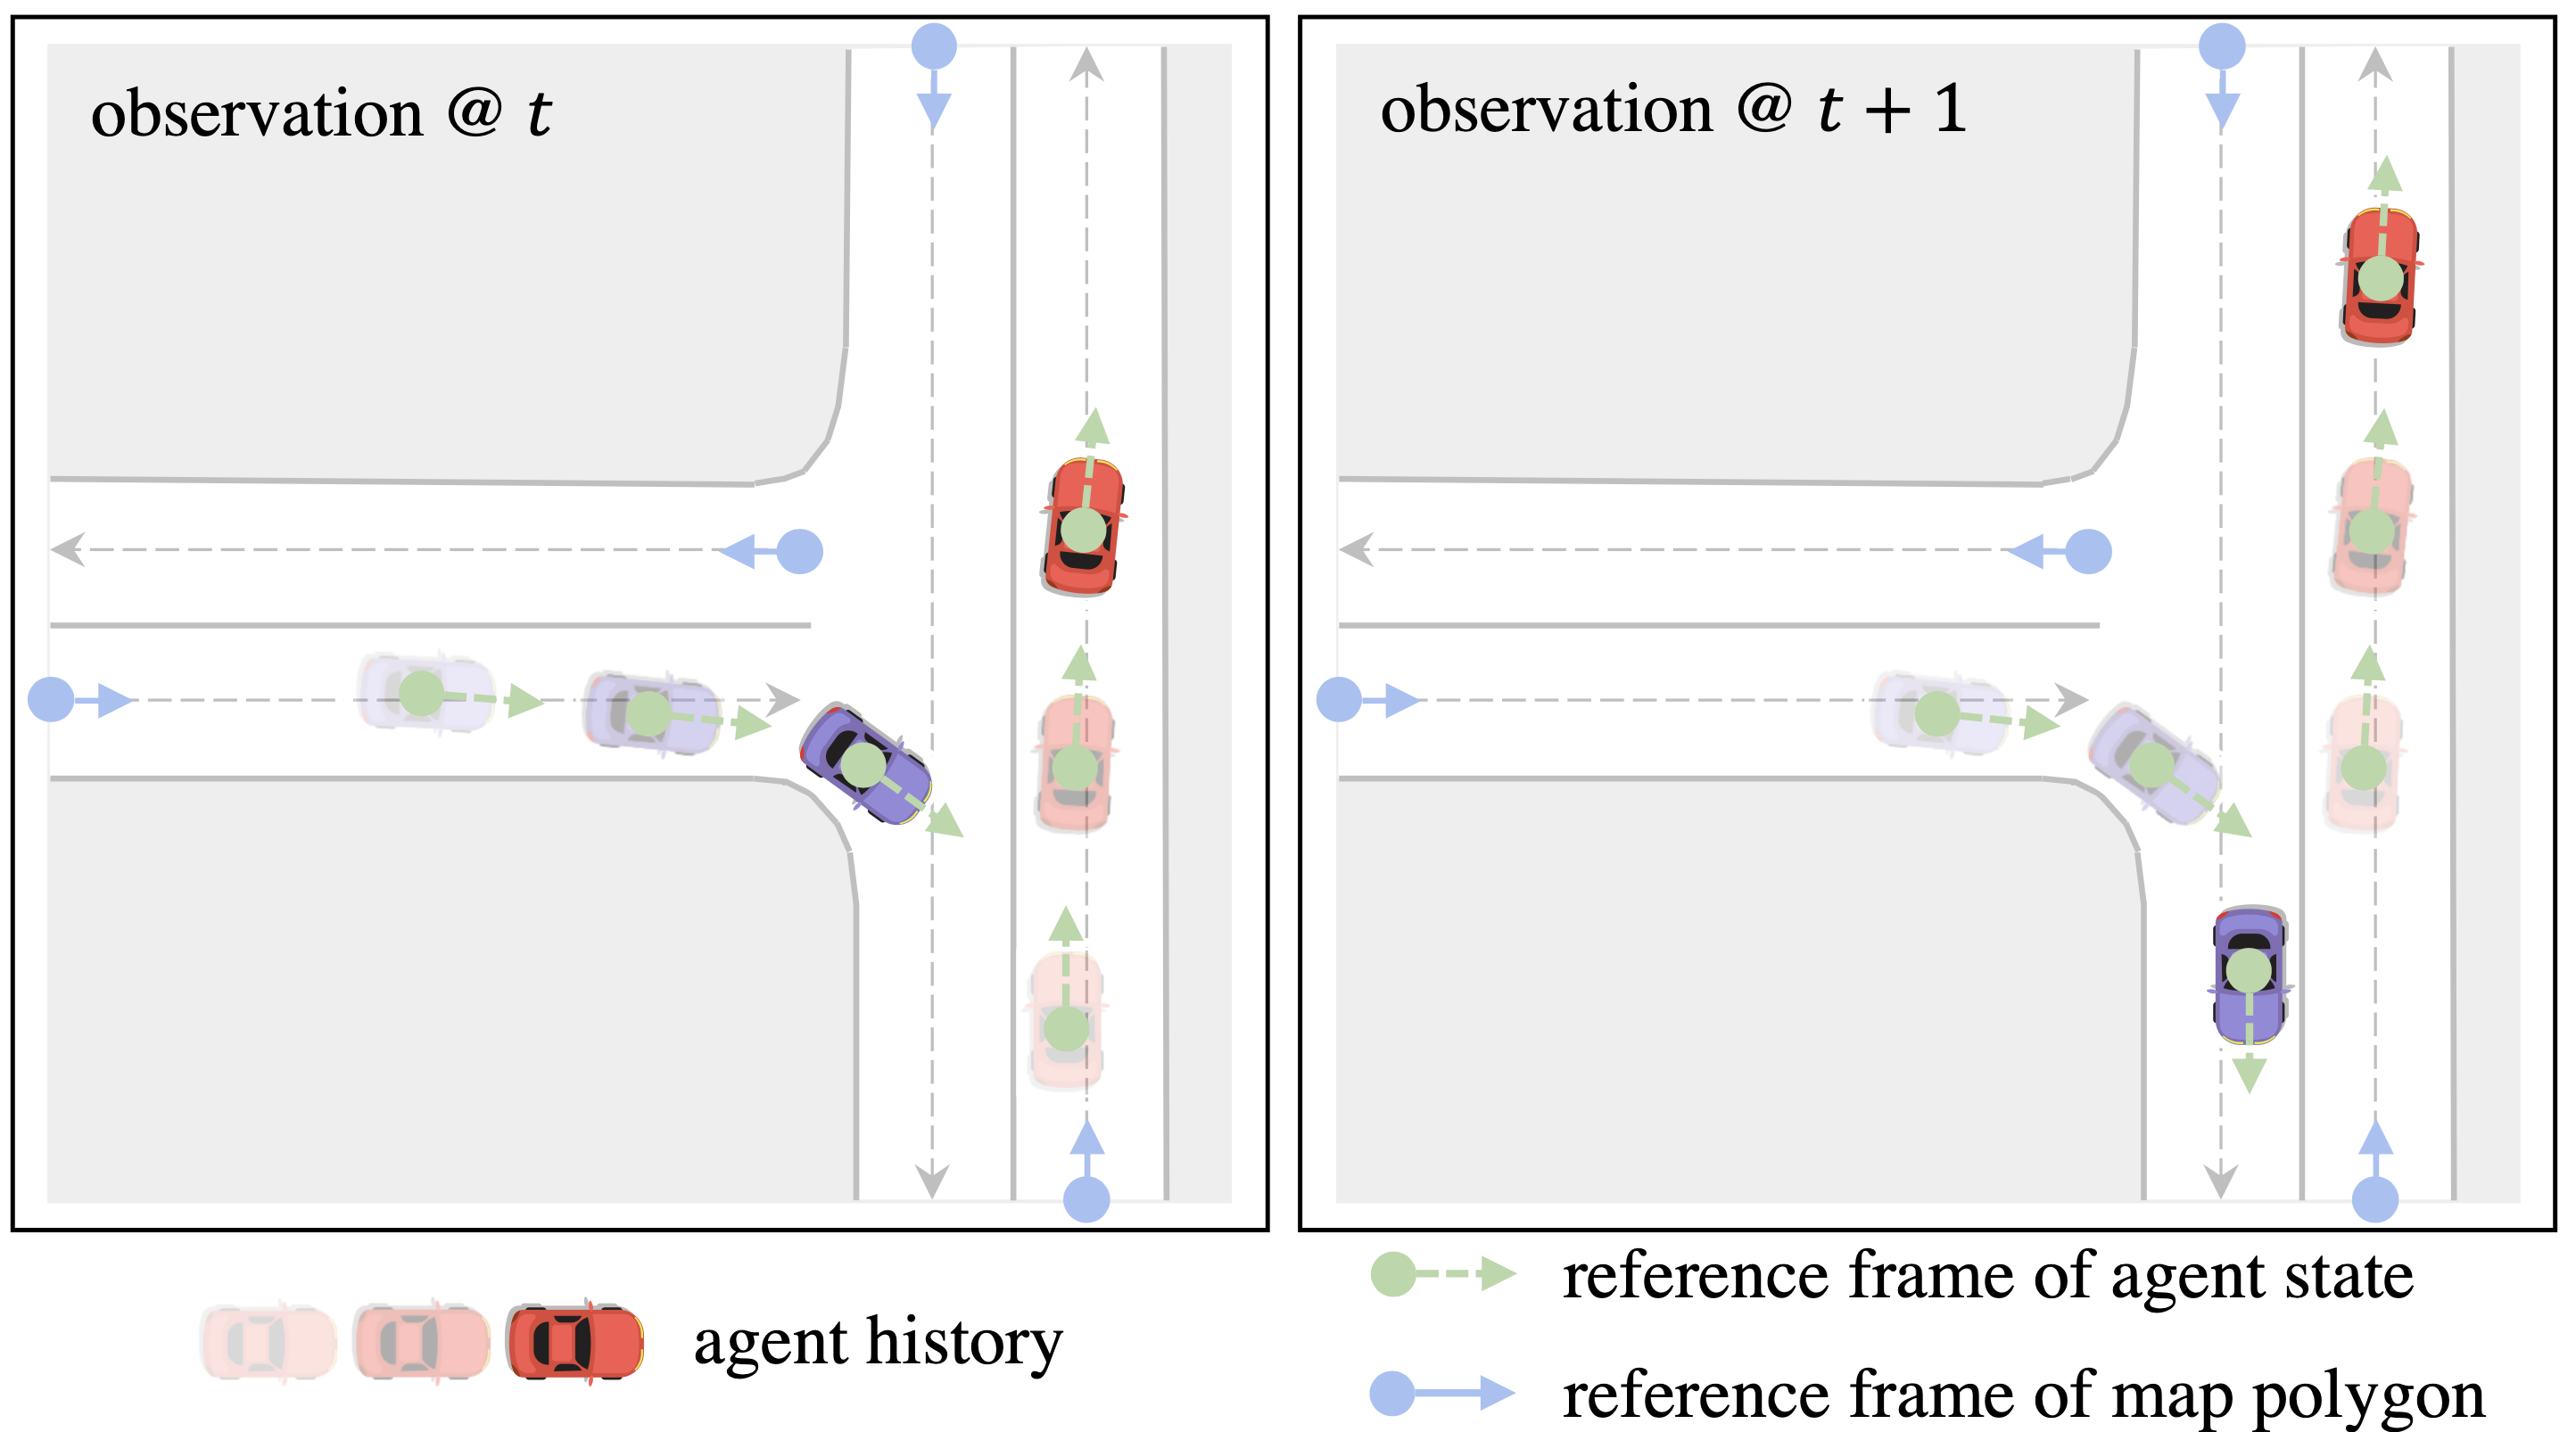
\includegraphics[width=0.5\textwidth]{figures/qc_reference_frame.png}
  \caption{\cite{qcnetZhou2023}~Query-centric encoding: each scene spatio-temporal entity lives in its own local coordinate system}
\end{figure}

Instead of expressing the scene in a single, temporally-evolving global frame, the query-centric paradigm establishes a \emph{local coordinate system} (or \emph{fiber}) for each scene element, in which all spatio-temporal and kinematic properties are expressed. This becomes especially handy, when considering that motion forecasting is inherently a \emph{streaming} task during inference: whenever a new observation arrives, the oldest observation is dropped and the newest one is added to the queue. Hence, two temporally adjacent scene representations share \(T{-}1\) overlapping timesteps, which can be cached and reused in the next step. This results in a significant reduction in computational complexity, lowering the overal runtime for each kind of fusion step by \( T \) from the cubic complexity of the agent-centric paradigm to quadratic complexity:

\begin{center}
\scriptsize
\(
\underbrace{\mathcal{O}(N_{\max}T^2)+\mathcal{O}(N_{\max}TL)+\mathcal{O}(N_{\max}^2T)}_{\text{standard factorized attention in an AC-paradigm}}
\;\longrightarrow\;
\underbrace{\mathcal{O}(N_{\max}T)+\mathcal{O}(N_{\max}L)+\mathcal{O}(N_{\max}^2)}_{\text{query-centric streaming}}
\)
\end{center}


\subsubsection*{Local frame construction}
\label{sssec:qc_local_frames}
The query-centric paradigm builds a local spacetime frame for each scene element, creating what is commonly referred to as \emph{fibres}, which can be seen as slices through the global scene manifold. The concept of fibres and more generally \emph{fiber bundles} is borrowed from differential geometry, where a fiber bundle is a structure that consists of a base space and fibers above each point in the base space, allowing for local coordinate systems to be defined independently at each point\cite{bronstein2021geometric}.

% \textbf{Geometric structure:} The scene forms a fiber bundle where the base space \(\mathcal{E}=\{e_1,\dots,e_N\}\) parameterizes scene elements, and each fiber \(F_i \cong SE(2)\) above element \(e_i\) represents the manifold of possible coordinate systems at that location. The total space is \(\mathcal{B} = \bigcup_{i=1}^N \{e_i\} \times F_i\), with projection \(\pi: \mathcal{B} \to \mathcal{E}\).

% \textbf{Symmetry preservation:} Under global transformations \(g \in SE(2)\), the entire bundle transforms as \(g \cdot \mathcal{B}\), but relative descriptors \(r_{j\to i}^{s\to t}\) between chosen frames remain invariant because they encode intrinsic geometric relationships that are independent of the global coordinate system. This invariance property is what enables the computational advantages of the query-centric approach.

With this distinction in mind, we now describe how specific local coordinate frames are constructed for different scene elements:

\begin{description}[style=nextline,leftmargin=*]
  \item[Agent states.]
        For the \(i\)-th agent at timestep \(t\), the local frame is anchored at the agent's spatial position \(\mathbf{p}_i^t = (p_{i,x}^t, p_{i,y}^t)\) with the \(x\)-axis aligned to the agent's instantaneous heading \(\theta_i^t\)~\cite{lmformerYadav2025}. The transformation from global to local coordinates is:
        \begin{equation}
            \mathbf x^{(i,t)}_{\text{local}}
            =\mathbf T_{i,t}^{-1}\,\mathbf x_{\text{global}^{(i,t)}},
            \qquad\mathbf T_{i,t} =
            \begin{bmatrix}
            \cos\theta_i^t & -\sin\theta_i^t & p_{i,x}^t \\
            \sin\theta_i^t & \cos\theta_i^t & p_{i,y}^t \\
            0 & 0 & 1
            \end{bmatrix} \in \mathrm{SE}(2).
            \label{eq:agent_frame}
        \end{equation}
        This yields \(N_{\max} \times T\) distinct fibres over the observation window, where each agent state \((\mathbf{p}_i^t, \theta_i^t, \mathbf{v}_i^t)\) defines its own reference coordinate system and \( \mathbf{x}_{\bullet}^{(i,t)} \subset \mathbf{X}_d \) represents some arbitrary spatial or kinematic vector (i.e., motion vector, velocity, ...) belonging to the \(i\)-th agent at timestep \(t\).

  \item[Map elements.]
        Lanes are represented as segment lists. Each segment's start vertex acts as the origin and the direction of the first segment defines the \(x\)-axis, leaving only the (normalized) length as an explicit feature~\cite{lmformerYadav2025}.
\end{description}

Each element's geometric attributes (velocity vectors, motion trajectories, or sampled map points) are then expressed in polar coordinates relative to their respective local frames and lifted into a higher dimensional space using encoding schemes like (learnable) Fourier features~\cite{qcnetZhou2023, li2021llearnableFourier}. These encodings can then be concatenated with the semantic attributes (e.g., agent type).

\begin{figure}[ht]
\centering
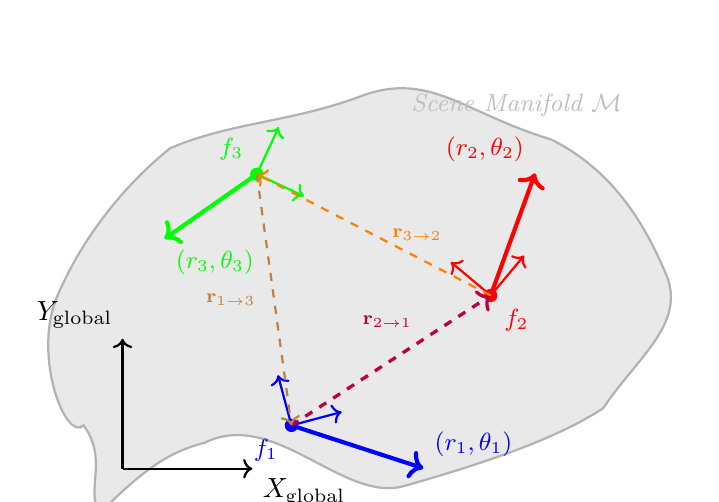
\begin{tikzpicture}[scale=1.1]

  % Complex 2D Bézier manifold passing through the origin
  % Define key points including origin (0,0)
  \coordinate (origin) at (0,0);
  \coordinate (p1) at (1.2,0.8);
  \coordinate (p2) at (3.5,0.3);
  \coordinate (p3) at (5.8,1.2);
  \coordinate (p4) at (6.5,2.8);
  \coordinate (p5) at (5.2,4.3);
  \coordinate (p6) at (3.0,4.8);
  \coordinate (p7) at (0.8,4.2);
  \coordinate (p8) at (-0.5,2.5);
  \coordinate (p9) at (-0.2,1.0);

  % Complex Bézier curve manifold with multiple control points
  \fill [gray!25, opacity=0.7]
        (origin) ..
        controls (0.5,0.5) and (0.8,0.7) ..
        (p1) ..
        controls (2.0,1.2) and (2.8,0.1) ..
        (p2) ..
        controls (4.2,0.5) and (5.2,0.8) ..
        (p3) ..
        controls (6.2,1.8) and (6.8,2.2) ..
        (p4) ..
        controls (6.2,3.5) and (5.8,4.0) ..
        (p5) ..
        controls (4.2,4.6) and (3.8,5.1) ..
        (p6) ..
        controls (2.2,4.5) and (1.5,4.5) ..
        (p7) ..
        controls (0.3,3.8) and (-0.2,3.2) ..
        (p8) ..
        controls (-0.8,1.8) and (-0.4,0.8) ..
        (p9) ..
        controls (0.1,0.6) and (-0.2,0.2) ..
        (origin) -- cycle;

  % Add manifold boundary for better visibility
  \draw [gray!60, thick]
        (origin) ..
        controls (0.5,0.5) and (0.8,0.7) ..
        (p1) ..
        controls (2.0,1.2) and (2.8,0.1) ..
        (p2) ..
        controls (4.2,0.5) and (5.2,0.8) ..
        (p3) ..
        controls (6.2,1.8) and (6.8,2.2) ..
        (p4) ..
        controls (6.2,3.5) and (5.8,4.0) ..
        (p5) ..
        controls (4.2,4.6) and (3.8,5.1) ..
        (p6) ..
        controls (2.2,4.5) and (1.5,4.5) ..
        (p7) ..
        controls (0.3,3.8) and (-0.2,3.2) ..
        (p8) ..
        controls (-0.8,1.8) and (-0.4,0.8) ..
        (p9) ..
        controls (0.1,0.6) and (-0.2,0.2) ..
        (origin);

  % Add manifold label with better positioning
  \node[gray!50, font=\small\itshape] at (4.8,4.7) {Scene Manifold $\mathcal{M}$};

  % Global Cartesian axes (origin now on manifold)
  \draw[thick,->] (0.25,0.5) -- (1.75,0.5) node[anchor=north west]{$X_{\text{global}}$};
  \draw[thick,->] (0.25,0.5) -- (0.25,2) node[anchor=south east]{$Y_{\text{global}}$};


  % Fiber positions with better spacing (adjusted to be on/near manifold)
  \coordinate (e1) at (2.2,1.0);
  \coordinate (e2) at (4.5,2.5);
  \coordinate (e3) at (1.8,3.9);

  % Fiber origins (now visible as distinct points)
  \draw[blue,fill=blue]   (e1) circle(2pt) node[below left=2pt] {\small$f_1$};
  \draw[red,fill=red]     (e2) circle(2pt) node[below right=2pt] {\small$f_2$};
  \draw[green,fill=green] (e3) circle(2pt) node[above left=2pt] {\small$f_3$};

  % Local reference frames (more prominent)
  \draw[blue,thick,->]   (e1) -- ++(15:0.6)  node[anchor=south west] {};
  \draw[blue,thick,->]   (e1) -- ++(105:0.6) node[anchor=south east] {};

  \draw[red,thick,->]    (e2) -- ++(50:0.6)  node[anchor=south west] {};
  \draw[red,thick,->]    (e2) -- ++(140:0.6) node[anchor=south east] {};

  \draw[green,thick,->]  (e3) -- ++(-25:0.6) node[anchor=north west] {};
  \draw[green,thick,->]  (e3) -- ++(65:0.6)  node[anchor=south west] {};

  % Motion vectors in local coordinates
  \draw[blue,->,line width=1.5pt]   (e1) -- ++( -18:1.6) node[anchor=south west] {\small$(r_1,\theta_1)$};
  \draw[red,->,line width=1.5pt]    (e2) -- ++(70:1.5) node[anchor=south east] {\small$(r_2,\theta_2)$};
  \draw[green,->,line width=1.5pt]  (e3) -- ++(-145:1.3) node[anchor=north west] {\small$(r_3,\theta_3)$};

  % Relative descriptors with 4D components highlighted
  \draw[purple,dashed,->,very thick] (e1) -- (e2)
    node[midway,above=8pt,align=center] {
      \scriptsize$\mathbf{r}_{2\to 1}$
    };

  % Additional relative descriptors (simpler labels for clarity)
  \draw[orange,dashed,->,thick] (e2) -- (e3)
    node[midway,right=3pt] {\scriptsize$\mathbf{r}_{3\to 2}$};
  \draw[brown,dashed,->,thick]  (e3) -- (e1)
    node[midway,left=3pt] {\scriptsize$\mathbf{r}_{1\to 3}$};

\end{tikzpicture}
\caption{Query-centric scene representation as fiber bundle: Each scene element defines a local fibre \(F_i\) with its own coordinate system \((x_i, y_i)\) embedded in the global scene manifold \(\mathcal{M}\). The colored orthogonal arrows represent specific local coordinate frames \(f_i \in F_i\) chosen from each fibre. Motion vectors \((r_i,\theta_i)\) are expressed in local polar coordinates, while relative descriptors \(\mathbf{r}_{j\to i}\) encode the 4D spatial-temporal relationships between fibres, preserving distance, bearing, orientation difference, and temporal offset.}
\label{fig:polar-frames-three}
\end{figure}


\paragraph{Relative descriptors and embeddings.}
Having established the conceptual framework of fibres and local coordinate frames, we now describe how spatial-temporal relationships between scene elements are encoded. The query-centric paradigm constructs relative positional embeddings that preserve all essential geometric information while maintaining invariance properties. For any pair of scene elements with absolute tuples \((\mathbf{p}_i^t, \theta_i^t, t)\) and \((\mathbf{p}_j^s, \theta_j^s, s)\), QCNet~\cite{qcnetZhou2023} forms a 4-dimensional descriptor:
\begin{equation}
\mathbf{r}_{j\to i}^{s\to t}=
\bigl[
    \|\mathbf{p}_j^s-\mathbf{p}_i^t\|_2,\;
    \mathrm{atan2}(p_{j,y}^s-p_{i,y}^t,\;p_{j,x}^s-p_{i,x}^t)-\theta_i^t,\;
    \theta_j^s-\theta_i^t,\;
    s-t
\bigr].
\label{eq:relative_descriptor}
\end{equation}

This descriptor fully preserves the spatial-temporal offset between elements and is designed to be invariant under global SE(2) transformations. Each component encodes a specific geometric relationship:
\begin{enumerate}[label=(\roman*)]
    \item The Euclidean distance \(\|p_j^s-p_i^t\|_2\) captures the spatial separation between elements.
    \item The angular offset \(\mathrm{atan2}(\cdot)-\theta_i^t\) represents the bearing from element \(i\) to element \(j\) in \(i\)'s local coordinate frame.
    \item The orientation difference \(\theta_j^s-\theta_i^t\) encodes the relative heading between elements.
    \item The temporal offset \(s-t\) preserves the time relationship between observations.
\end{enumerate}

Following QCNet~\cite{qcnetZhou2023}, this 4D descriptor is lifted into a high-frequency representation via Fourier features. These embeddings are then concatenated with other features to form the input sequences that will be processed by the decoder.

%%%%%%%%%%%%%%%%%%%%%%%%%%%%%%%%%%%%%%%%%%%%%%%%%%%%%%%%%%%%%%%%%%%%%%%%%%%%%%%%%%%%%%%%%%

\subsubsection*{A geometric perspective.}
\label{sssec:qc_geometric_perspective}

The query-centric paradigm exploits three fundamental symmetries that reflect the underlying physics of trajectory prediction. By placing each scene element (agent or map polygon) in its own local \(SE(2)\) coordinate frame, this approach dramatically simplifies the learning problem compared to agent-centric methods by theoretically allowing a decomposition of the global scene manifold into a composition of local fibres, each representing a standardized set of spatial and kinematic properties or relatively simple connections between different fibres.

\begin{description}[style=nextline,leftmargin=*]
\item[Permutation invariance.] % TODO: equivariance or invariance?
    Agents and map elements form an unordered set—no element should be  privileged. Query-centric approaches preserve this natural symmetry by treating all elements identically through local frames, while agent-centric methods break symmetry by choosing one agent as the global origin. Formally, for any permutation \(\sigma\) of scene elements, the encoding remains equivariant: \(f(\sigma \cdot S) = \rho(\sigma) f(S)\).

\item[SE(2) invariance.]
      Rigid translations or rotations of the entire scene must leave the encoding unchanged:
      \begin{equation}
        f_{\boldsymbol{\Psi}}\!\bigl(g\!\cdot\!S\bigr)=f_{\boldsymbol{\Psi}}(S)\qquad\forall\,g\in SE(2).
      \end{equation}
      Because every geometric attribute is expressed either in its \emph{own} local frame or as a \emph{relative} descriptor between two frames, dependencies on the global origin and its orientation never appear. \( f_{\boldsymbol{\Psi}} \) might represent solely the encoder network, or in case of the LMFormer~\cite{lmformerYadav2025} the entire architecture including the decoder.
\item[Temporal translation invariance.]
    Motion forecasting uses sliding time windows—shifting the time origin should not affect predictions. For any time shift \(\tau\in\mathbb{R}\), the representation satisfies \(f(S(t+\tau))=f(S(t))\). Query-centric methods enable efficient caching since relative temporal descriptors remain unchanged as windows slide. Agent-centric approaches violate this property because their global reference frame evolves with the target agent, requiring full re-encoding at each timestep.
\end{description}

Viewed through the lens of \emph{fiber bundles}, the global scene manifold factorises into many almost-identical \emph{fibres}—one for every agent state or lane segment—each parameterised by a small, standardised set of spatial and kinematic variables. Because all agents obey the same motion constraints and all map segments share the same geometric primitives, these fibres are essentially isomorphic.\\
Consequently, we hypothesize that the model can split its representational capacity to learning the \emph{relations between fibres}, as well as the relatively \emph{simple structures of the fibres} themselves instead of having to learn a non-decomposable global scene manifold.
The pairwise encodings of the relative descriptors \emph{connecting} the fibres inhabit an even simpler manifold, further shrinking the hypothesis space. This decomposition supplies the key inductive bias of the query-centric paradigm: by respecting permutation symmetry and \(\mathrm{SE}(2)\!\rtimes\!\mathbb{R}\) invariance, it breaks the otherwise intractable global scene manifold into a set of small, repeatable sub-manifolds connected by simple relations, yielding representations that are both more data-efficient and more interpretable than those produced by agent-centric encodings.

\paragraph{The downside of query-centric encodings.}
Query-centric (QC) models trade \emph{compute} for \emph{memory}.
Because every agent state and map segment owns a persistent token for \emph{each} timestep and because all pairwise keys/values are cached to enable streaming reuse, the scene tensor grows linearly with $N_{\max}T$ and can reach hundreds of megabytes for a single batch.
QCNet's public implementation reports\footnote{\url{https://github.com/ZikangZhou/QCNet}\label{fn:qcnet_repo}} that training a \emph{single} model on Argoverse2 requires \(\sim\!160\text{GB}\) of GPU VRAM, typically split across 8 RTX 3090\,24 GB cards.
Even on inference, caching the key-value memory for a 10 s sliding window with 128 agents can exceed 10 GB.
However, this can be dealt with by not caching the fully embedded key-value tensors, but rather the raw relative descriptors and local frames and computing the embeddings on-the-fly during training and inference as done in~\cite{lmformerYadav2025}. Furthermore, the QC paradigm can be combined with sparse attention mechanisms, such as \emph{deformable attention} as explored in \autoref{ssec:caspformer} to further reduce the memory footprint.\\
We can safely conclude that the huge memory cost in \cite{qcnetZhou2023} mostly stems from their complex architecture and the caching rather than the query centric paradigm.


% %%%%%%%%%%%%%%%%%%%%%%%%%%%%%%%%%%%%%%%%%%%%%%%%%%%%%%%%%%%%%%%%%%%%%%%%%%%%%%%%%%%%%%%%%%


% % Furthermore, the entire scene needs to be re-encoded at every timestep as the location and heading of the target agent change

% This descriptor is embedded via Fourier features and \emph{concatenated} to keys and values inside factorized attention layers. Because both elements live in local frames, \(r_{j\to i}^{s\to t}\) is itself \(SE(2)\)- and time-translation invariant, ensuring the entire representation respects the fundamental symmetries of the physical world.

% \paragraph{Scene element embedding and processing}
% For each spatial-temporal element (agent state or map point), we compute polar coordinates of its geometric attributes (velocity, motion vector, or sampled map-point positions) \emph{relative} to its local frame.
% Each polar tuple is lifted into a high-frequency representation via Fourier features~\cite{qcnetZhou2023}, concatenated with semantic tags (e.g., agent type), and passed through an MLP to yield an embedding.
% Since each element's embedding is tied only to its own frame, it can be reused across windows, unlike agent-centric methods that must re-encode everything per agent per step.

% Map polygons undergo self-attention where query from polygon \(i\) attends to neighbors \(\{\mathbf{m}_j\}_{j\in\mathcal N_i}\), with key/value formed by \([\mathbf{m}_j;\mathbf{r}_{j\to i}]\).
% Since all components are query-centric, the output encodings are roto-translation invariant and can be shared across agents or pre-computed offline.

% For agent encoding, factorized attention enables the \(i\)-th agent at time \(t\) to attend: (1)~temporally to past \(\tau\) steps \(\{[\mathbf{a}_i^s;\mathbf{r}_{i\to i}^{s\to t}]\}_{s=t-\tau}^{t-1}\), (2)~spatially to map elements \(\{[\mathbf{m}'_j;\mathbf{r}_{j\to i}]\}_{j\in\mathcal N_i}\), and (3)~socially to neighboring agents \(\{[\mathbf{a}_j^t;\mathbf{r}_{j\to i}^{t\to t}]\}_{j\in\mathcal N_i}\).
% This enables the crucial complexity reduction:



% \paragraph{Agent-centric vs.\ query-centric comparison.}

% \begin{description}[style=nextline,leftmargin=*]
%   \item[Computational efficiency and reuse.]
%         Agent-centric: None—recompute full BEV/agent tokens each step (\(O(A T^2)\)); query-centric: Cache and reuse—when the window slides, the \(T-1\) overlapping steps' embeddings are identical and can be reused, reducing cost to \(O(A T)\) and enabling \(<\!10\)ms latency in dense scenes. However, this efficiency comes at a memory cost, as QCNet training consumes approximately 160GB GPU memory~\cite{qcnetZhou2023}.
%         Encodings are independent of prediction target and can be shared across agents and time steps.
%   \item[Symmetry preservation and multi-agent reasoning.]
%         Agent-centric breaks permutation symmetry by privileging one agent; query-centric treats all elements equally, preserving the natural symmetry among multiple agents and enabling true joint prediction rather than marginal approaches.
%         Parallel decoding: Usually one-agent-at-a-time for agent-centric; multi-agent parallel with the same invariant scene tensor shared by all target agents for query-centric.
%   \item[Streaming and invariance properties.]
%         Query-centric caches invariant tensors across sliding windows and supports parallel prediction for all agents using the same scene encoding; agent-centric re-normalizes each step and requires separate encodings per agent.
%         Latent scene representations are \(SE(2) \rtimes \R\) invariant through the relative descriptors.
%   \item[Memory vs.\ computation trade-off.]
%         QCNet's tensors are shared by all targets but grow linearly with scene size; large-scene training can hit GPU limits.
%         Agent-centric stores fewer per-element relations but recomputes them repeatedly.
%   \item[Inductive bias and learning efficiency.]
%         Efficient reuse: Encodings are independent of prediction target and can be shared across agents and time steps.
%         Local fibers (all isomorphic to \(SE(2)\)) mean the network only learns relations \emph{between} fibers; the sub-manifold to model is smaller, requiring less representational capacity~\cite{bronstein2017geometric}.
%         This dramatically shrinks the global manifold of possible scene encodings compared to agent-centric approaches.
%         Joint prediction capability: Unlike marginal prediction approaches, query-centric models can effectively capture future social interactions among agents.
% \end{description}

% \paragraph{Take-away.}
% By framing scene elements as fibers over \(SE(2)\) and encoding only \emph{relative} pose/time, query-centric representations furnish strong geometric inductive biases, enable massive computation reuse, and support truly parallel multi-agent decoding. These qualities underlie QCNet~\cite{qcnetZhou2023}, LMFormer~\cite{lmformerYadav2025}, and related trajectory prediction models that leverage this paradigm.


%%%%%%%%%%%%%%%%%%%%%%%%%%%%%%%%%%%%%%%%%%%%%%%%%%%%%%%%%%%%%%%%%%%%%%%%%%%%%%%%%%%%%%%%%%%

%<unstructured-collection-of-information-to-include>
% <include:1>\cite{lmformerYadav2025} into Local frame construction
% TODO: define how each local coodinate frame is defined:
% agents: motion vector's start position as its origin, x axis is instantaneous direction of travel
% map polylines: very lane segment is characterized by its start and end positions in global coordinates. The query-centric coordinate frame for a lane segment is set as follows: we designate the segment's start position as its origin and align the segment's vector direction with its x-axis. As a result, the only feature preserved in this query-centric coordinate frame is the segment's length, which we use as its sole feature in the query-centric embedding generation.
% BOTH of these conventions stem from \cite{lmformerYadav2025}
% </include:1>
% <include:2> in Agent-centric vs. query-centric comparison
% Parallel decoding Usually one-agent-at-a-time for agent centric. Multi-agent parallel: same invariant scene tensor is shared by all target agents for query-centric.
% Latent scene representations are \( SE(2) \rtimes \R \) invariant (What about the impact of the relative descriptors?).
% Memory reuse Agent-Centric:% None → recompute full BEV / agent tokens each step. QC: Cache & reuse: when the window slides, the T-1 overlapping steps' embeddings are identical and can be reused. This makes the implementation in \cite{qcnetZhou2023} efficient in terms of its time complexity but it comes at a hughe memory cost, eg The training process consumes ~160G GPU memory.
% </nclude:2>
% 	1.	Local spacetime frame construction
% <include:1>
% •	Each agent state (p^t_i,\theta^t_i,v^t_i) and each map polygon has its own 3-DOF coordinate frame: origin = current position, x-axis = heading, time axis = current step.
% </include:1>
% 	4.	QC allows for Factorised attention with query-centric keys/values. What are the advantages.
	% •	Three axes: Temporal, Agent-Map, Social (Agent-Agent).
	% •	Because queries/keys include relative embeddings, all outputs remain invariant → can be cached. (Page 3-4) _Query-Centric_Trajectory_Prediction_CVPR_2023_paper-2.pdf](file-service://file-MYr4iwPvX6YAGHzdpzXMma)

% \subsubsection*{The Agent-Centric Paradigm: Progress and Limitations}

% \textbf{Agent-centric normalization:} To attain translation and rotation invariance for a target agent, this scheme re-centers and rotates the entire scene so that the reference agent sits at the origin facing the positive $x$-axis. Although this stabilizes coordinate scales and simplifies learning for that agent, privileging one agent breaks permutation symmetry among multiple agents and demands redundant re-normalization and re-encoding each time the prediction target or time window changes, resulting in substantial computational overhead in streaming and multi-agent settings.

% To address the shortcomings of global encoding, the agent-centric paradigm normalizes all scene elements relative to a designated reference agent—typically the prediction target. By placing the reference agent at the origin and aligning its heading with the positive $x$-axis (see Equation~\ref{eq:agent_centric_transform}), agent-centric encoding offers:
% \begin{itemize}
%     \item \textbf{Translation Invariance:} Scene layouts become independent of their absolute location.
%     \item \textbf{Rotation Invariance:} Aligning the agent's heading simplifies learning of common maneuvers.
%     \item \textbf{Consistent Scale:} Bounded coordinate values improve training stability. In query centric encodigngs the range of possible values is more strongly bounded.
%     \item \textbf{Ego-View:} Mirrors the vehicle's own perspective (all vehicles live in fibers that are quite similar to each other), hence the same features are to be expected for all agents independent of their position. This dramatically shrinks the global manifold of possible scene encodings, making it easier for the model to learn efficient representations through *strong inductive biases* % TODO: how is this redundant from the first two points (translation and rotation invariance)
% \end{itemize} % TODO: mention the symmetries only briefly here and add a new \begin{describe} subsequently $[isomorphisms] to discuss the symmetries in more detail.
% <include:3> shortcomings of agent-centric encoding
% Despite these advantages, agent-centric encoding introduces new challenges:
% \begin{itemize}
%     \item \textbf{Computational Redundancy:} Every change in the prediction target or sliding time window requires re-normalizing and re-encoding the entire scene.
%     \item \textbf{Broken Permutation Symmetry:} Privileging one agent as origin disrupts the natural symmetry among multiple agents, hindering true joint prediction.
%     \item \textbf{Temporal Inconsistency:} Streaming applications incur unnecessary reprocessing of static map elements as the reference frame shifts.
%     \item \textbf{Multi-Agent Inefficiency:} Parallel prediction for multiple agents multiplies encoding costs linearly with the number of agents.
% \end{itemize}
% </include:3> shortcomings of agent-centric encoding

% <include:2> in Agent-centric vs. query-centric comparison
% \begin{itemize}
%     \item \textbf{Efficient reuse:} Encodings are independent of prediction target and can be shared across agents and time steps.
%     \item \textbf{Permutation symmetry:} No agent is privileged; all elements are represented equally.
%     \item \textbf{Multi-agent and streaming:} The same scene encoding can be used for parallel prediction of all agents and for streaming updates.
%     \item \textbf{Joint prediction capability:} Unlike marginal prediction approaches, query-centric models can effectively capture future social interactions among agents.
% \end{itemize}
% </include:2>

% %$[isomorphisms]
% <include:4> in Symmetry group actions -> rename A Geometric Perspective on Scene Representations
% here we need to cite~\cite{bronstein2021geometric}
% \begin{itemize}
%     \item \textbf{Permutation symmetry:} The set of agents and map elements is unordered. The model should be equivariant to permutations of the input.
%     \item \textbf{$\SE(2)$ symmetry:} The laws of physics are invariant under translation and rotation. The model should be equivariant to global $\SE(2)$ transformations.
%     \item \textbf{Temporal symmetry:} The encoding should be invariant to shifts in the time origin (for streaming).
% \end{itemize}
% we want to use this perspective of fiber bundels to explain the symmetries - i.e. the sub manifold of all the agents (where spatial and kinematic properties are represented) are quite similar - hence smaller, hence easier to learn. This is the key inductive bias of the query-centric paradigm, which is not present in the agent-centric paradigm. Same goes for the static map elements.
% And the part of the part of the latent scene representation that encodes the relative spatio-temporal relationships between scene elements is in total much smaller and hence also doesn't require as much representative capacity in the model.
% </include:4> Symmetry group actions -> rename A Geometric Perspective on Scene Representations



% The use of \emph{query-centric} scene encodings~\cite{qcnetZhou2023} represents a paradigm shift in trajectory prediction for autonomous driving, fundamentally altering how the spatio-temporal attributes of both static (agents) and dynamic (map polylines) scene elements are represented. <include:introduction>The query-centric paradigm is grounded in the concept of relative spacetime manifolds, drawing inspiration from Einstein's theory of relativity, where the coordinates of scene elements are not expressed in a \emph{global} or \emph{agent-centric} coordinate system</include:introduction>, but rather in \emph{local} frames defined by each element itself. This approach introduces various symmetries, that can be explored through the lens of differential geometry and geometric deep learning~\cite{bronstein2021geometric}, allowing for the design of models leveraging these inductive biases, resulting in more robust and efficient model architectures. This chapter outlines the limitations of traditional agent-centric encoding schemes and provides a comprehensive overview of the query-centric paradigm, including its mathematical foundations, encoding strategies, and architectural innovations.


% QCNet generalizes vector-based encoders by abandoning a single ego-centric grid in favor of local `fibers' for every map polygon or agent-state, yielding strict roto-translation and temporal invariance while enabling streaming-time reuse~\cite{qcnetZhou2023}. Each map polygon and each agent \emph{state} owns a local spacetime frame \((p,\theta,t)\) (Fig.~\ref{fig:polar-frames-three}). All geometry is expressed in these frames; relative descriptors \([\lvert\lvert p_j-p_i\rvert\rvert_2,\;\Delta\theta_{\text{dir}},\;\Delta\theta_{\text{ori}},\;\Delta t]\) are Fourier-MLP embedded and concatenated to keys/values in factorised attention. Consequently the scene tensor is \textbf{roto-translation \& time invariant}, can be \textbf{cached across sliding windows}, and is \textbf{shared by every target agent}, lowering online complexity from \(O(AT^2)\) to \(O(AT)\)~\cite{qcnetZhou2023}.



% In summary, the query-centric paradigm provides a principled, symmetry-respecting, and efficient foundation for trajectory forecasting. The combination of local polar encodings and relative descriptors yields a flexible and lossless representation, underpinning the success of recent state-of-the-art models. This approach has fundamentally changed how the community thinks about scene representation for autonomous driving, moving from agent-centric to truly democratic, multi-agent reasoning systems.
%</unstructured-collection-of-information-to-include>
%
% 3. Data Corpus and Preprocessing Methodology
\section{The Need for Unification}
\label{ch:data_methodology}

This section presents an overview of the need for a unified framework for trajectory prediction in autonomous driving, addressing the challenges of dataset heterogeneity and the complexities of motion forecasting tasks. The discussion highlights the importance of standardizing data formats, feature characteristics, and preprocessing pipelines to enable effective model training and evaluation across diverse datasets.

\subsection{Unification of Motion Forecasting Datasets}
\label{sec:data_datasets}

The \texttt{UniTraj} framework addresses the fundamental challenge of standardizing multiple motion-forecasting datasets that exhibit substantial heterogeneities in both \emph{data formats} and \emph{feature characteristics}.
The former encompasses differences in data structure and organization, while the latter stems from variations in
spatio-temporal resolution, coverage range, and semantic annotation schemes.

To overcome format discrepancies, \texttt{UniTraj} leverages \texttt{ScenarioNet}~\cite{scenarionetLi2023} for conversion into a common
format, thereby eliminating the need for multiple preprocessing implementations. However, feature characteristics require additional harmonization. Temporal coverage varies substantially
across datasets, with historical trajectories ranging from 1 second in \texttt{WOMD}\cite{wmodSun2020} to 5 seconds in \texttt{Argoverse 2}\cite{av2Wilson2023},
and future prediction horizons extending from 6 to 8 seconds. Map resolutions and semantic annotations differ
significantly, with all datasets providing \emph{scene-centric} HD maps at varying resolutions.
Agent features also exhibit substantial variations: \texttt{nuScenes} provides only velocity and heading, while
\texttt{WOMD} includes comprehensive 3D bounding box annotations. Notably, \texttt{Argoverse 2} provides bounding
box and rich semantic annotations, but these are lost during \texttt{ScenarioNet} format conversion.
The normalization of the feature spaces is performed through a multi-stage processing, and its results are outlined in~\autoref{app:framework}.


% The UniTraj framework integrates three major autonomous driving datasets: Argoverse2 (AV2)~\cite{av2Wilson2023}, NuScenes~\cite{caesar2020nuscenes}, and Waymo Open Dataset~\cite{wmodSun2020}. Each dataset contributes unique characteristics:

% \begin{itemize}
%     \item \textbf{Argoverse2:} High-resolution HD maps with detailed lane topology, focusing on highway and urban scenarios
%     \item \textbf{NuScenes:} Multi-modal sensor data with 360° coverage, diverse weather and lighting conditions
%     \item \textbf{Waymo:} Large-scale dataset with consistent labeling and comprehensive scene coverage
% \end{itemize}

% The amalgamation strategy standardizes coordinate systems, temporal sampling rates, and feature representations across datasets~\cite{VectorNet2020, Shi2022MTR}. This unified approach enables cross-dataset training and evaluation while preserving dataset-specific characteristics through metadata annotations.

% The fusion methodology addresses inherent dataset heterogeneities through a nine-phase preprocessing pipeline (detailed in Appendix~\ref{app:notation}) that transforms raw data into consistent \texttt{DatasetItem} representations. This approach follows established practices in trajectory prediction literature~\cite{zhou2022hivt, qcnetZhou2023, Shi2023MTRplusplus}.

% \subsection{Remaining ML Infrastructure}
% This subsection outlines the need for further essential components required to develop motion forecasting models, and why it would be beneficial to unify them in a single framework such that the research communicty can focus on the model architecture and training, rather than the implementation details of the infrastructure.
% This includes logging and experiment tracking, distributed training, configuration management, evaluation metrics, visualization tools




\subsection{Limitations of UniTraj}
\label{sec:data_challenges}

Implementation of the unified framework revealed significant challenges affecting data quality and model generalizability, aligning with known issues in autonomous driving dataset integration.

When creating unified dataset, given multiple source datasets, they did not respect the original train, val, and test splits which is a common practice in machine learning

None of the most important sym

\subsection{Data Integration and Representational Limitations}
\label{ssec:data_limitations}

Critical limitations emerged during dataset integration, reflecting broader challenges in autonomous driving data standardization~\cite{hu2023planning}. Dataset heterogeneity manifests through inconsistent feature availability: Agent type availability varies inconsistently—while Waymo provides comprehensive pedestrian and cyclist annotations, Argoverse2 focuses primarily on vehicle trajectories, creating domain-specific biases~\cite{unitrajFeng2024}.\\
Temporal and spatial standardization introduces information loss, highlighting trade-offs between unification and data fidelity. Varying sampling rates (10Hz vs 20Hz) require interpolation that potentially loses behavioral nuances. Feature quantization for computational efficiency reduces predictive accuracy, while fixed scene radii exclude relevant distant objects affecting long-range interactions.

\subsection{Framework Implementation Issues and Mitigation Strategies}
\label{ssec:framework_issues}

The original UniTraj implementation suffered from critical software quality deficiencies that significantly impacted model performance and generalization across domains~\cite{metadriveLi2022}. The most significant limitation was the absence of PyTorch Lightning integration, forcing manual implementation of training infrastructure that modern ML frameworks provide standardized~\cite{falcon2019pytorch}. Additional problems included poor code organization with tight coupling between components, lack of modular design patterns, and insufficient testing frameworks, making the system difficult to maintain, extend, or debug effectively.
The training infrastructure lacked essential deep learning capabilities: automatic mixed precision training, gradient accumulation, learning rate scheduling, and distributed computing support. Manual implementation of these features resulted in suboptimal performance, excessive memory usage, and limited scalability. The framework also lacked integrated experiment tracking with tools like Weights \& Biases or TensorBoard, hampering reproducibility and systematic model development workflows.
Mitigation strategies follow modern ML engineering best practices, with PyTorch Lightning migration as the primary solution. This architectural change provides structured training loops, automatic optimization, distributed computing support, and seamless experiment tracking integration~\cite{falcon2019pytorch}. Additional improvements include codebase refactoring into modular components, comprehensive unit and integration testing implementation, continuous integration adoption, and enhanced logging capabilities through Lightning's callback system for better visibility into training dynamics across datasets~\cite{unitrajFeng2024, scenarionetLi2023}.


\subsubsection{Revision of the UniTraj Framework}
This section details the major modifications we applied to the original UniTraj framework to achieve a more modular, type-safe, and production-ready codebase.

\paragraph{Data handling and preprocessing refinements.}
\begin{itemize}[leftmargin=*]
  \item \textbf{Strongly typed interfaces:} Introduced \href{https://github.com/JanDuchscherer104/UniTraj/blob/main/unitraj/datasets/types.py}{\texttt{types.py}} to declare all input and output tensors via \texttt{TypedDict} and dataclasses, replacing untyped \texttt{dict} passes and surfacing shape mismatches at static analysis time. Defines \texttt{RawScenarioDict}, \texttt{ProcessedDataDict} and other interfaces.
  \item \textbf{Decoupled parsing pipeline:} Split the monolithic script into three stages—\href{https://github.com/JanDuchscherer104/UniTraj/blob/main/unitraj/datasets/base_dataparser.py}{\texttt{base\_dataparser.py}} (handles raw file ingestion and basic conversions), \href{https://github.com/JanDuchscherer104/UniTraj/blob/main/unitraj/datasets/dataparser.py}{\texttt{dataparser.py}} (implements the nine-phase QC preprocessing pipeline), and \href{https://github.com/JanDuchscherer104/UniTraj/blob/main/unitraj/datasets/base_dataset.py}{\texttt{base\_dataset.py}} (wraps processed data into a PyTorch \texttt{Dataset} class), enabling modular parser swaps without code changes.
  \item \textbf{PyTorch Lightning integration:} Built a \href{https://github.com/JanDuchscherer104/UniTraj/blob/main/unitraj/lightning/lit_datamodule.py}{\texttt{lit\_datamodule.py}} (defines \texttt{LightningDataModule}) and \href{https://github.com/JanDuchscherer104/UniTraj/blob/main/unitraj/lightning/lit_trainer_factory.py}{\texttt{lit\_trainer\_factory.py}} (instantiates \texttt{pl.Trainer} from config) to configure \texttt{pl.Trainer} via YAML, unlocking multi-GPU, mixed-precision, and gradient accumulation with <30LoC of overhead and removing ~300LoC of boilerplate.
  \item \textbf{Full Weights \& Biases (WandB) support:} Added \href{https://github.com/JanDuchscherer104/UniTraj/blob/main/unitraj/configs/wandb_config.py}{\texttt{wandb\_config.py}} (configures WandB logger and callbacks) and Lightning callbacks to log hyperparameters, metrics, and checkpoint artefacts directly to WandB, replacing ad-hoc CSV dumps and enabling real-time dashboards.
\end{itemize}

\paragraph{Architecture Overview}
The revised UniTraj framework follows a hierarchical configuration-driven architecture that enables modular component instantiation and type-safe data flow. Figure~\ref{fig:unitraj_data_architecture} illustrates the core data handling components and their relationships within the framework.

\begin{figure}[htbp]
    \centering
    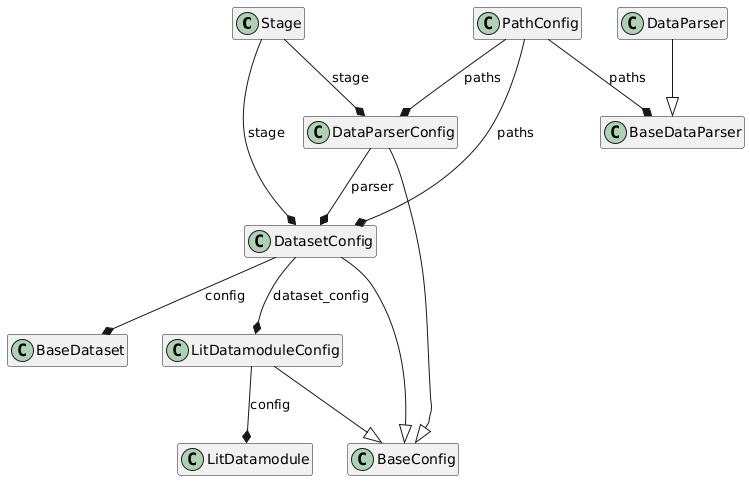
\includegraphics[width=0.9\textwidth]{figures/classes_DataHandling.png}
    \caption{UniTraj data handling architecture showing the relationships between configuration classes, data parsers, datasets, and Lightning modules. The diagram illustrates the Config-as-Factory pattern implementation and the modular data processing pipeline.}
    \label{fig:unitraj_data_architecture}
\end{figure}

The architecture comprises four primary layers:

\begin{itemize}[leftmargin=*]
    \item \textbf{Configuration Layer:} The \texttt{BaseConfig} class serves as the foundation for all configuration objects, implementing the Config-as-Factory pattern through the \texttt{setup\_target()} method. The \texttt{PathConfig} centralizes all filesystem paths and is automatically propagated to child configurations during instantiation. The \texttt{Stage} enum defines dataset splits (train/validation/test) and ensures consistent stage handling across the pipeline.
    
    \item \textbf{Data Processing Layer:} The \texttt{BaseDataParser} provides the interface for raw data ingestion, while \texttt{DataParser} implements the nine-phase preprocessing pipeline that transforms ScenarioNet format into normalized feature representations. The \texttt{DataParserConfig} controls preprocessing behavior including multiprocessing settings, cache management, and debug mode configuration.
    
    \item \textbf{Dataset Layer:} The \texttt{BaseDataset} wraps processed data into PyTorch-compatible format, implementing efficient data loading with optional H5PY file handles for large-scale datasets. The \texttt{DatasetConfig} manages dataset instantiation parameters and integrates the parser configuration for end-to-end data pipeline control.
    
    \item \textbf{Lightning Integration Layer:} The \texttt{LitDatamodule} provides PyTorch Lightning-compatible data loading with automatic train/validation/test split handling, configurable batch sizes, and multiprocessing support. The \texttt{LitDatamoduleConfig} enables declarative dataloader configuration from YAML files while maintaining type safety through Pydantic validation.
\end{itemize}

The composition relationships shown in the diagram reflect the framework's dependency injection approach: configurations contain references to their dependencies rather than hard-coded instantiations, enabling flexible component swapping and comprehensive testing. For instance, the \texttt{DatasetConfig} contains both a \texttt{DataParserConfig} and stage information, allowing different parsing strategies per dataset split without code duplication.

\paragraph{Configuration and path management.}
\begin{itemize}[leftmargin=*]
  \item \textbf{Config-as-Factory pattern:} Implemented \href{https://github.com/JanDuchscherer104/UniTraj/blob/main/unitraj/utils/base_config.py}{\texttt{base\_config.py}} (defines \texttt{BaseConfig} and \texttt{setup\_target()}) methods, allowing declarative instantiation of datasets, trainers, and models from YAML/JSON without touching code.
  \item \textbf{Centralized PathConfig:} Consolidated all filesystem paths (data root, logs, checkpoints) in \href{https://github.com/JanDuchscherer104/UniTraj/blob/main/unitraj/configs/path_config.py}{\texttt{path\_config.py}} (centralizes filesystem paths) and ensured automatic directory creation, eliminating scattered \texttt{os.makedirs()} calls.
  \item \textbf{Experiment reproducibility:} Integrated hierarchical overrides and \href{https://github.com/JanDuchscherer104/UniTraj/blob/main/unitraj/utils/base_config.py}{\texttt{base\_config.py}} (provides \texttt{inspect()} for config trees) to print the full resolved config tree at startup, improving traceability of parameter sweeps.
\end{itemize}

\paragraph{General refactoring and model zoo expansion.}
\begin{itemize}[leftmargin=*]
  \item \textbf{Modular model registry:} Refactored the \texttt{models/} folder into sub-packages (e.g., \texttt{autobot}, \texttt{mtr}, \texttt{wayformer}), each with its own \href{https://github.com/JanDuchscherer104/UniTraj/blob/main/unitraj/models/base_model/base_model.py}{\texttt{base\_model.py}} (defines \texttt{BaseModel} and \texttt{BaseModelConfig}), standardizing the interface for adding new architectures.
  \item \textbf{Utility consolidation:} Moved logging, console output, and visualization routines into \href{https://github.com/JanDuchscherer104/UniTraj/blob/main/unitraj/utils/console.py}{\texttt{console.py}} (provides structured \texttt{Console} API) modules, replacing ad-hoc print statements with a structured \texttt{Console} API.
  \item \textbf{Typed function signatures:} Audited all \texttt{.py} files to add precise type annotations for inputs and outputs (e.g., \texttt{batch: list[DatasetItem] -> BatchDict}), enabling \texttt{mypy} enforcement and catching runtime errors early.
\end{itemize}

\newpage
\section{Data Methodology within UniTraj}
\label{sec:data_methodology}

This section presents the data processing methodology within the UniTraj framework~\cite{unitrajFeng2024}, covering the transformation from heterogeneous autonomous driving datasets to standardized tensor representations suitable for trajectory prediction models. UniTraj serves as a unified interface that harmonizes datasets from WOMD~\cite{WOMD2021}, Argoverse2~\cite{av2Wilson2023}, and nuScenes~\cite{caesar2020nuscenes} through the ScenarioNet format~\cite{scenarionetLi2023}.

\subsection{UniTraj's Data Processing Pipeline}
\label{ssec:data_pipeline}

The UniTraj preprocessing pipeline transforms raw, heterogeneous data into standardized, model-ready tensors through a multi-phase process. Each phase is implemented as a distinct method within the \texttt{DataParser} class, ensuring modularity and clarity. The following provides a brief qualitative overview of the pipeline; for detailed implementations and more comprehensive descriptions, see ~\autoref{app:framework}.

\begin{description}
    \item[Phase 1: Temporal Window Extraction] Extracts fixed-length time windows from raw trajectories and applies frequency masking for uniform temporal sampling (\autoref{alg:phase1_temporal}).
    \item[Phase 2: Map Feature Processing] Converts raw map data (lanes, boundaries) into standardized polylines with uniform point density and semantic encodings (\autoref{alg:phase2_map}).
    \item[Phase 3: Agent Selection] Filters for relevant agents based on motion and observation quality to identify suitable prediction candidates (\autoref{alg:phase3_filtering}).
    \item[Phase 4: Coordinate Transformation] Transforms the entire scene into an agent-centric coordinate frame for each candidate, ensuring translation and rotation invariance (\autoref{alg:phase4_transform}).
    \item[Phase 5: Feature Assembly] Constructs comprehensive feature vectors for each agent, concatenating spatial, kinematic, and semantic attributes (\autoref{alg:phase5_features}).
    \item[Phase 6: Proximity Filtering \& Padding] Selects the \(N_{\max}\) closest agents and pads the agent tensor to a fixed size for batching (\autoref{alg:phase6_proximity}).
    \item[Phase 7: Map Tensorization] Segments, resamples, and selects the \(K_{\max}\) closest map polylines, creating a fixed-size map tensor (\autoref{alg:phase7_map_features}).
    \item[Phase 8: Future Processing] Processes and transforms the ground truth future trajectories for the center agent (\autoref{alg:phase8_future}).
    \item[Phase 9: DatasetItem Assembly] Assembles all processed tensors and masks into a final \texttt{DatasetItem}, the fundamental unit of the dataset (\autoref{alg:phase9_assembly}).
\end{description}

\paragraph{The \texttt{BaseDataParser} Class.}
The \texttt{BaseDataParser} serves as the central orchestrator of the data processing pipeline. It coordinates the parallel processing of scenario chunks, manages HDF5 file storage of the resulting dataset, and assembles the metadata that is collected throughout the pipeline.\\

\subsection{The UniTraj DatasetItem and Batching}
\label{ssec:unitraj_dataset}

The output of the processing pipeline is a collection of \texttt{DatasetItem} instances, each encapsulating a complete prediction scenario in a standardized format.

\paragraph{The \texttt{DatasetItem} Structure.}
A \texttt{DatasetItem} is a strongly typed object that holds all the \texttt{numpy} arrays corresponding to a single, agent-centric view of a scene. This includes the historical agent states, the map geometry, ground truth future trajectories, and associated validity masks. The \texttt{DatasetItem} contains all necessary data for training, evaluation, analysis and visualization, and hence contains many redundant features.

\paragraph{Batching with the \texttt{collate\_fn}.}
For model training and inference, individual \texttt{DatasetItem}s are grouped into batches by a PyTorch \texttt{DataLoader} within a \texttt{pl.DataModule}. This process is orchestrated by a custom \texttt{collate\_fn}, which transforms a list of \texttt{DatasetItem}s into a typed dictionary of tensors which can subsequently be used as model input.

The key tensors within this batch structure are described below. For complete tensor specifications, dimensions, and feature breakdowns, refer to Tables~\ref{tab:data_tensors},~\ref{tab:agent_types}, and~\ref{tab:polyline-types} in \autoref{app:notation}.

\paragraph{Dynamic Agent Representation.}
Agent trajectories are encoded in tensor \(\boldsymbol{X}_d \in \mathbb{R}^{B \times N_{\max} \times T_p \times F_{ap}}\), where \(B\) is the batch size. It contains comprehensive state information for up to \(N_{\max}\) agents over \(T_p\) historical timesteps. The agent feature dimension \(F_{ap}\) encompasses spatial coordinates, physical dimensions, one-hot encoded object types, temporal position embeddings, heading, and kinematic states. The corresponding validity mask \(\boldsymbol{M}_d \in \{0,1\}^{B \times N_{\max} \times T_p}\) indicates data availability.

\paragraph{Static Map Representation.}
High-definition map information is represented through tensor \(\boldsymbol{X}_s \in \mathbb{R}^{B \times K_{\max} \times L \times F_{map}}\), encoding up to \(K_{\max}\) polylines with \(L\) points each. The \(F_{map}\) features capture geometric and semantic properties, including polyline point coordinates, direction vectors, and lane type classifications. The validity mask \(\boldsymbol{M}_s \in \{0,1\}^{B \times K_{\max} \times L}\) handles variable map complexity.

\paragraph{Ground Truth and Auxiliary Data.}
Future trajectory targets for the center agent are provided in \(\boldsymbol{y}_c \in \mathbb{R}^{B \times T_f \times F_{af}}\), where \(F_{af}\) includes position and velocity over \(T_f\) prediction timesteps. The batch also contains metadata like Kalman-difficulty scores and classifications of the type of maneuver that the center agent is performing.

\paragraph{Sample Metadata and Dataset Composition.}
UniTraj maintains metadata for efficient dataset management and analysis. The sample metadata, stored as a pandas DataFrame that provides high-level information about each scenaro. Each entry is uniquely identified by a composite index encoding the dataset name, worker process, scenario counter, and agent index (e.g., \texttt{av2\_scenarionet{-}0{-}0{-}0}). A complete overview of the sample metadata fields is provided in Table~\ref{tab:sample_metadata_fields}.

\paragraph{DatasetItem Visualization.}
To illustrate the comprehensive nature of the processed data, Figure~\ref{fig:datasetitem_visualization} presents a detailed visualization of a representative \texttt{DatasetItem}. This enhanced visualization demonstrates the multi-modal nature of the data, showing the spatial relationships between agents, their historical trajectories, and the underlying high-definition map infrastructure.

\begin{figure}[htbp]
    \centering
    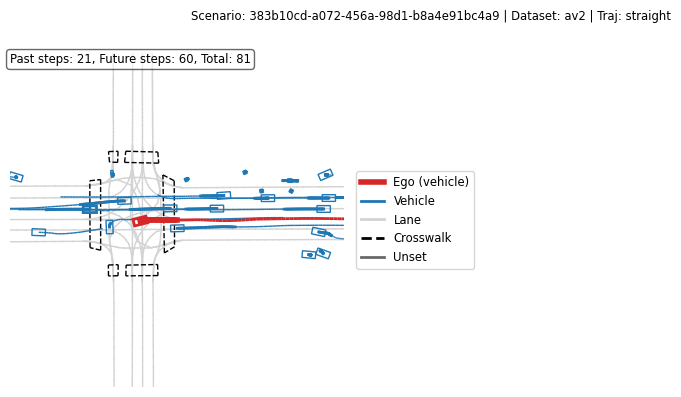
\includegraphics[width=\textwidth]{figures/plot_datasetitem.png}
    \caption{
        \textbf{Enhanced DatasetItem Visualization.} A comprehensive view of a processed scenario showing: (a) the center agent (ego vehicle) in red with its historical trajectory, (b) surrounding agents with their temporal information including velocity vectors and heading indicators, (c) high-definition map polylines with semantic classifications (lanes in blue, crosswalks in black dashed, boundaries in gray), and (d) agent interaction zones and proximity relationships. This visualization demonstrates the multi-modal nature of the standardized \texttt{DatasetItem} format, capturing spatial and temporal dynamics used for trajectory prediction tasks.
    }
    \label{fig:datasetitem_visualization}
\end{figure}

\newpage
\section{Model Architecture and Functional Decomposition}
\label{ch:model_architecture}

% \chapter{The Query-Centric Paradigm}
\label{chap:query_centric_paradigm}

\section{Motivation and Background}
Trajectory prediction for autonomous driving requires encoding both dynamic agents (vehicles, pedestrians) and static context (road lanes, traffic elements) into a representation suitable for forecasting future motion. Traditionally, the \emph{agent-centric} encoding scheme is used, where all coordinates are normalized with respect to a single reference agent (the prediction target). This normalizes the target agent to the origin and aligns its heading with the $x$-axis, simplifying learning for that agent. However, this approach has key drawbacks:
\begin{itemize}
    \item \textbf{Redundant computation:} Each time the prediction target changes (or time advances), the entire scene must be re-normalized and re-encoded.
    \item \textbf{Broken symmetry:} The encoding is tied to a particular agent, breaking permutation symmetry and complicating joint or multi-agent prediction.
\end{itemize}

Zhou et al.~\cite{Zhou2023QueryCentric} proposed the groundbreaking \textbf{query-centric paradigm}, where \emph{each scene element is encoded in its own local coordinate frame}. Every agent and every map element defines a ``query'' with its own origin and orientation, and features are expressed relative to that frame. This paradigm shift, implemented in QCNet and later extended in QCNeXt~\cite{qcnextZhou2023}, enables:
\begin{itemize}
    \item \textbf{Efficient reuse:} Encodings are independent of prediction target and can be shared across agents and time steps.
    \item \textbf{Permutation symmetry:} No agent is privileged; all elements are represented equally.
    \item \textbf{Multi-agent and streaming:} The same scene encoding can be used for parallel prediction of all agents and for streaming updates.
    \item \textbf{Joint prediction capability:} Unlike marginal prediction approaches, query-centric models can effectively capture future social interactions among agents.
\end{itemize}

\begin{figure}[t]
\centering
% (Placeholder) Illustration of agent-centric vs. query-centric reference frames in a driving scene.
\caption[Agent-centric vs. Query-centric Frames]{\textbf{Agent-centric vs. Query-centric representations.} \emph{Left:} Agent-centric scheme with the target agent at the origin and all others transformed. \emph{Right:} Query-centric scheme where each agent and map element uses its own local frame.}
\label{fig:agent_vs_query}
\end{figure}

\section{Coordinate Frames and Transformations}
\subsection{Agent-Centric Coordinate Transformation}
In the agent-centric paradigm, if $(x_{\text{ref}}, y_{\text{ref}}, \theta_{\text{ref}})$ is the reference agent's pose, any global point $(x, y)$ is transformed via:
\begin{equation}
\label{eq:agent_centric_transform}
\begin{pmatrix}
    x_{\text{rel}} \\ y_{\text{rel}}
\end{pmatrix}
=
\begin{pmatrix}
    \cos\theta_{\text{ref}} & \sin\theta_{\text{ref}} \\
    -\sin\theta_{\text{ref}} & \cos\theta_{\text{ref}}
\end{pmatrix}
\begin{pmatrix}
    x - x_{\text{ref}} \\ y - y_{\text{ref}}
\end{pmatrix}
\end{equation}
so that the reference agent is at $(0,0)$ and faces the $+x$ axis.

\subsection{Query-Centric Transformation}
In the query-centric paradigm, each element $e$ at $(x_e, y_e, \theta_e)$ defines its own frame. Any point $(x, y)$ is transformed via:
\begin{equation}
\label{eq:query_frame_transform}
\begin{pmatrix}
    x' \\ y'
\end{pmatrix}
=
\begin{pmatrix}
    \cos\theta_e & \sin\theta_e \\
    -\sin\theta_e & \cos\theta_e
\end{pmatrix}
\begin{pmatrix}
    x - x_e \\ y - y_e
\end{pmatrix}
\end{equation}
so that $e$ is at $(0,0)$ and oriented along $+x'$.

Each element is encoded in its own frame, and relative relationships between elements are preserved by computing relative positional embeddings during attention computation.

\section{Geometric Deep Learning Symmetries}
The query-centric paradigm is motivated by fundamental symmetries from geometric deep learning~\cite{bronstein2021geometric}:
\begin{itemize}
    \item \textbf{Permutation symmetry:} The set of agents and map elements is unordered. The model should be equivariant to permutations of the input.
    \item \textbf{$\SE(2)$ symmetry:} The laws of physics are invariant under translation and rotation. The model should be equivariant to global $\SE(2)$ transformations.
    \item \textbf{Temporal symmetry:} The encoding should be invariant to shifts in the time origin (for streaming).
\end{itemize}

Query-centric encoding naturally respects these symmetries as demonstrated in QCNet~\cite{Zhou2023QueryCentric}:
\begin{itemize}
    \item Each element is encoded independently, supporting permutation-equivariant processing through Transformer architectures.
    \item Local frames remove dependence on global position/orientation, so encodings are invariant to global $\SE(2)$ transforms.
    \item Static elements (map lanes) need not be re-encoded over time; dynamic elements can be incrementally updated, enabling streaming processing.
\end{itemize}

This approach follows the philosophy of \emph{relative spacetime}, where the model is equipped with roto-translation invariance in the space dimension and translation invariance in the time dimension. These invariance properties not only enable accurate multi-agent forecasting fundamentally but also empower the encoder with streaming processing capabilities~\cite{qcnextZhou2023}.

\section{Polar Encodings and Relative Descriptors}
\subsection{Static Map Segments}
Each lane polyline is broken into straight segments between consecutive points $(x_s, y_s)$ and $(x_e, y_e)$. The segment's orientation is
\begin{equation}
\phi = \arctan2(y_e - y_s,\, x_e - x_s)
\end{equation}
and its length is
\begin{equation}
L = \sqrt{(x_e - x_s)^2 + (y_e - y_s)^2}
\end{equation}
In the segment's own frame (origin at $(x_s, y_s)$, $x'$ axis along the segment), the start is at $(0,0)$ and the end is at $(L,0)$. The geometric feature for the segment is simply $L$ (plus semantic attributes).

\subsection{Dynamic Agent Motions}
For each agent $j$ at time $t$, with pose $(x_{j,t}, y_{j,t}, \theta_{j,t})$, the displacement to $t+1$ is
\begin{equation}
\Delta x_{j,t} = x_{j,t+1} - x_{j,t}, \qquad \Delta y_{j,t} = y_{j,t+1} - y_{j,t}
\end{equation}
Rotated into the agent's frame at $t$:
\begin{equation}
\begin{pmatrix}
    \Delta x'_{j,t} \\ \Delta y'_{j,t}
\end{pmatrix}
=
\begin{pmatrix}
    \cos\theta_{j,t} & \sin\theta_{j,t} \\
    -\sin\theta_{j,t} & \cos\theta_{j,t}
\end{pmatrix}
\begin{pmatrix}
    \Delta x_{j,t} \\ \Delta y_{j,t}
\end{pmatrix}
\end{equation}
The polar encoding is:
\begin{align}
l_{j,t} &= \sqrt{(\Delta x'_{j,t})^2 + (\Delta y'_{j,t})^2} \\
\delta\theta_{j,t} &= \arctan2(\Delta y'_{j,t},\, \Delta x'_{j,t})
\end{align}
where $l_{j,t}$ is the motion length (distance traveled) and $\delta\theta_{j,t}$ is the change in direction relative to heading.

\subsection{Relative Positional Descriptors}
To relate elements $i$ and $j$, QCNet~\cite{Zhou2023QueryCentric} defines the following relative descriptor:
\begin{equation}
\label{eq:relative_descriptor_v2}
d_{j \to i} = \left(
    \left\| p_j - p_i \right\|,\;
    \arctan2(y_j - y_i,\, x_j - x_i) - \theta_i,\;
    \theta_j - \theta_i,\;
    t_j - t_i
\right)
\end{equation}
where $p_i = (x_i, y_i)$, $\theta_i$ is orientation, $t_i$ is timestamp. This encodes:
\begin{itemize}
    \item Euclidean distance between $i$ and $j$
    \item Relative direction from $i$ to $j$ in $i$'s frame
    \item Orientation difference
    \item Time difference
\end{itemize}
These are typically embedded using Fourier features and MLPs to produce relative embedding vectors used in attention layers, specifically in the key/value elements that are concatenated with spatial-temporal positional embeddings relative to the query elements before performing QKV attention.

\begin{figure}[t]
\centering
% (Placeholder) Diagram of query-centric encoding pipeline.
\caption[Query-Centric Encoding Pipeline]{\textbf{Query-centric encoding pipeline.} Raw scene data is transformed into local frames for each element, embedded as features, and paired with relative descriptors for use in a permutation- and $\SE(2)$-equivariant encoder.}
\label{fig:query_pipeline}
\end{figure}

\section{QCNet Architecture and Multi-Agent Extensions}

\subsection{Factorized Attention-Based Scene Encoder}
The query-centric scene encoder in QCNet~\cite{Zhou2023QueryCentric} employs a factorized attention-based Transformer that captures temporal dependencies, agent-map interactions, and social interactions. The architecture follows a systematic attention pattern:

\begin{enumerate}
    \item \textbf{Map-Map Attention:} Captures spatial relationships between static map elements (lanes, crosswalks, etc.)
    \item \textbf{Temporal Attention:} Models temporal dependencies within each agent's trajectory history
    \item \textbf{Agent-Map Attention:} Encodes interactions between dynamic agents and static map context
    \item \textbf{Social Attention:} Captures social interactions among agents at historical time steps
\end{enumerate}

The encoder produces map encodings of shape $[M, D]$ and agent encodings of shape $[A, T, D]$, where $M$, $A$, $T$, $D$ are the numbers of map polygons, modeled agents, historical time steps, and hidden units, respectively.

\subsection{From Marginal to Joint Prediction: QCNeXt}
While QCNet excels at marginal trajectory prediction (predicting each agent independently), real-world driving scenarios require modeling future social interactions. QCNeXt~\cite{qcnextZhou2023} extends the query-centric paradigm to joint multi-agent trajectory prediction through several key innovations:

\subsubsection{Multi-Agent DETR-Like Decoder}
QCNeXt introduces a novel decoder architecture that can capture future social interactions among agents:

\begin{itemize}
    \item \textbf{Anchor-Free Trajectory Proposal:} Uses $K$ randomly initialized embeddings, each repeated $A$ times to form a tensor of shape $[K, A, D]$, where each row represents one of the $K$ joint futures.
    \item \textbf{Mode2Time Cross-Attention:} Updates embeddings to assign responsibility for predicting each agent.
    \item \textbf{Mode2Map Cross-Attention:} Incorporates neighboring map information.
    \item \textbf{Row-wise Self-Attention:} Models social interactions among agents within each joint scene.
    \item \textbf{Column-wise Self-Attention:} Enables communication between the $K$ joint scenes.
\end{itemize}

\subsubsection{Scene-Level Scoring}
Unlike agent-level scoring in marginal prediction, QCNeXt employs scene-level confidence scoring using attentive pooling to summarize all target agents' mode embeddings into a single scene embedding, acknowledging that some agents may have uninteresting behavior (e.g., remaining static).

\subsubsection{Joint Distribution Modeling}
The joint future trajectory distribution is parameterized as a mixture of Laplace distributions:
\begin{equation}
\sum_{k=1}^K \pi_{k} \prod_{i=1}^{A'} \prod_{t=1}^{T'} f\left(\mathbf{p}_i^{t,x} \mid \boldsymbol{\mu}_{i,k}^{t,x}, \mathbf{b}_{i,k}^{t,x}\right) f\left(\mathbf{p}_i^{t,y} \mid \boldsymbol{\mu}_{i,k}^{t,y}, \mathbf{b}_{i,k}^{t,y}\right)
\end{equation}
where $K$ is the number of modes, $A'$ is the number of target agents, and $T'$ is the prediction horizon.

\subsection{Performance Breakthrough}
Remarkably, QCNeXt demonstrated that a joint prediction model can outperform marginal prediction models even on marginal metrics, challenging the previous belief that joint prediction was inherently more difficult. This breakthrough won the championship of the Argoverse Challenge at CVPR 2023 Workshop on Autonomous Driving, achieving state-of-the-art results on the Argoverse 2 multi-agent motion forecasting benchmark~\cite{av2Wilson2023}.

\section{Algorithm: Query-Centric Conversion}
\subsection*{Conversion from DatasetItem to QCDatasetItem}
We describe the process for converting a standard dataset item (with global or agent-centric coordinates) into a query-centric dataset item. The pseudocode uses the following structures:
\begin{itemize}
    \item \texttt{MapPolylines}: List of polylines (each a sequence of global points)
    \item \texttt{AgentTrajectories}: List of agents, each with a sequence of $(x, y, \theta)$ states over time
    \item \texttt{QCDatasetItem}: Holds two lists: lane segments (with query-centric features) and agent motion vectors (with query-centric features)
\end{itemize}

\begin{algorithm}[h!]
\caption{Convert DatasetItem (global/agent-centric) to QCDatasetItem (query-centric)}
\label{alg:qc_conversion}
\begin{algorithmic}[1]
\REQUIRE \texttt{item} = (\texttt{MapPolylines}, \texttt{AgentTrajectories}, \texttt{TargetAgents})
\ENSURE \texttt{qc\_item} = (\texttt{SegmentList}, \texttt{MotionList})

\COMMENT{Process static context (map lanes)}
\STATE Initialize empty \texttt{SegmentList}
\FOR{polyline $P$ in \texttt{item.MapPolylines}}
    \FOR{consecutive pair $(p_k, p_{k+1})$ in $P$}
        \STATE $(x_s, y_s) \gets p_k$; $(x_e, y_e) \gets p_{k+1}$
        \STATE $\Delta x \gets x_e - x_s$; $\Delta y \gets y_e - y_s$
        \STATE $\phi \gets \arctan2(\Delta y, \Delta x)$
        \STATE $L \gets \sqrt{\Delta x^2 + \Delta y^2}$
        \STATE $m_{\text{seg}} \gets [L,\; \text{lane\_type}(P),\; \text{other attributes}]$
        \STATE Append $m_{\text{seg}}$ to \texttt{SegmentList}
    \ENDFOR
\ENDFOR

\COMMENT{Process dynamic context (agents)}
\STATE Initialize empty \texttt{MotionList}
\FOR{agent $j$ in \texttt{item.AgentTrajectories}}
    \STATE Extract trajectory states $(x_{j,t}, y_{j,t}, \theta_{j,t})$ for $t = t_0 - T_p$ to $t_0$
    \FOR{$t = t_0 - T_p$ to $t_0 - 1$}
        \STATE $\Delta x \gets x_{j,t+1} - x_{j,t}$; $\Delta y \gets y_{j,t+1} - y_{j,t}$
        \STATE $\psi \gets \theta_{j,t}$
        \COMMENT{Rotate displacement into agent's local frame}
        \STATE $\begin{pmatrix}\Delta x',\, \Delta y'\end{pmatrix} \gets
        \begin{pmatrix}
            \cos\psi & \sin\psi \\
            -\sin\psi & \cos\psi
        \end{pmatrix}
        \begin{pmatrix}
            \Delta x \\ \Delta y
        \end{pmatrix}$
        \STATE $l \gets \sqrt{(\Delta x')^2 + (\Delta y')^2}$
        \STATE $\delta\theta \gets \arctan2(\Delta y',\, \Delta x')$
        \STATE $m_{\text{mot}} \gets [l,\, \delta\theta,\, \text{agent\_type}(j),\, \text{other attributes}]$
        \STATE Append $m_{\text{mot}}$ to \texttt{MotionList}
    \ENDFOR
\ENDFOR
\RETURN \texttt{qc\_item} = (\texttt{SegmentList}, \texttt{MotionList})
\end{algorithmic}
\end{algorithm}

\subsection*{Algorithm Details}
The static context loop iterates over each polyline and its segments, computing length and attributes for each segment in its own local coordinate frame. The dynamic context loop processes each agent's historical trajectory, computes motion vectors, and rotates them into the agent's heading frame, producing polar features as described in QCNet~\cite{Zhou2023QueryCentric}. Additional attributes such as agent type, velocity, and acceleration may be concatenated to enhance the representation.

Optionally, the origin and orientation for each element can be stored for later reconstruction of global coordinates during inference. Relative descriptors $d_{j \to i}$ (Eq.~\eqref{eq:relative_descriptor_v2}) are typically computed on-the-fly during model forward passes and embedded using learnable functions, not stored in the dataset.

This conversion process is fundamental to enabling the query-centric paradigm's benefits, including permutation equivariance, streaming processing capabilities, and efficient multi-agent reasoning as demonstrated in both QCNet~\cite{Zhou2023QueryCentric} and its joint prediction extension QCNeXt~\cite{qcnextZhou2023}.

\section{Discussion: Expressiveness and Equivariance}
Query-centric encoding achieves several important properties that make it superior to traditional agent-centric approaches:

\begin{itemize}
    \item \textbf{Expressiveness:} Each element's representation is a learnable summary of its local geometry and context. The model can capture complex interactions via attention over both content and relative pose.
    \item \textbf{Permutation- and $\SE(2)$-equivariance:} The encoding respects symmetries of the scene, enabling generalization and reducing the need for data augmentation.
    \item \textbf{Inductive bias and model simplicity:} By removing dependence on global coordinates, standard architectures (MLPs, Transformers) suffice, without specialized equivariant layers.
    \item \textbf{Multi-agent and streaming capabilities:} All agents and map elements share a common latent space, supporting joint reasoning and efficient updates.
    \item \textbf{Scalability:} The paradigm enables training on large-scale datasets like Argoverse 2~\cite{av2Wilson2023}, Waymo Open Motion Dataset~\cite{wmodSun2020}, and ScenarioNet~\cite{scenarionetLi2023}.
\end{itemize}

The success of query-centric models has influenced subsequent trajectory prediction architectures, including UniTraj~\cite{unitrajFeng2024} and LMFormer~\cite{lmformerYadav2025}, demonstrating the paradigm's broad applicability and impact on the field.

\section{Integration with Modern Architectures}
The query-centric paradigm has been successfully integrated with various modern deep learning architectures:

\begin{itemize}
    \item \textbf{Transformer-based models:} QCNet and QCNeXt demonstrate the natural synergy between query-centric encoding and attention mechanisms.
    \item \textbf{Graph neural networks:} The paradigm can be adapted for GNN-based trajectory prediction by treating each element's local frame as a node feature.
    \item \textbf{Diffusion models:} Recent work has explored combining query-centric representations with diffusion-based trajectory generation.
    \item \textbf{Multi-modal architectures:} The encoding scheme facilitates integration with camera and LiDAR data through consistent spatial representations.
\end{itemize}

In summary, the query-centric paradigm provides a principled, symmetry-respecting, and efficient foundation for trajectory forecasting. The combination of local polar encodings and relative descriptors yields a flexible and lossless representation, underpinning the success of recent state-of-the-art models. This approach has fundamentally changed how the community thinks about scene representation for autonomous driving, moving from agent-centric to truly democratic, multi-agent reasoning systems.
\subsection{Context-Aware Scene Prediction}
\label{ssec:caspnet}

This section distills the key ideas behind \emph{Context-Aware Scene Prediction Network} (CASPNet)~\cite{caspnetSchäfer2022} and its transformer successor \emph{CASPFormer}~\cite{caspformerYadav2024}. Both architectures perform \emph{joint multi-agent} trajectory forecasting from rasterized bird's-eye-view (BEV) inputs, yet they differ strongly in how they fuse context and decode trajectories. We summarize their core components, strengths, and limitations.

\subsubsection*{CASPNet: Rasterized BEV Encoding with Dual FPN}

\textbf{CASPNet}~\cite{caspnetSchäfer2022} processes rasterized BEV inputs through a dual-encoder architecture that separately handles dynamic agent trajectories and static HD map information. Overall, it strongly resembles a \emph{fully convolutional network} as it employs no fully connected layers, meaning that the spatial representation of the scene is preserved throughout the network. Furthermore, it can be classified as a \emph{feature pyramid network} (FPN)~\cite{FPNLin2017} as it provides the decoder with latent representations at multiple spatial resolutions. Together, these architectural qualities starkly resemble the famous \emph{U-Net} architecture with \emph{lateral skip connections}~\cite{UNetLSRonneberger2015}. Considering CASPNet's usage of \emph{attention} mechanisms within the skip connections its closest relative in the field of image segmentation is the \emph{Attention U-Net}~\cite{UNetAttnOktay2018}.

\begin{figure}[ht]
  \centering
  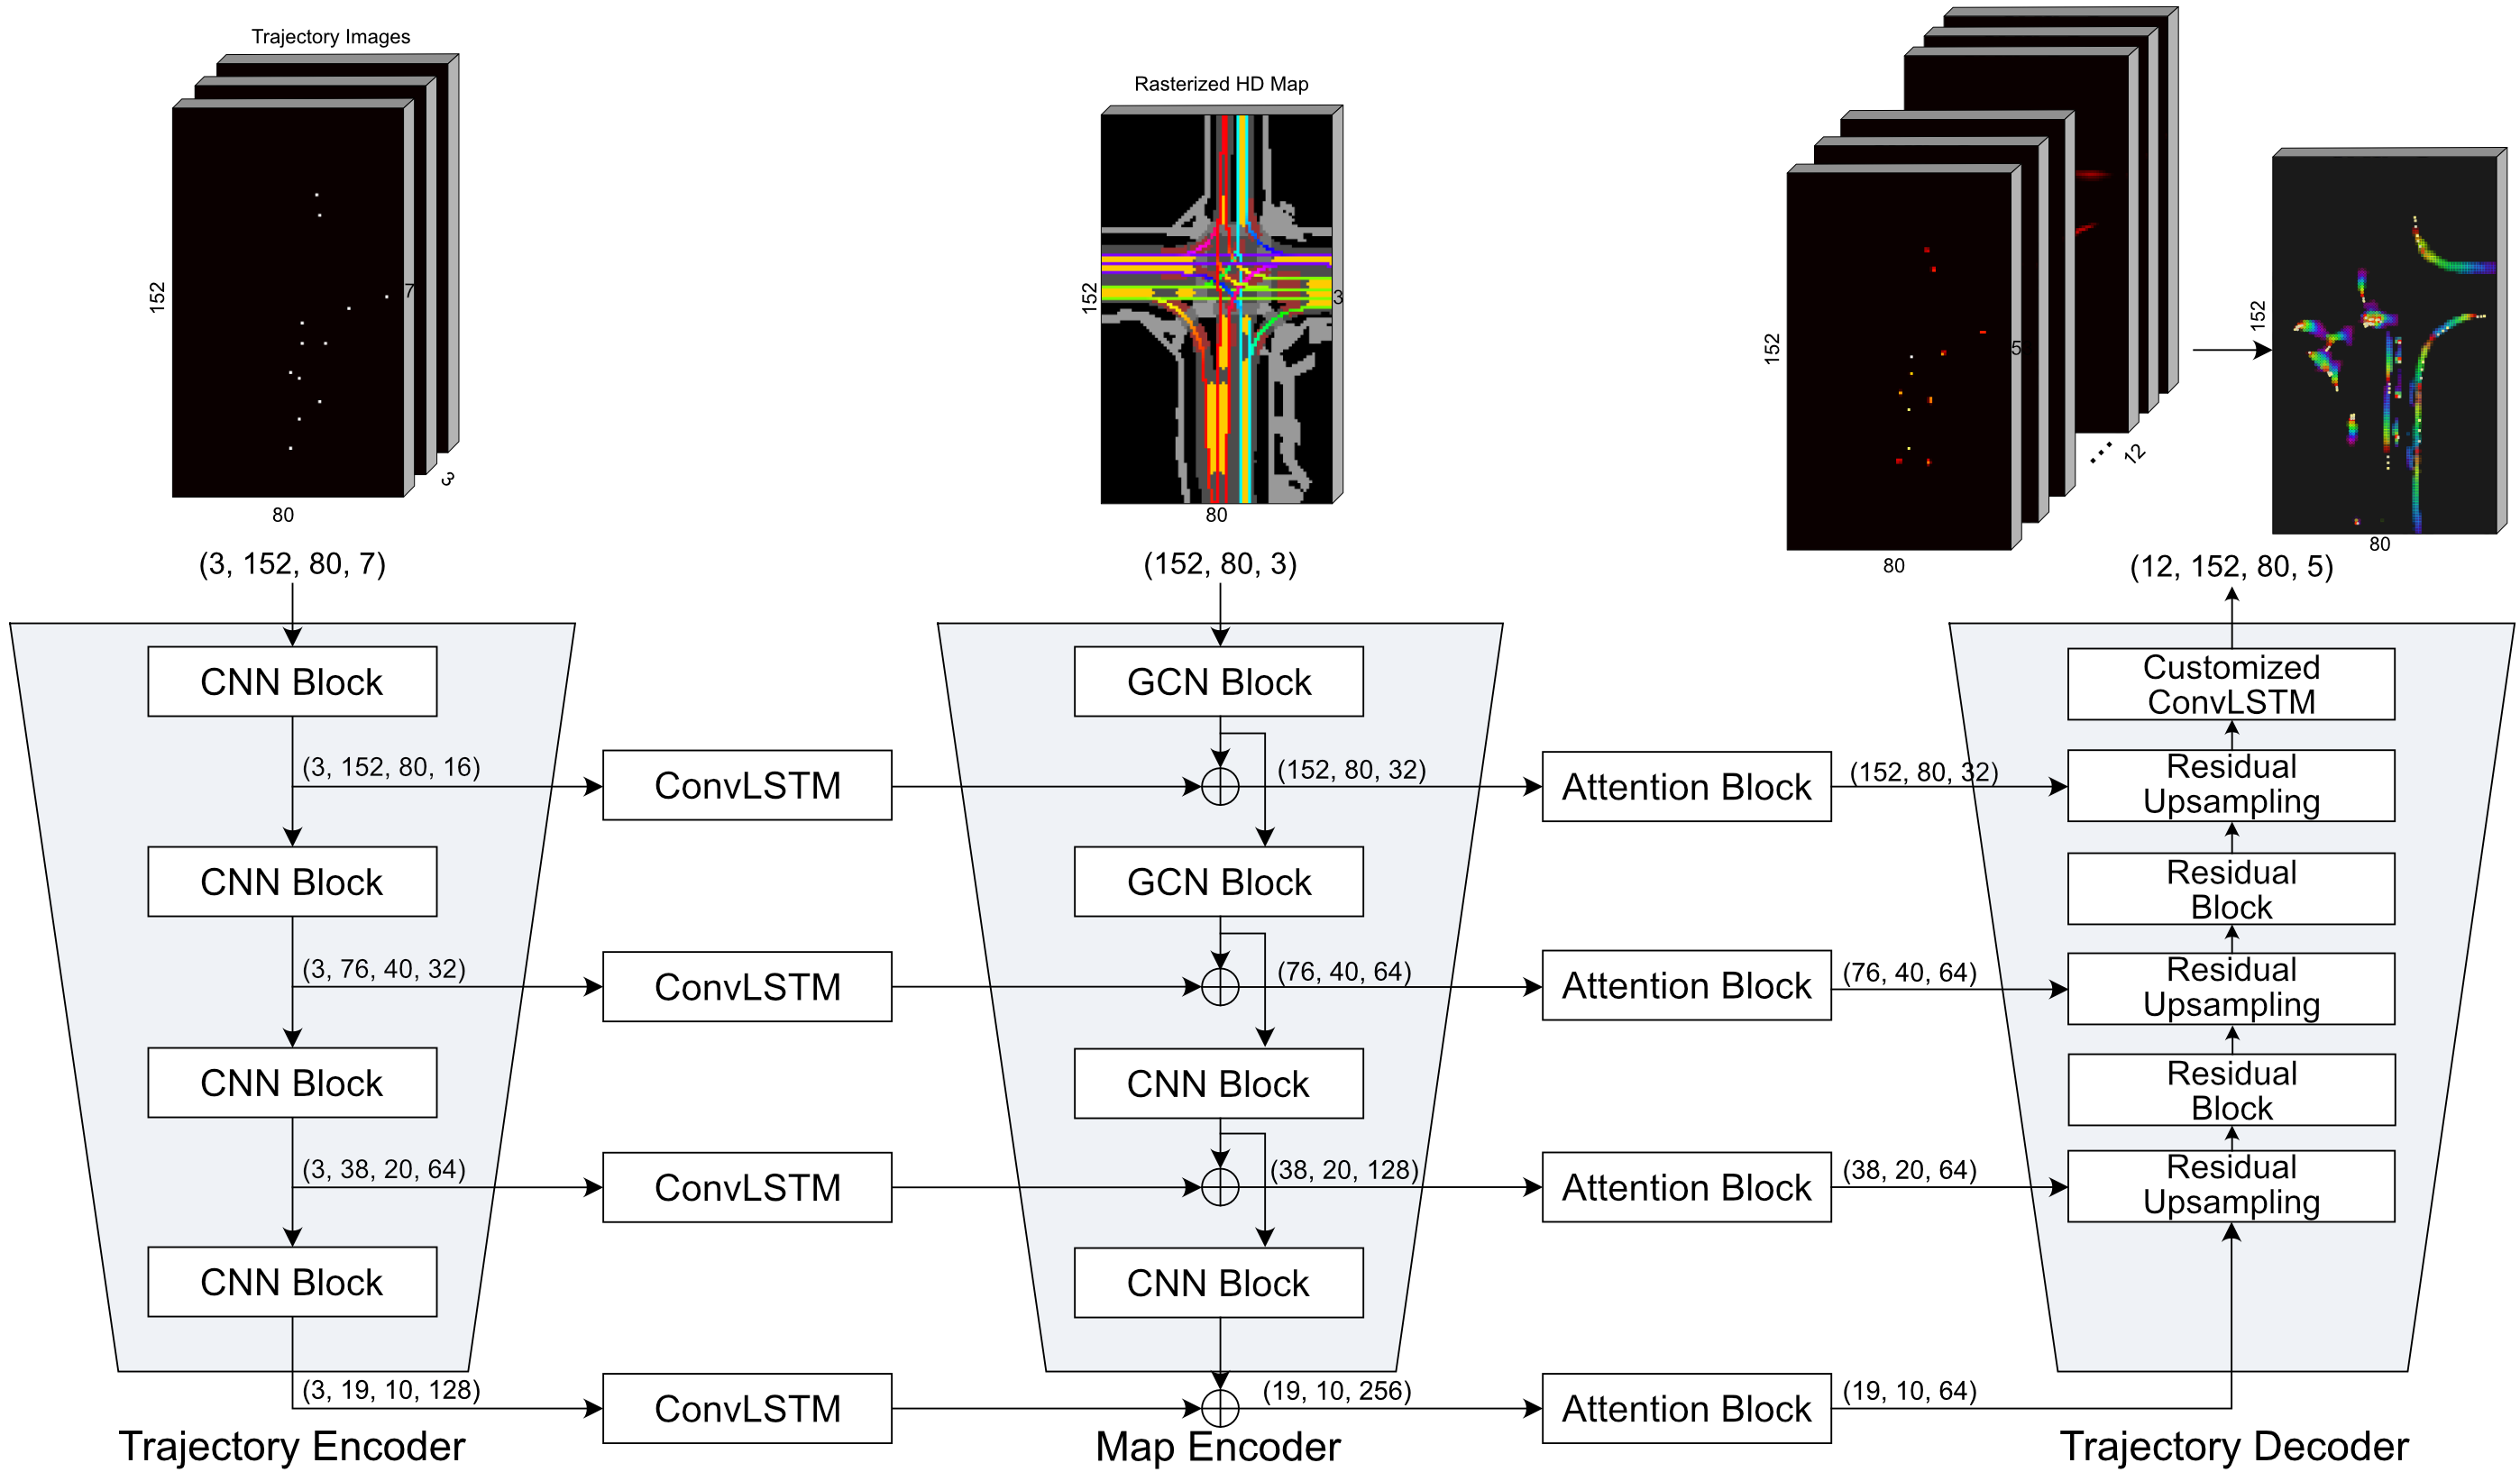
\includegraphics[width=\linewidth]{figures/caspnet_arch.png}
  \caption{CASPNet architecture overview: dual FPN encoders with Gabor filters, pixel-adaptive attention, and grid-based ConvLSTM decoder~\cite{caspnetSchäfer2022}.}
  \label{fig:caspnet_overview}
\end{figure}

The CASPNet architecture is illustrated in~\autoref{fig:caspnet_overview} and consists of the following components:
\begin{description}[leftmargin=1em,itemsep=2pt]
\item[Dual FPN encoders.] Separate feature-pyramid networks process
\begin{enumerate}[label=\roman*)]
    \item a BEV stack of past agent trajectories \( \mathbf{I}_d\in\R^{T_p\times H\times W\times F_d} \)
    \item a static HD-map raster \( \mathbf{I}_s\in\R^{H\times W\times F_s} \)
\end{enumerate}

At each level \( \ell \), the trajectory branch produces:
\begin{equation}
\label{eq:fpn_traj}
\mathbf{F}^{\mathrm{traj}}_{\ell}(t) = \mathrm{CNN}_\ell\bigl(\mathbf{I}_{d}(t)\bigr) \in \R^{T_p \times C_\ell \times H_\ell \times W_\ell}
\end{equation}
where all \( T_p \) BEV frames representing the agent trajectories are encoded independently by the same CNN, yielding a \emph{time-dependent} \emph{multi-scale feature map} \( F^{\mathrm{traj}}_{\ell}(t) \in \R^{C_\ell \times H_\ell \times W_\ell} \) at each pyramid level \(\ell\) and timestep \( t \in \{0,\dots,T_p - 1\} \).\\

The static map branch employs \emph{steerable Gabor filters}%
\footnote{See~\autoref{ssec:gabor_filters} for further details.}
in the first two convolutional blocks. These filters are particularly well-suited for capturing orientation and scale-sensitive features like road networks, where lane markings exhibit strong orientation and scale-specific patterns. A Gabor filter combines a Gaussian envelope with a sinusoidal carrier wave, allowing it to simultaneously localize features in space and frequency. This makes it highly effective for detecting elongated and parallel structures across varying scales and rotations~\cite{steerableGaborFilters}.\\
The map features are computed as follows:
\begin{equation}
\label{eq:fpn_map}
\mathbf{F}_{\ell}^{\mathrm{map}}
= \mathrm{CNN}_\ell^{\circ}(\mathbf{I}_s) \in \R^{C_\ell \times H_\ell \times W_\ell},
\end{equation}

\item[Temporal fusion.] ConvLSTM cells at every pyramid level aggregate the temporal context across all \(T_p\) timesteps yielding a single feature map per level~\cite{shi2015ConvLSTM}:
\begin{equation}
\label{eq:fpn_fusion_traj}
\mathbf{F}_{\ell}^{\mathrm{traj}}
= \mathrm{ConvLSTM}_\ell\Bigl\{\mathbf{F}^{\ell}_{d}(t)\Bigr\}_{t=1}^{T_p} \in \R^{C_\ell \times H_\ell \times W_\ell},
\end{equation}
which are then concatenated with the static map features at each level:
\begin{equation}
\label{eq:fpn_fusion}
\boldsymbol{\mathcal{F}}=\{\mathbf{F}_\ell^{\mathrm{traj}}\oplus \mathbf{F}_\ell^{\mathrm{map}}\}_{\ell=0}^{L_{\text{FPN}}-1}, \quad \text{where } \mathbf{F}_\ell \in \R^{2 C_\ell \times H_\ell \times W_\ell}
\end{equation}
\( \boldsymbol{\mathcal{F}} \) is the resulting latent feature pyramid.

\item[Pixel-adaptive attention.] The \emph{Attention Block} in the lateral skip connections (\autoref{fig:caspnet_overview}) adaptively blends the receptive fields of multiple \emph{dilated convolutions}~\cite{dilatedConv21} per spatial location, capturing multi-scale interactions through learned per-pixel attention weights over different dilation rates, similar to~\cite{UNetAttnOktay2018}. For each location \((i,j)\) at pyramid level \(\ell\), the mechanism computes:
\begin{equation}
\label{eq:pixel_attention}
\mathbf{F}_{\ell}^{(i,j)} = \sum_{r} \alpha^{(i,j)}_{r} \cdot \text{DilatedConv}_r(\mathbf{F}^{(i,j)}_{\ell}),
\end{equation}
where \(\alpha^{(i,j)}_{r} = \text{softmax}(\text{Conv}(\mathbf{F}^{(i,j)}_{\ell}))\) are learned attention weights that dynamically select appropriate receptive field sizes for each spatial location.

\item[Grid-based decoder.] The decoder employs a series of \emph{residual up-sampling blocks} to progressively up-sample the feature maps from the FPN to the original raster resolution. Each residual block consists of a parallel \emph{transposed convolution} and a \emph{linear interpolation} layer. The resulting feature maps of each up-sampling block are concatenated with the corresponding feature maps the next level of the FPN.\\
Finally, the decoder uses a \emph{ConvLSTM} layer to autoregressively generate future predictions. For each future timestep \(t \in \{T_p, \ldots, T_p + T_f - 1\}\), the decoder outputs a occupancy probabilities and motion offsets. The occupancy probabilities are represented as a categorical distribution over the possible agent classes at each pixel, while the motion offsets represent the displacement of each pixel with respect to the previous timestep~\cite{caspnetSchäfer2022}.

\paragraph{Pros.} Inference time independent of agent count; inherent multi-modality via heat-map superposition; good interpretability through adaptation of well-established motifs from the field of image segmentation.
\paragraph{Cons.} Metric accuracy capped by raster resolution; inference cost scales with grid size; vectorized outputs require post-processing; no \emph{explicit} prediction of \( M \) multi-modal; doesn't respect identities of agents; limited temporal modeling; no explicit relationship modeling between agents or between agents and map; no symmetries in the agent-centric coordinate system for all but the ego agent; only suited for \emph{single-agent} motion forecasting.

The follow-up work CASPNet++~\cite{caspnetppSchäfer2023} improves upon CASPNet by replacing its single heat-map head with a two-stage design to capture spatio-temporal occupancy grids for every actor, as well as an Agent decoder that transforms the grid cells of selected targets into explicit, multi-modal trajectory splines, thereby modelling interactions more richly and introducing the ability to predict \( M \) explicit multi-modal trajectories. However, while CASPNet++ improves upon the original architecture in terms of accuracy and interaction modeling and allows for \emph{true} joint multi-agent forecasts, we will not discuss it in detail.

%--------------------------------------------------------------------
%% Above is done %%
\subsubsection*{CASPFormer: Hybrid CNN-Transformer with Deformable Attention}
\label{ssec:caspformer}

\textbf{CASPFormer}~\cite{caspformerYadav2024} retains CASPNet's, FPN-CNN backbone while replacing its grid-based decoder with a transformer that emits vectorized \((x,y)\) trajectories, explicitly modeling the uncertainties of each mode as a \emph{parametrized Laplacian}. The core innovation lies in adapting \emph{deformable attention}~\cite{zhu2021deformabledetr} from object detection to trajectory prediction, enabling sparse, efficient attention over multi-scale feature representations. The overall architecture is illustrated in~\autoref{fig:caspformer_overall}, with the detailed decoder mechanism shown in~\autoref{fig:caspformer_decoder}. The following section requires basic understanding of both regular and deformable attention mechanisms. While we are referring the reader to~\cite{vaswani2023attention} and~\cite{zhu2021deformabledetr} for a detailed introduction, a concise explanation of the key concepts is provided in \autoref{sec:deformable_attention}.

\begin{figure}[ht]
  \centering
  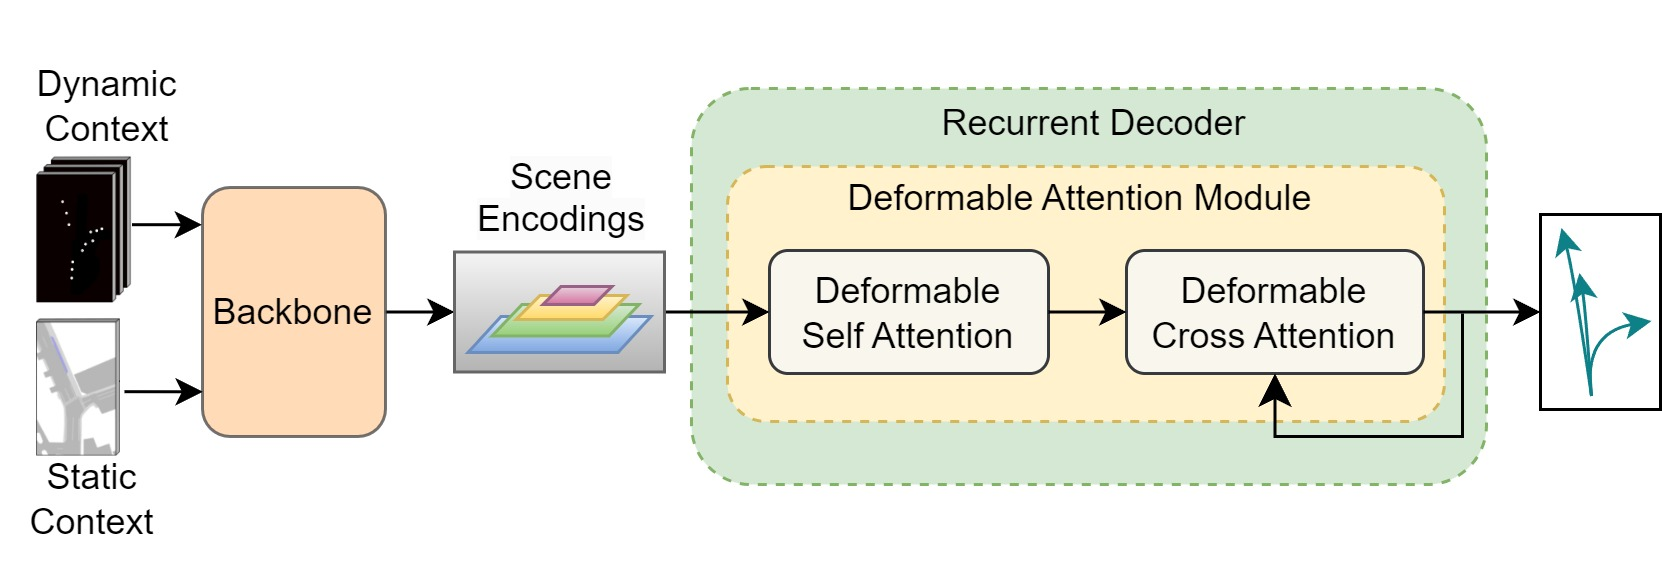
\includegraphics[width=\linewidth]{figures/caspformer-overall-arch.jpg}
  \caption{CASPFormer overall architecture: CNN+FPN backbone processes rasterized BEV inputs, deformable self-attention fuses multi-scale features, and recurrent deformable cross-attention autoregressively decodes vectorized trajectories~\cite{caspformerYadav2024}.}
  \label{fig:caspformer_overall}
\end{figure}

\begin{figure}[ht]
  \centering
  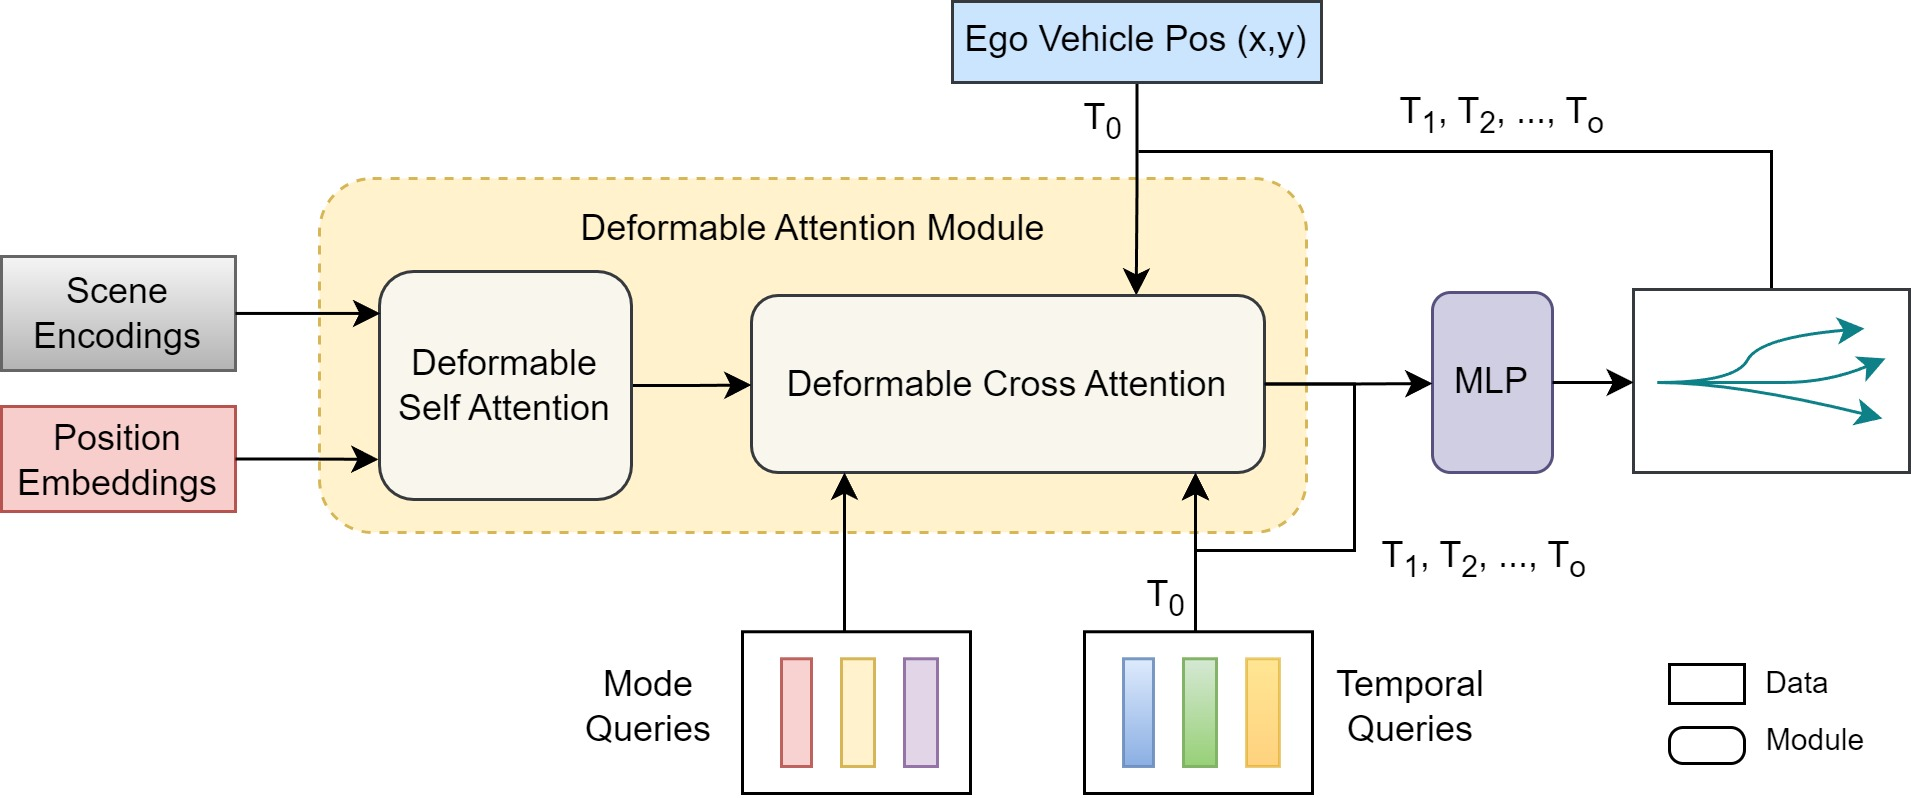
\includegraphics[width=0.85\linewidth]{figures/caspformer_decoder.jpg}
  \caption{CASPFormer decoder architecture with temporal and mode queries, deformable cross-attention, and autoregressive trajectory generation~\cite{caspformerYadav2024}.}
  \label{fig:caspformer_decoder}
\end{figure}

The CASPFormer as depicted in \autoref{fig:caspformer_decoder} decoder consists of the following key components:

\begin{description}[leftmargin=1em,itemsep=2pt]
\item[Multi-Scale Deformable Self-Attention (MSDA).] The FPN feature maps \(\boldsymbol{\mathcal{F}} = \{\mathbf{F}_\ell\}_{\ell=0}^{L-1}\) as previously defined in \autoref{eq:fpn_fusion} are first flattened and enriched with non-learnable 2D sinusoidal positional encodings as introduced in~\cite{vaswani2023attention} to preserve spatial relationships across different scales. MSDA performs feature fusion by allowing each spatial location to attend to relevant features across all pyramid levels:

\begin{equation}
\label{eq:msda_operation}
\mathbf{Z}^{\text{SA}} = \sum_{n=1}^{N_H} \mathbf{W}_{n} \left[\sum_{\ell=0}^{L_{\text{FPN}}-1} \sum_{k=1}^{K_s} A_{n\ell qk} \cdot \mathbf{F}_\ell(\phi_{\ell}(\mathbf{p}_q) + \boldsymbol{\Delta p}_{n\ell qk}) \right]
\end{equation}

Here, \emph{queries} and \emph{keys} are derived from the same flattened feature maps \(\text{Flatten}(\boldsymbol{\mathcal{F}} + \textbf{PE})\). The learned offsets \(\boldsymbol{\Delta p}_{\ell nkq} \in \R^2\) enable each query to attend to informative locations across the entire feature pyramid, while being constrained to all features of the n-th attention head. \( \phi_{\ell} \) re-scales the normalized coordinates \( \mathbf{p}_q \in [0,1]^2\) to the spatial dimensions of the feature map at level \(\ell\).\\
  The output of the MSDA is a latent representation of the entire scene, encoding all spatio-temproal and social dynamics of the agents and the map. Hence, this module should be seen as part of the scene-encoder, rather than the decoder.

\item[Recurrent Deformable Cross-Attention.] The fused features \(\mathbf{Z}^{\text{SA}}\) serve as \emph{keys} and \emph{values} for the cross-attention mechanism. CASPFormer employs a dual-query approach that combines \emph{temporal queries} and \emph{mode queries} to capture both temporal dependencies and facilitate mode diversity. The query construction is defined as:

\begin{equation}
\label{eq:dual_query_construction}
\begin{aligned}
\mathbf{Q}_t^{\text{temp}} &= \mathbbm{1}(t=T_p) \cdot \mathbf{E}_{\text{init}} + \mathbbm{1}(t>T_p) \cdot \mathbf{Z}^{\text{CA}}_{t-1} \\
\mathbf{Q}^{mode} &\in \R^{M \times d} \quad \text{(learnable mode embeddings)} \\
\mathbf{Q}_t &= \mathbf{Q}_t^{temp} \oplus \mathbf{Q}^{mode} \quad \text{(concatenated dual queries)}
\end{aligned}
\end{equation}

The temporal queries maintain temporal coherence across timesteps, while mode queries provide fixed embeddings to promote behavioral diversity and mitigate mode collapse.

For each timestep \(t\), the deformable cross-attention decoder updates the reference point \(\mathbf{p}^{ref}\) as the last position of the ego-vehicle \( \hat{\boldsymbol{\mu}}_{t-1}\) based on previous predictions and computes:
\begin{equation}
\label{eq:cross_attention_operation}
\mathbf{Z}^{\text{CA}}_t = \sum_{m=1}^{M} \mathbf{W}_m \left[ \sum_{k=1}^{K_s} A_{nkq} \cdot \mathbf{Z}^{\text{CA}}(\mathbf{p}^{ref} + \boldsymbol{\Delta p}_{nkq}) \right]
\end{equation}

where both the attention weights and offsets are computed as delineated in~\autoref{sec:deformable_attention}. The DCA block depicted in~\autoref{fig:caspformer_decoder} stacks three deformable cross-attention layers, each with its own set of learnable parameters, to refine the predictions iteratively. This allows the model to capture complex interactions and dependencies across multiple timesteps and modes.

\item[Autoregressive Decoding with Mixture Outputs.] The outputs of the final cross-attention layer are processed by an MLP to generate trajectory distributions as mixtures of Laplacian components:
\begin{equation}
\label{eq:mixture_trajectory_output}
\begin{aligned}
\hat{\boldsymbol{\mu}}_{t}, \hat{\mathbf{b}}_{t} &= \text{MLP}(\mathbf{Z}^{\text{CA}}_t)\\
\hat{\boldsymbol{\pi}} &= \text{softmax}(\text{MLP}(\mathbf{Z}^{\text{CA}}_t)) \\
\end{aligned}
\end{equation}
where \(\hat{\boldsymbol{\mu}}_{t} \in \R^{N_c \times M \times 2}\) are Cartesian position means, \(\hat{\mathbf{b}}_{t} \in \R^{N_c \times M \times 2}\) are uncertainty scales, and \(\hat{\boldsymbol{\pi}}_t \in \R^{N_c \times M}\) are mode probabilities for each of the \(M\) trajectory modes and each agent of interest; \( N_c \) being the number of agents in the scene, whose trajectories are to be predicted.

The recurrent architecture updates both the temporal queries and reference point at each timestep:
\begin{equation}
\label{eq:recurrent_updates}
\begin{aligned}
\mathbf{p}^{ref}_{(t+1)} &= \text{argmax}_m \hat{\boldsymbol{\pi}}_{t,ego} \cdot \hat{\boldsymbol{\mu}}_{t,m^{ego}} \\
\end{aligned}
\end{equation}
where \(m^* = \text{argmax}_m \hat{\boldsymbol{\pi}}_{t,ego}\) yields the index of the ego agent's most probable mode, hence the next reference point is set the likeliest predicted position of the ego vehicle (which must be one of the \( N_c \) agents of interest).
\end{description}

\paragraph{Loss Formulation and Training Recipe.} CASPFormer adopts the HiVT loss formulation~\cite{zhou2022hivt}, combining regression and classification objectives \(\mathcal{L} = \mathcal{L}_{reg} + \mathcal{L}_{cls}\) to optimize the predicted mixture of Laplacians.
To avoid numerical instability and mode collapse in mixture model optimization~\cite{rupprecht2017learning}, the regression loss adopts winner-takes-all (WTA) strategy, where only the mode with the lowest Euclidean distance to the ground truth trajectory is considered:
\begin{equation}
  \label{eq:caspformer_regression_loss}
  \mathcal{L}_{reg} = -\frac{1}{T_f} \sum_{t=1}^{T_f} \log[\mathbb{L}(P_t \mid \mu_t, b_t)]
\end{equation}
The influence of all other modes and the predicted categorical distribution is captured by a cross-entropy classification loss:
\begin{equation}
  \label{eq:caspformer_classification_loss}
  \mathcal{L}_{cls} = -\frac{1}{M} \sum_{k=1}^{M} \log(\pi_k) \mathbb{L}(P_{T_f, k} \mid \mu_{T_f, k}, b_{T_f, k})
\end{equation}
\end{description}

\paragraph{Pros.} Direct vectorized output without post-processing; explicit multi-modal prediction and uncertainty estimates; deformable attention enables efficient Transformer decoding; Using the past-predictions as temporal queries introduces grounding and interpretability; complexity scales with the number of agents \( N_c \), not grid size \(\mathcal{O}(HW)\); mode-queries mitigate mode collapse.

\paragraph{Cons.} Still inherits quantization artifacts from the rasterized backbone; limited to ego-agent-centric coordinate systems; BEV raster discretization artifacts in crowded intersections; memory overhead for large \(H \times W\) grids.

% \paragraph{Empirical Performance and Limitations.} On nuScenes validation, CASPFormer achieves 1.23m minFDE and 2.85m minADE, representing 30--40\% improvement over CASPNet while maintaining real-time inference at \(\sim\)20 FPS on V100 GPUs. The deformable attention mechanism reduces computational complexity from \(\mathcal{O}(H \cdot W \cdot T_f)\) for grid-based approaches to \(\mathcal{O}(M K_s \cdot T_f)\) where \(M K_s \ll H \cdot W\) represents the decoder complexity with \(M = 5\) modes and \(K_s = 4\) sampling points per query.

% However, CASPFormer inherits certain limitations from its rasterized backbone. The BEV rasterization process can introduce sparse artifacts in regions with limited map coverage, affecting prediction quality in complex intersections or areas with irregular geometry. Additionally, failure cases include scenarios with highly dynamic pedestrians in dense crowds and abrupt lane-change maneuvers that exceed the temporal modeling capacity of the recurrent decoder. Unlike CASPNet, which outputs discrete grid-based likelihood distributions that can be directly interpreted as trajectory modes, CASPFormer generates continuous trajectory coordinates through mixture distributions but does not provide explicit trajectory mode probabilities in the same interpretable format.

% The key innovation lies in the dual-query architecture that addresses mode collapse while maintaining temporal consistency. Unlike single-query approaches that struggle with behavioral diversity, the separation of temporal and mode queries enables CASPFormer to generate distinct trajectory modes while preserving smooth temporal dynamics.

%--------------------------------------------------------------------
\newpage
% section: Model Architecture and Functional Decomposition
\section{Model Architecture and Functional Decomposition}
\label{ch:model_architecture}

\subsection{MTR Architectural Structure}
\label{sec:model_mtr_architecture}

The Motion Transformer (MTR) framework provides a unified approach to multimodal motion prediction, a critical task for autonomous systems. Its central principle is to model motion prediction as a joint optimization of two tasks: \textbf{global intention localization} and \textbf{local movement refinement}. In simpler terms, the model first identifies a diverse set of high-level goals or destinations for an agent and then fine-tunes the precise paths to reach those goals.

The architecture consists of two main stages:
\begin{enumerate}
    \item \textbf{Scene Context Encoding:} An encoder processes historical data from all agents and map features to build a rich understanding of the scene, including interactions between elements.
    \item \textbf{Prediction Generation:} A decoder uses a special set of ``Motion Queries'' to propose and refine multiple future trajectories for an agent of interest based on the encoded scene context.
\end{enumerate}

This modular, Transformer-based structure allows MTR to effectively manage the inherent uncertainty and multimodality of traffic scenarios.

\begin{figure}[htbp]
    \centering
    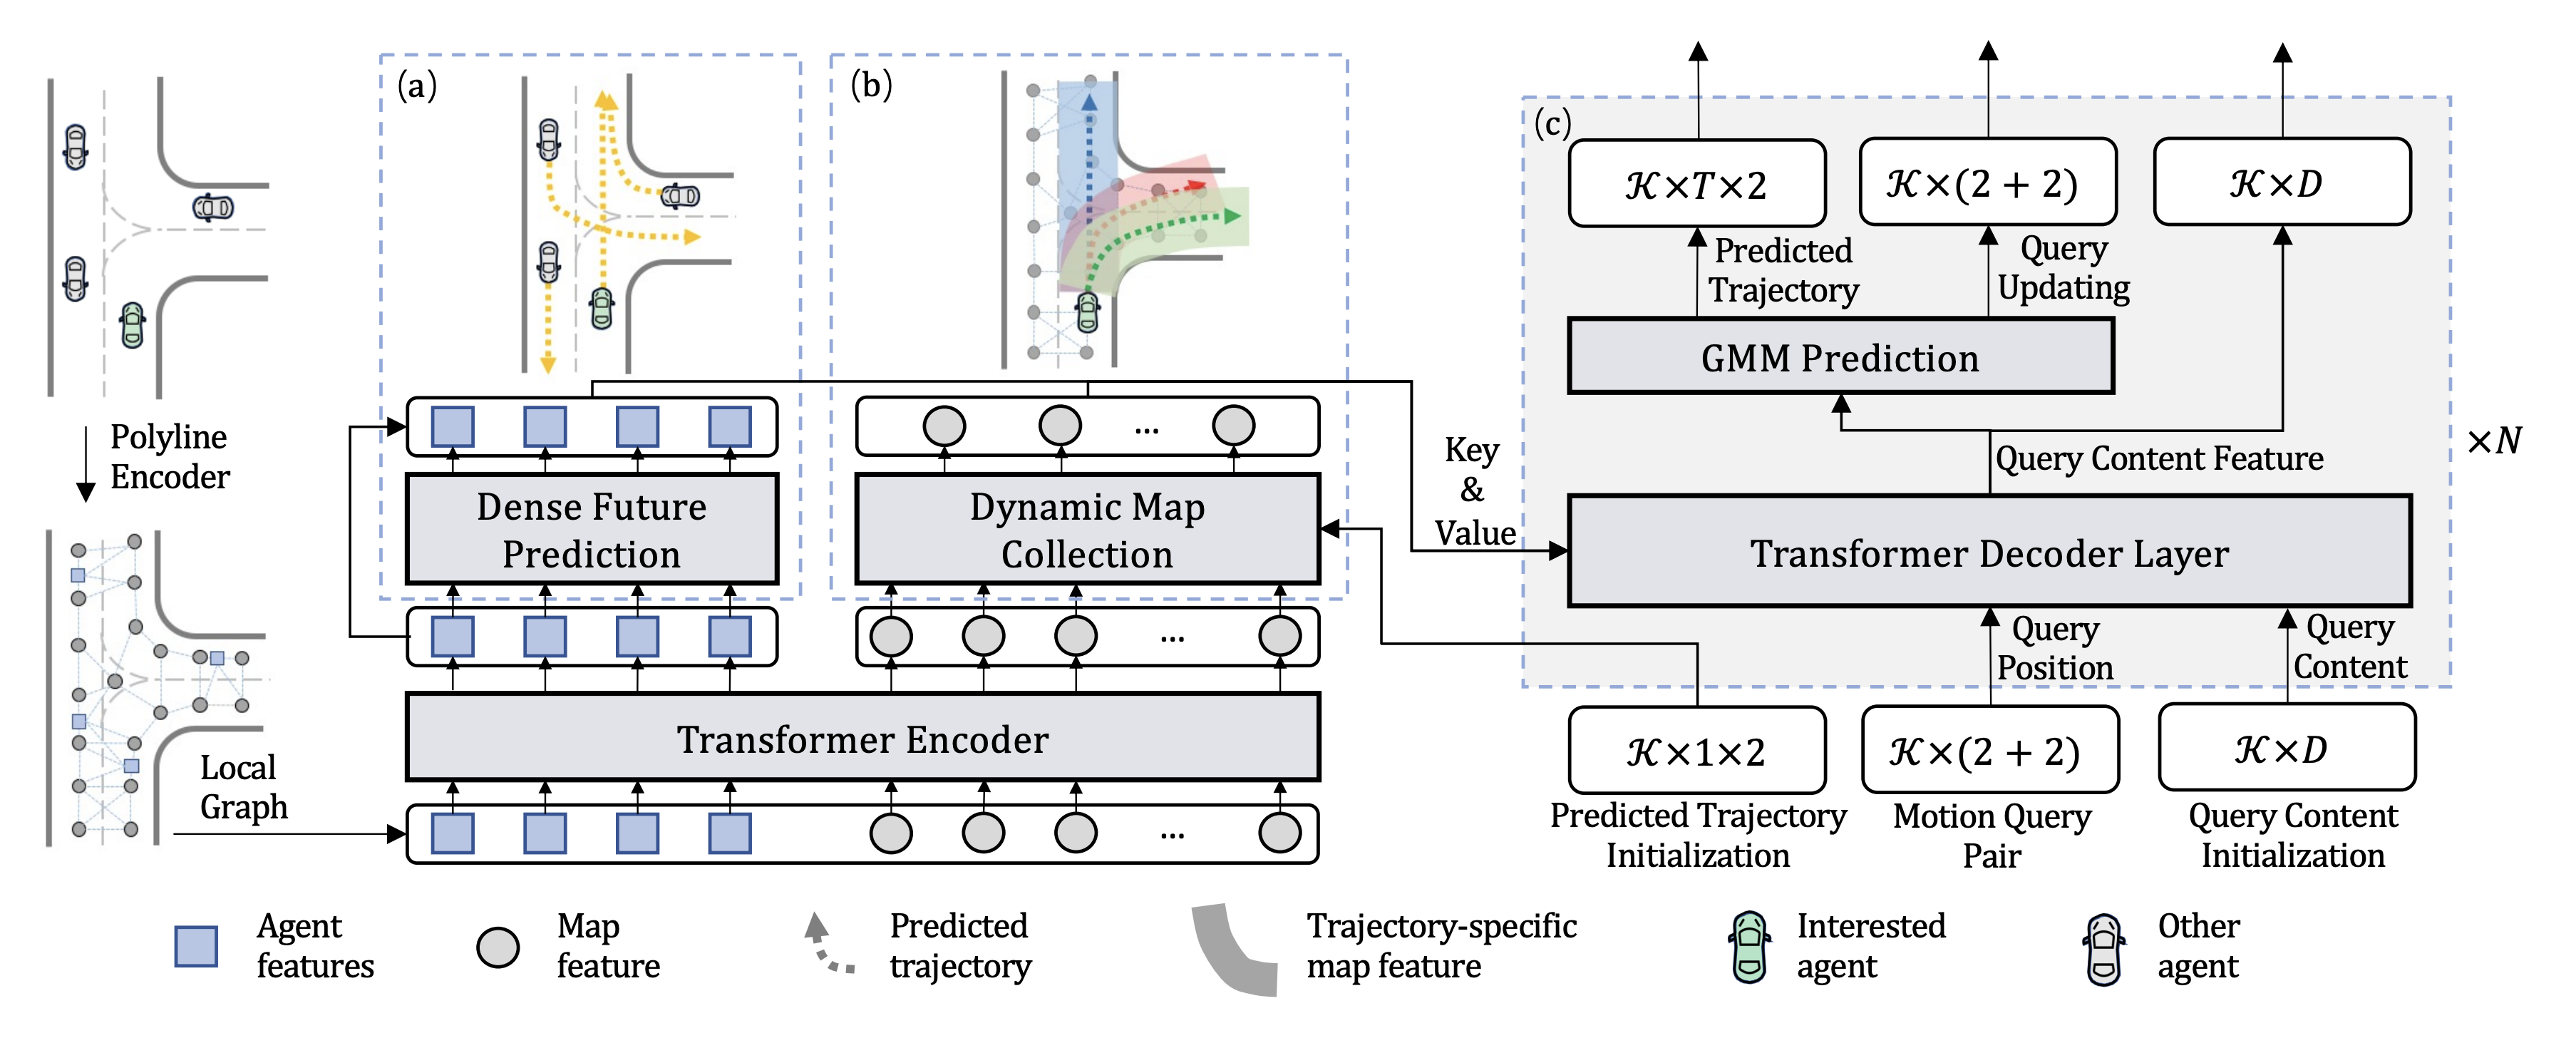
\includegraphics[width=\textwidth]{figures/mtr_overall_architecture_detail.png}
    \caption{A high-level diagram of the MTR architecture, illustrating the flow from vectorized inputs through the scene encoder and motion decoder to the final multimodal trajectory outputs. (Based on Figure 1 from \cite{Shi2022MTR}).}
    \label{fig:mtr_architecture}
\end{figure}

\subsection{Input Encoding}
\label{sec:model_input_encoding}
MTR represents all input data—both from agents and the map—as vectorized polylines, which are sequences of points. This method is more efficient and precise than grid-based representations like bird's-eye-view (BEV) images, as it avoids quantization errors and handles sparse map data well. PointNet-like encoders then process these polylines to generate fixed-size feature vectors for the Transformer model.

\subsubsubsection{Map Encoders}
Map features are represented as a collection of polylines, where each polyline describes a map element like a lane centerline, road boundary, or crosswalk. Each point within a polyline has attributes such as its position (x, y, z) and direction vector. A five-layer MLP processes the points of each map polyline, and a max-pooling operation aggregates this information into a single feature vector ($M_p$) for that polyline. This vector is then projected to a 256-dimensional space to match the agent feature dimensionality.

\subsubsubsection{Agent Encoders}
An agent's historical state is also treated as a polyline. The input for each agent includes its motion history (position, size, heading, velocity) over the last second. To help the model understand the data, several specific features are included:
\begin{itemize}
    \item \textbf{One-hot Category Mask:} This vector identifies the agent's type (e.g., Vehicle, Pedestrian, Cyclist). The model is designed to handle these different agent classes.
    \item \textbf{One-hot Time Embedding:} This feature explicitly encodes the timestep of each point in the history. This is crucial for the Transformer architecture, which does not otherwise have a built-in sense of sequence order.
\end{itemize}
A three-layer MLP processes these point-wise features, and max-pooling creates a 256-dimensional feature vector ($A_p$) for each agent's history.

\subsection{Trajectory Decoding}
\label{sec:model_decoding}
Once the inputs are encoded, the core of the MTR model performs context aggregation and generates predictions.

\subsubsubsection{Transformer Encoder Module}
The feature vectors for all agents ($A_p$) and map polylines ($M_p$) are fed into a Transformer Encoder. This module's job is to contextualize each element by modeling its interactions with its surroundings. To do this efficiently, MTR uses a \textbf{local self-attention} mechanism. Instead of having each element attend to every other element in the scene, it only attends to its $k$ nearest neighbors (e.g., $k=16$). This preserves local structure, reduces computational cost, and improves performance compared to global attention. The output of this stage is a set of context-aware feature vectors for agents ($A_{past}$) and the map ($M$).

\subsubsubsection{Dynamic Map Collection Strategy}
\label{subsec:dynamic_map_collection_strategy}
To ensure that trajectory refinement is guided by the most relevant parts of the map, MTR uses a Dynamic Map Collection strategy within its decoder. For each stage of trajectory prediction, the model identifies the $L$ map polylines (e.g., $L=128$) that are spatially closest to the current trajectory being generated. These selected map features are then used in the decoder's cross-attention mechanism, allowing the model to focus on the immediate local geometry (like lane boundaries for a lane-change maneuver) to make precise, context-aware adjustments.

\begin{figure}[htbp]
    \centering
    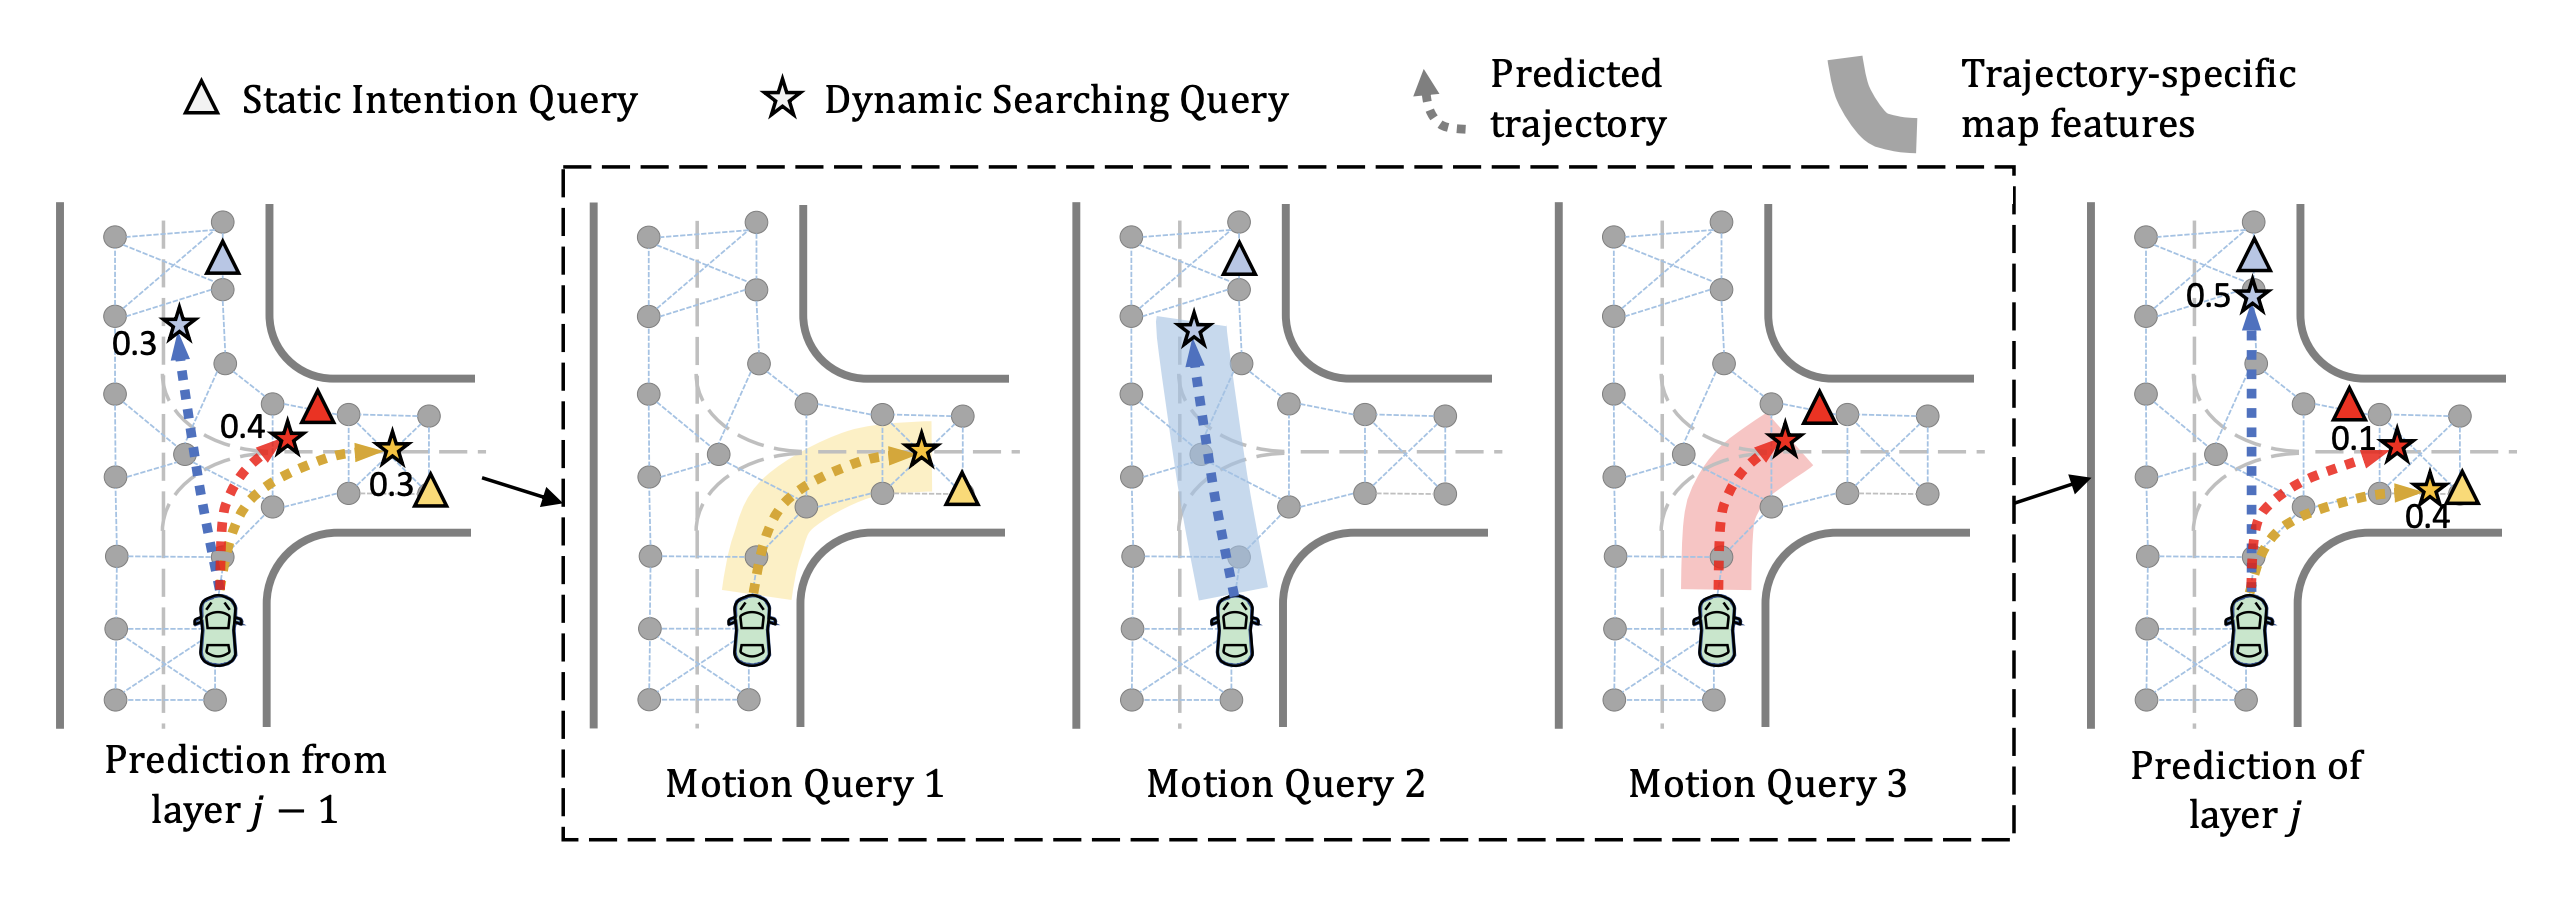
\includegraphics[width=\textwidth]{figures/dynamic_map.png}
    \caption{An illustration of the Dynamic Map Collection strategy. As a trajectory is refined (dashed line), the model selects the L closest map polylines (highlighted) to inform the next prediction step. (Based on Figure 3 from \cite{Shi2022MTR}).}
    \label{fig:dynamic_map}
\end{figure}

\subsubsubsection{Motion Decoder Module (Transformer Decoder Layer)}
The Motion Decoder generates the final trajectory predictions. Its key innovation is the use of \textbf{Motion Query Pairs} to guide this process. Each of the $K$ pairs (e.g., $K=64$) consists of a static query and a dynamic query.

\begin{itemize}
    \item \textbf{Intention-Driven Querying:} The process is driven by two types of queries:
    \begin{itemize}
        \item \textbf{Static Intention Queries ($Q_I$):} These queries act as stable anchors for different motion modes (e.g., turn left, go straight, stop). They are derived from a set of representative ``intention points'', which are pre-calculated by clustering the endpoints of ground-truth trajectories from the training data. Each static query specializes in a specific high-level intention, which helps disentangle the prediction of diverse behaviors and stabilizes training.
        \item \textbf{Dynamic Searching Queries ($Q_S^j$):} These queries perform the fine-grained refinement. At each decoder layer, the dynamic query is updated based on the trajectory predicted by the previous layer. It then probes the scene context (both agent and map features) to gather the specific local details needed to refine that trajectory.
    \end{itemize}
    \item \textbf{Goal-Conditioned Prediction:} The static queries ($Q_I$) enable goal-conditioned prediction. By grounding each of the $K$ prediction modes in a fixed, data-driven intention point, the model generates trajectories that are explicitly conditioned on achieving these latent goals. This synthesizes the strengths of goal-based methods (which are good at capturing multimodality) and direct-regression methods (which are good at generating refined paths).
\end{itemize}

\begin{figure}[htbp]
    \centering
    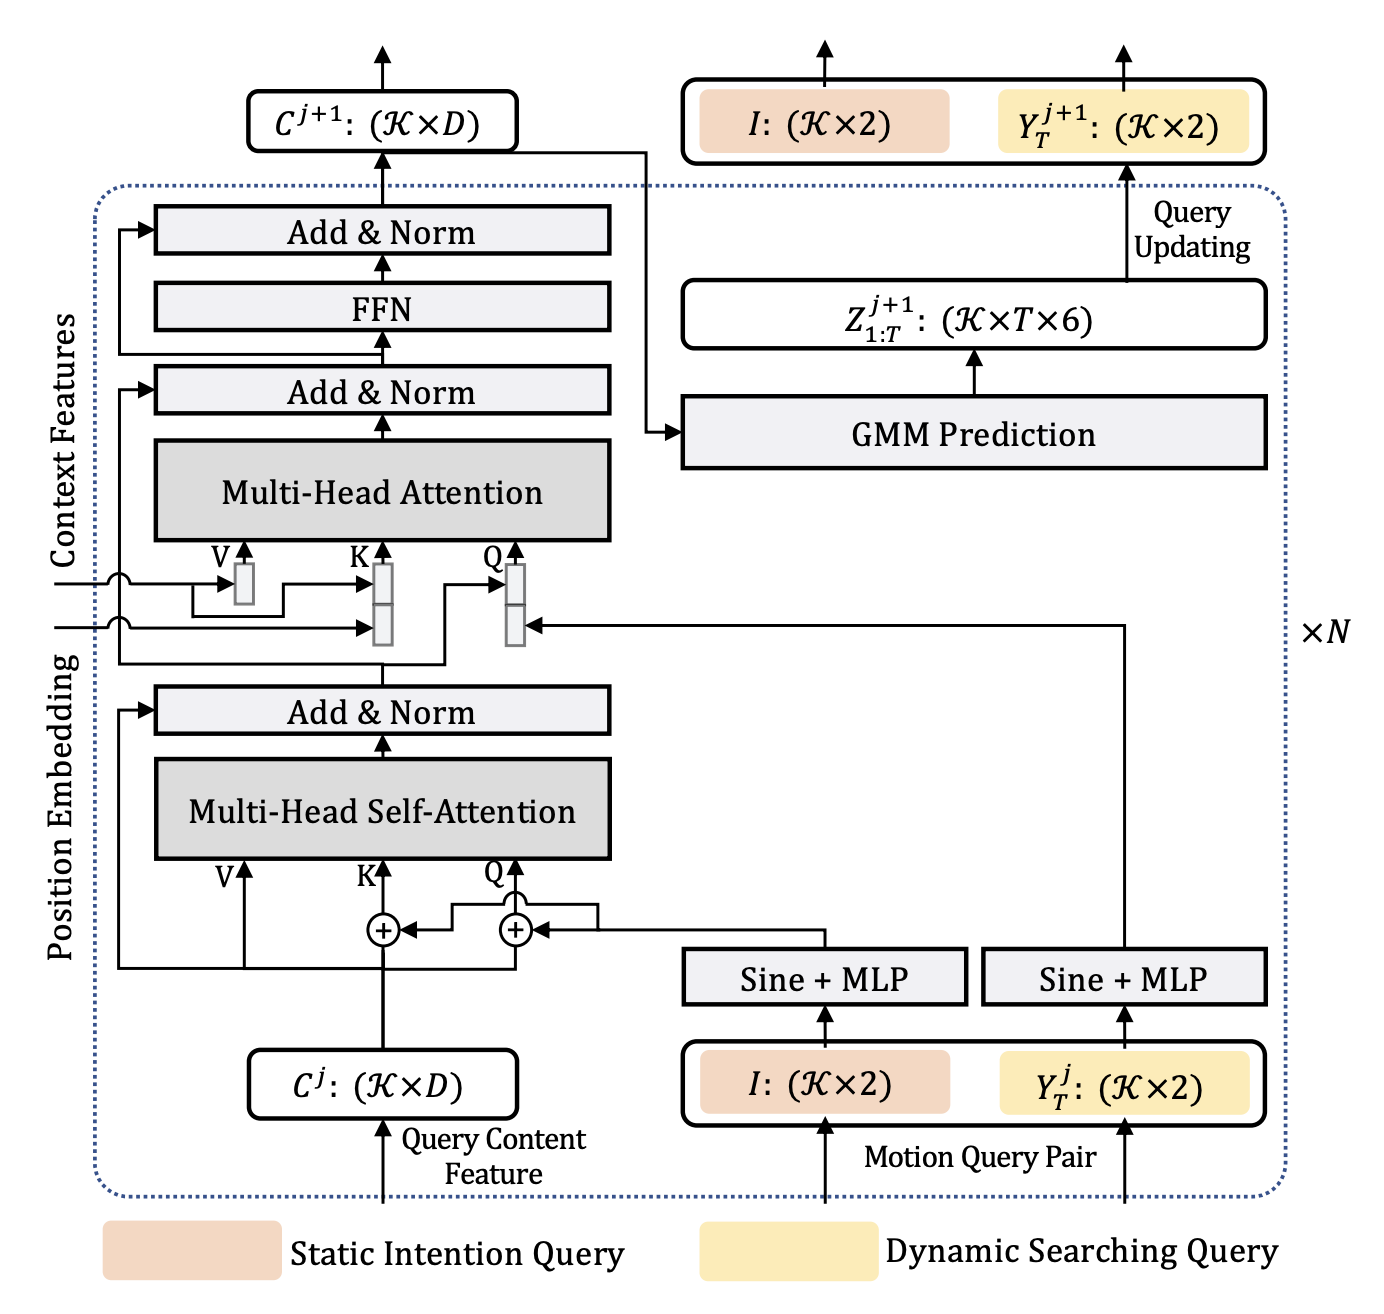
\includegraphics[width=0.6\textwidth]{figures/decoder_layer_detail.png}
    \caption{The architecture of a single Motion Decoder layer, showing how the static intention query ($Q_I$) and dynamic searching query ($Q_S^j$) interact with scene context to refine a trajectory hypothesis. (Based on Figure 2 from \cite{Shi2022MTR}).}
    \label{fig:decoder_layer}
\end{figure}

\subsubsubsection{Probabilistic Multimodal Output Generation}
To represent its multimodal predictions, MTR uses a Gaussian Mixture Model (GMM) as its final output layer. The features from the final decoder layer are passed through an MLP (prediction head) to generate the parameters for $K$ different Gaussian distributions. Each of these $K$ components represents one possible future mode and includes:
\begin{itemize}
    \item A mean trajectory (a sequence of waypoints).
    \item A probability score ($p_k$), which reflects the model's confidence in that specific mode.
\end{itemize}
This probabilistic output provides a rich distribution over plausible futures rather than a single deterministic guess.

\subsubsubsection{Iterative Query Refinement and Training}
The decoder consists of multiple stacked layers (e.g., 6 layers). This stacked structure enables an iterative refinement process. The output trajectory from layer $j-1$ is used to update the dynamic searching query ($Q_S^j$) and to guide the Dynamic Map Collection for layer $j$. Thus, an initial rough trajectory from the first layer is progressively corrected and detailed by subsequent layers, which can focus on more relevant local information.

The model is trained by comparing its $K$ predictions to the single ground-truth trajectory. A loss function guides the model to improve its predictions over time. It essentially encourages the model to assign a high probability ($p_k$) to the predicted trajectory that most closely matches the ground truth, while also moving the waypoints of that trajectory even closer to the actual path. This process can be thought of as a learned form of hypothesis testing: the queries propose $K$ hypotheses, and the training process teaches the model how to evaluate and refine them based on scene context.

\subsection{MTR Input-Output Formulation}
\label{sec:model_mtr_io}

At a high level, the MTR model transforms historical scene data into a set of ranked, probable future paths.

% toDO(luroess): replace figure with improved visualization of input-output visualization
\begin{figure}[htbp]
    \centering
    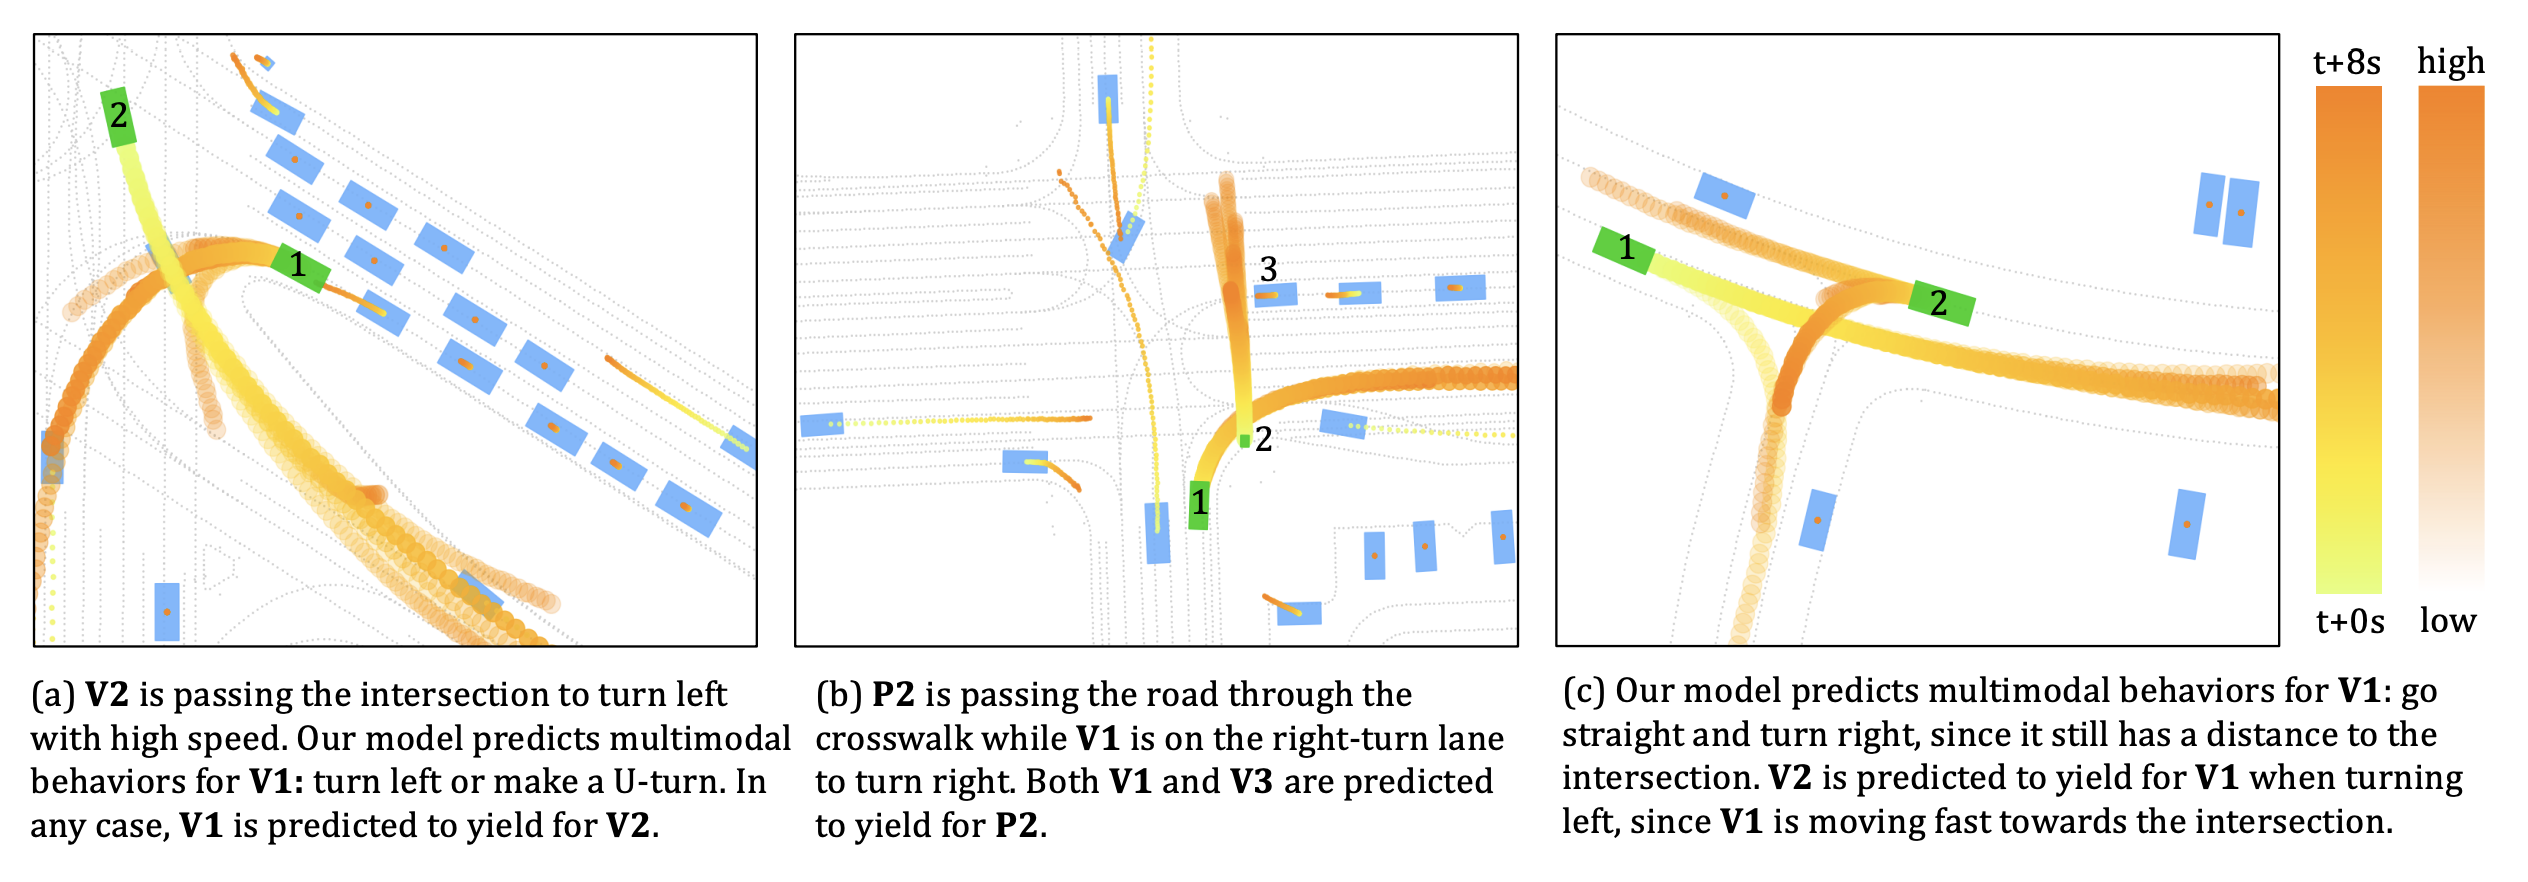
\includegraphics[width=\textwidth]{figures/input_output_viz.png}
    \caption{Qualitative examples of MTR's multimodal predictions in interactive scenarios. The model generates multiple future trajectories (orange paths) for an agent of interest, with agent shwon in green. Other agents are represented by blue boxes. The examples highlight the model's ability to predict socially compliant behaviors, such as yielding to another vehicle (a), a pedestrian (b), or a fast-moving car at an intersubsection (c).}
    \label{fig:input_output_example}
\end{figure}

\begin{itemize}
    \item \textbf{Input Domain:} The minimum necessary input for a single agent's prediction is its historical spatiotemporal data and the features of the surrounding map environment. All input coordinates are normalized into an agent-centric frame, which makes the learning task simpler and invariant to global position and rotation. The framework is designed to process data from large-scale datasets like the Waymo Open Motion Dataset (WOMD). The model can handle various agent types, including vehicles, pedestrians, and cyclists. Within a scene, MTR processes up to 128 context agents, from which a smaller group of up to 8 ``agents of interest'' are designated for prediction, as specified by the WOMD benchmark. The provided documentation focuses on the MTR architecture itself and does not detail specific dataset fusion techniques (e.g., for UniTraj) or agent selection criteria (e.g., based on Kalman difficulty).

    \item \textbf{Output Domain:} The model's exact output is a set of $K$ plausible future trajectories (e.g., $K=64$) for an agent of interest over a future time horizon (e.g., 8 seconds). Each trajectory is defined by a sequence of waypoints and is associated with a probability score ($p_k$) indicating its likelihood. For evaluation against benchmarks that require a smaller number of predictions (e.g., 6), a Non-Maximum Suppression (NMS) algorithm is used to select the most likely and diverse trajectories from the initial set of $K$ proposals.
\end{itemize}

\subsubsection{Illustrative Scenario: Agent at a Crosswalk}
To understand how the components work together, consider a vehicle approaching a crosswalk where a pedestrian is present.
\begin{enumerate}
    \item \textbf{Input and Encoding:} The model takes in the vehicle's past trajectory and the pedestrian's history, along with map polylines for the crosswalk and stop line. These are encoded into feature vectors.
    \item \textbf{Contextualization:} The Transformer Encoder's local attention mechanism allows the vehicle's feature vector to be influenced by the nearby crosswalk and pedestrian features, creating a context-aware representation. An auxiliary task predicts the likely future motion of the pedestrian, further enriching the scene context.
    \item \textbf{Decoding and Prediction:} The Motion Decoder begins its work. Static intention queries propose several plausible high-level actions, such as ``yield before the crosswalk'' and ``proceed through''.
    \begin{itemize}
        \item The ``yield'' hypothesis is refined. Its dynamic query focuses attention on the stop line (via Dynamic Map Collection) and the pedestrian's state.
        \item The ``proceed'' hypothesis is refined similarly.
    \end{itemize}
    \item \textbf{Final Output:} After iterative refinement across the decoder layers, the GMM output will reflect the context. Because the model has taken the pedestrian's presence and future path into account, the probability ($p_k$) associated with the ``yield'' trajectory will be high, while the ``proceed'' trajectory will have a low probability. This demonstrates how MTR generates contextually-aware, multimodal predictions. A visualization of this would show the vehicle's past path, the map features (lanes, crosswalk), and multiple predicted future paths, each with a different color and a displayed probability score.
\end{enumerate}

\subsection{Key Scientific Challenges and Model Variants}

The primary scientific challenge in motion prediction is managing the inherent uncertainty and multimodality of agent behavior in complex, interactive environments. MTR addresses this through its query-based decoder, but different versions of the model optimize for different goals.

\begin{itemize}
    \item \textbf{MTR (Standard):} The baseline model uses $K=64$ queries to generate a rich set of proposals, which are then filtered using NMS. This approach excels at capturing a wide variety of possible behaviors, leading to high performance on metrics like mean Average Precision (mAP).
    \item \textbf{MTR-e2e:} This ``end-to-end'' variant uses only 6 motion queries and no NMS. It is designed for scenarios where a fixed, small number of predictions is required. It uses a different training strategy better suited to the small, adaptive query set.
    \item \textbf{MTR++:} This extension tackles the more complex problem of simultaneous multi-agent prediction. It introduces a shared ``Symmetric Scene Context'' encoder and allows the intention queries of different agents to interact via ``Mutually-Guided Intention Querying''. This enables the model to produce more efficient and scene-compliant joint predictions for all agents at once.
\end{itemize}

These variants show the flexibility of the core MTR architecture in addressing the diverse challenges of motion forecasting.

\subsection{Conclusion}
\label{sec:conclusion}

The Motion Transformer (MTR) architecture addresses the challenge of multimodal motion prediction through its innovative design. Its core strength is the joint optimization of global intention localization and local movement refinement, which is realized through a clear encoder-decoder structure.

The architecture processes vectorized polyline inputs for agent histories and map features with PointNet-like encoders. A Transformer encoder then uses local self-attention to build a rich, contextualized scene understanding. The subsequent Motion Decoder uses its key components to generate predictions. Static intention queries ($Q_I$) provide stable, mode-specific anchors based on data-driven intention points. Dynamic searching queries ($Q_S^j$) then perform precise, context-aware refinement of these intentions. This refinement is guided by prior predictions and a dynamic map collection strategy ($\alpha(M)$). The stacked decoder layers iteratively improve the trajectories, and a final prediction head produces a probabilistic set of future paths using a Gaussian Mixture Model (GMM).

Model variants show the architecture's flexibility. MTR-e2e adapts the model for end-to-end prediction with a fixed number of outputs, while the MTR++ extension enables efficient and interactive multi-agent prediction. These architectural choices allow MTR to generate accurate, diverse, and scene-compliant trajectory forecasts. The principles of query-based prediction, iterative refinement, and adaptive context utilization are valuable paradigms for future work in autonomous navigation.
\subsection{LMFormer}
\label{ssec:lmformer}

\paragraph{Polyline Representations} motion vectors: $\mathcal{T}_{out}^{a,m} = [(V_1^{a,m}, S_1^{a,m}), (V_2^{a,m}, S_2^{a,m}), ..., (V_{T'}^{a,m}, S_{T'}^{a,m})]$, where $V_t^{a,m} = [P_{t-1}^{a,m}, P_t^{a,m}]$ represents the motion vector for agent $a$, mode $m$, and time step $t$, with associated variance $S_t^{a,m}$.


\subsubsection{Recurrent Temporal Decoding}
Following successful applications in CASPFormer~\cite{caspformerYadav2024} and QCNet~\cite{Zhou2023QueryCentric}, LMFormer incorporates recurrent temporal decoding ($\times T_{out}$) in cross-attention modules. Each recurrent loop updates both the query position and the query itself, enabling progressive refinement of trajectory predictions.

The decoder employs three specialized cross-attention mechanisms:
\begin{itemize}
    \item \textbf{Mode2Temporal Cross Attention:} Aggregates temporal information from Agent Encodings (keys/values) to mode queries
    \item \textbf{Mode2Agent Cross Attention:} Enables each mode of an agent to attend to corresponding modes of other agents, modeling future social interactions
    \item \textbf{Mode2Lane Cross Attention:} Incorporates static context information from Lane Encodings into mode queries
\end{itemize}
% 6. Empirical Evaluation and Results 
\section{Experimental Design and Performance Evaluation}
\label{ch:experimental_design_and_results}

This chapter details the framework for training and evaluating the trajectory prediction model. It outlines the experimental setup, the learning objectives, and the metrics used for assessment, followed by a quantitative and qualitative analysis of the model's performance.

% 5. subsection: Training and Evaluation Paradigm 
\subsection{Training and Evaluation Paradigm}
\label{sec:training_and_evaluation_paradigm}

The training and evaluation environment uses a robust and reproducible setup. This subsection details the computational environment, configuration management, and the data processing pipeline.

\subsubsubsection{Training Environment and Configuration}
\label{sec:exp_training_env_merged}
% Specification of the computational setup (PyTorch Lightning, WandB for experiment tracking and logging) and critical hyperparameters. 
% Discussion of the rationale behind the selected configurations. 

The entire suite for training, evaluation, and logging is managed through PyTorch Lightning, with experiment tracking and visualization handled by Weights \& Biases (WandB). This setup facilitates managed logging, checkpointing, and distributed training strategies.

All configurations and hyperparameters are managed by Pydantic. This enables a ``Config-as-Factory'' pattern, which simplifies the process of swapping different models, datasets, or loss functions. While the environment is robustly configured, the provided documentation does not detail specific hyperparameters such as batch size or learning rate.

\subsubsubsection{Data Handling and Processing}
\label{sec:data_handling_merged}

For high-throughput data ingestion, the data loading pipeline uses HDF5. The framework enhances processing efficiency by randomly partitioning the full sample index into 32 shards and assigning one shard to each DataLoader worker, which ensures balanced and parallel prefetching.

% - How iterative improvements are achieved during training (e.g. loss on intermediate decoder layers for MTR ). 
The training data undergoes a detailed processing pipeline before being fed to the model:
\begin{itemize}
    \item \textbf{Agent Selection:} First, the pipeline selects agents—vehicles, pedestrians, or cyclists—based on their movement distance and visibility within scenarios.
    \item \textbf{Scenario Classification:} Scenarios receive a difficulty classification (Easy, Medium, Hard) derived from a Kalman filter analysis.
    \item \textbf{Coordinate Normalization:} The system then normalizes all coordinate data into an agent-centric frame using the rotation matrix $R_{z}(-\theta_{c})$.
    \item \textbf{Tensor Assembly:} Finally, it assembles agent and map features into padded and masked tensors, specifically $\mathbb{R}^{N_{max}\times T_{p}\times F_{ap}}$ for dynamic agent data and $\mathbb{R}^{K\times L\times F_{map}}$ for static map data, preparing them for model ingestion.
\end{itemize}

\subsection{Optimization Strategy and Learning Objective}
\label{sec:exp_optimization_merged}

The MTR model was trained from scratch without the use of a pre-trained model. A significant portion of the implementation involved adapting the model to the UniTraj framework's data parsing and configuration systems.
% - The overall objective the model is trained to optimize. 
The primary learning objective is to train the model to accurately forecast multimodal trajectories.

% Detailed specification of the loss function(s) employed for MTR training, including components for trajectory regression and mode probability classification. 
% - Specific loss components and their roles. 
% - e.g., For MTR: Gaussian Regression Loss (NLL) and auxiliary L1 regression loss. 
% - Any specific strategies like hard assignment in MTR. 
% Discussion of how this objective function guides the model to learn multimodal distributions (e.g., relationship to Brier-FDE if incorporated). 
The UniTraj framework unifies loss functions for different models, and the overall training objective is to minimize these functions to improve prediction accuracy. The training process specifically seeks to decrease metrics like the minimum Final Displacement Error (FDE). A key component of the objective is the Brier Final Displacement Error, which assesses both the accuracy of the trajectory's final point and the model's confidence in its prediction. This objective guides the model to learn multimodal distributions. However, the exact mathematical formulation of the loss function used for this training run is not specified in the source material. 
% e.g., Adam optimizer with specified learning rate and scheduling. 
% - Optimizer used, learning rate, batch size, epochs etc. 
Similarly, the specific optimization algorithm, such as Adam or SGD, and its associated parameters like learning rate and scheduling, are not mentioned.

\subsection{Evaluation Metrics}
\label{sec:exp_metrics_merged}

The model's performance assessment relies on a set of standard industry metrics. The mathematical definitions for these metrics are as follows:
\begin{itemize}
    \item \textbf{Average Displacement Error (ADE):} The mean L2 distance between the predicted trajectory and the ground truth across all time steps, defined as $ADE=\mathbb{E}_{t}[||\hat{y}_{t}-y_{t}||_{2}]$.
    \item \textbf{Final Displacement Error (FDE):} The L2 distance between the final predicted position and the ground truth final position, given by $FDE=||\hat{y}_{T}-y_{T}||_{2}$.
    \item \textbf{Miss Rate (MR):} The fraction of predictions where the FDE for the most likely trajectory exceeds a distance threshold $d_{thresh}$ (e.g., 2.0 m). The formula is $MR=\mathbb{E}_{k}[\mathbb{I}\{||\hat{y}_{T}^{(k)}-y_{T}||_{2}>d_{thresh}\}]$.
    \item \textbf{Brier Final Displacement Error (BrierFDE):} A metric that scores both trajectory accuracy and its assigned probability, defined as $BrierFDE=\mathbb{E}_{k}[p_{k}\cdot||\hat{y}_{T}^{(k)}-y_{T}||_{2}^{2}]$.
\end{itemize}

\subsection{Performance Analysis}
\label{sec:performance_analysis_merged}
This subsection evaluates the trained MTR model's performance through quantitative metrics and qualitative review. The analysis confirms the model's learning effectiveness and its ability to generate accurate and probable trajectory forecasts.

\subsubsubsection{Quantitative Performance Analysis}
\label{sec:results_quantitative_merged}
% Presentation and statistical analysis of validation metrics (brier-minFDE, minFDE, minADE, Miss Rate). 
% Add actual results, tables, figures. 
% Comparison against reported benchmarks (e.g., UniTraj paper results ), with careful consideration of comparability. 

The quantitative analysis of the MTR model's performance is based on metrics recorded during training and validation. The training process shows a clear reduction in loss values, indicating the model is learning from the data. The plots in Figure \ref{fig:training_metrics_grid_merged} exhibit a characteristic learning curve: a steep reduction in error during initial training, which then gradually plateaus. This trend indicates convergence.

% toDO(luroess): Split graphs for better visualization?
\begin{figure}[htbp]
    \centering
    \begin{subfigure}[b]{0.48\textwidth}
        \centering
        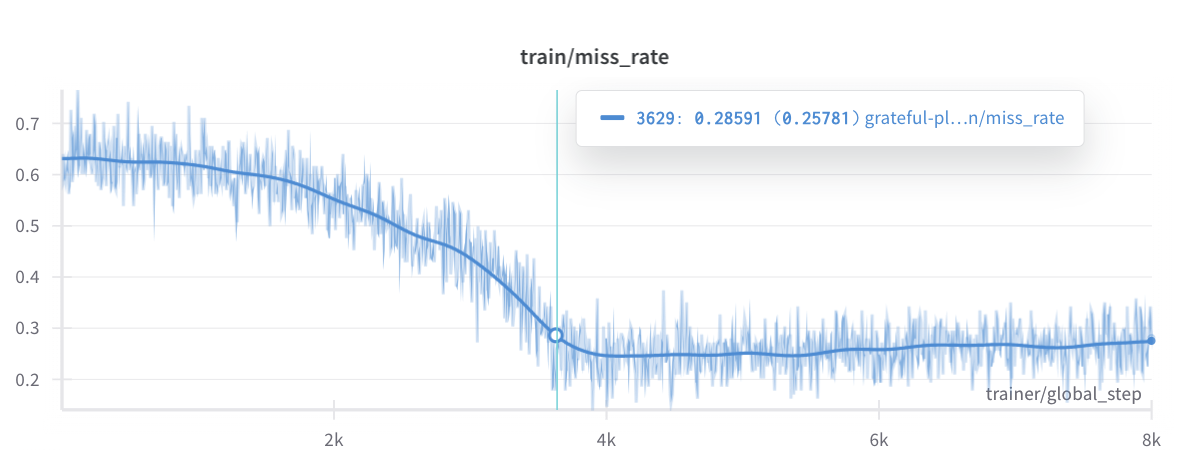
\includegraphics[clip, width=\textwidth]{figures/train_miss_rate.png}
        \caption{train/miss\_rate}
    \end{subfigure}
    \hfill
    \begin{subfigure}[b]{0.48\textwidth}
        \centering
        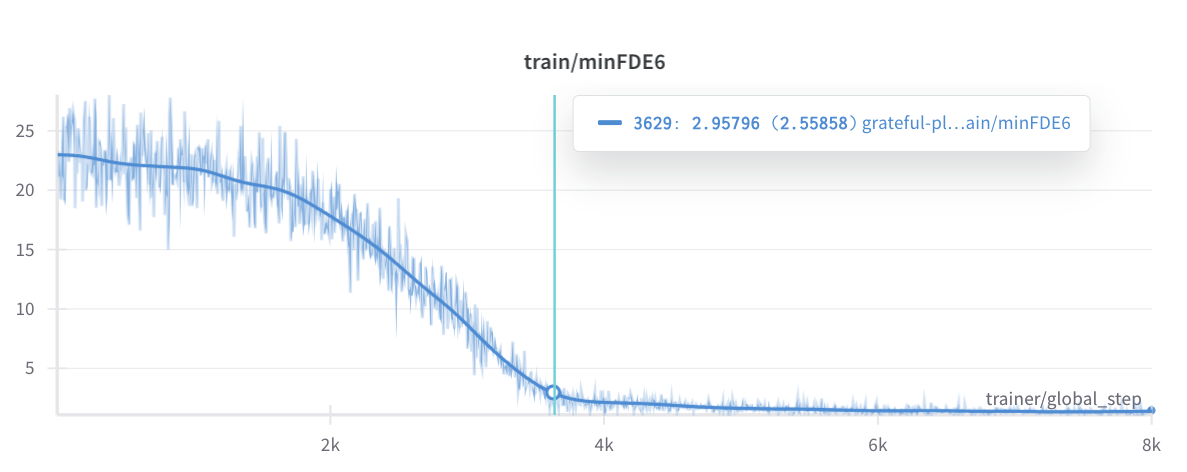
\includegraphics[clip, width=\textwidth]{figures/train_min_fde6.png}
        \caption{train/minFDE6}
    \end{subfigure}
    \vfill
    \begin{subfigure}[b]{0.48\textwidth}
        \centering
        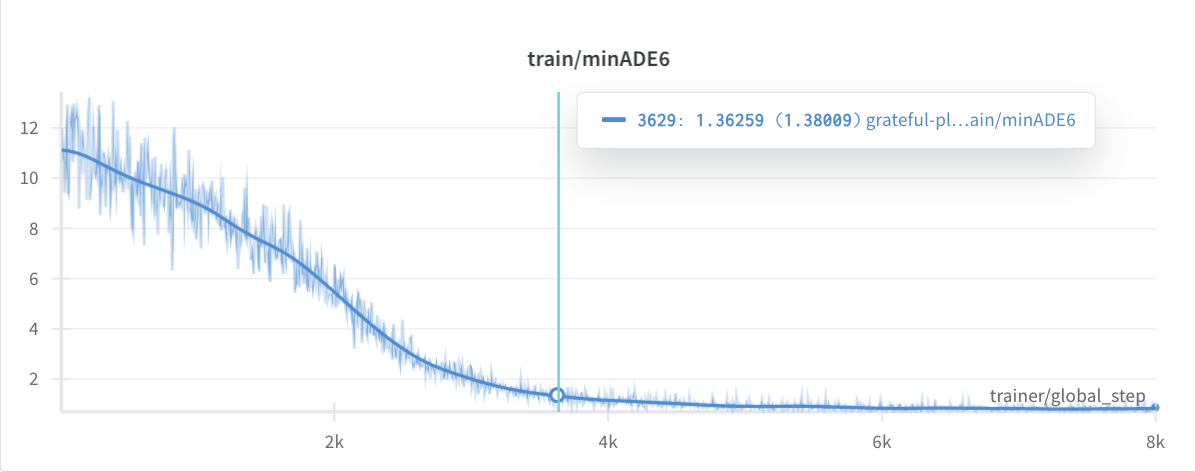
\includegraphics[clip, width=\textwidth]{figures/train_min_ade6.png}
        \caption{train/minADE6}
    \end{subfigure}
    \hfill
    \begin{subfigure}[b]{0.48\textwidth}
        \centering
        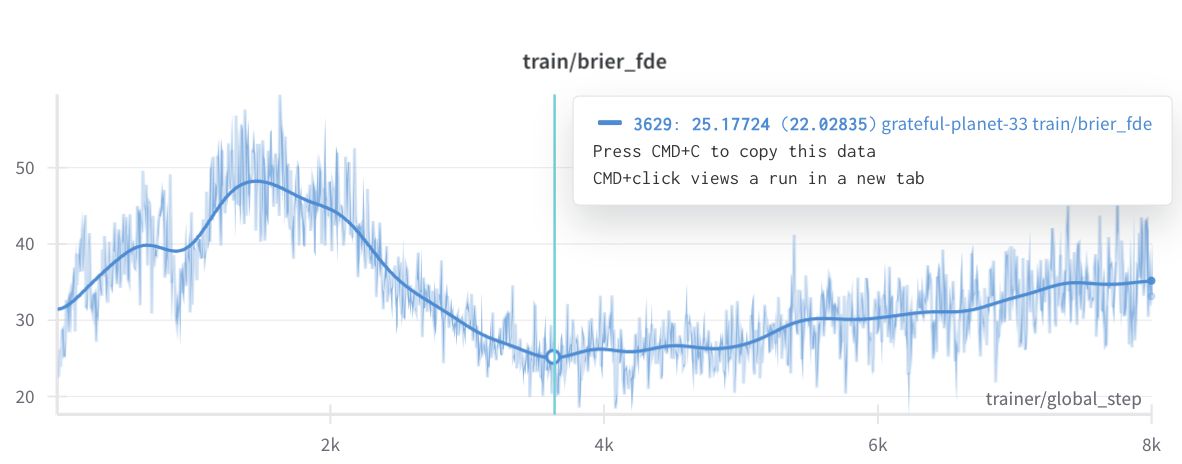
\includegraphics[clip, width=\textwidth]{figures/train_brier_fde.png}
        \caption{train/brier\_fde}
    \end{subfigure}
    \caption{A grid of performance metrics on the training set. The plots show a consistent decrease in error for miss rate, brier FDE, minFDE6, and minADE6 over approximately 6,000 training step of batches, which indicates successful learning. }
    \label{fig:training_metrics_grid_merged}
\end{figure}

Final validation metrics, taken at step 31,295 (6,259 batches), are presented in Table \ref{tab:validation_results}.  On the validation set, the trained MTR model achieved a brier-minFDE of 1.98, a minFDE of 1.6655, a minADE of 0.86294, and a Miss Rate of 0.30141.  These results are comparable to baseline values from existing literature.  The consistent decrease in error seen in Figure \ref{fig:validation_metrics_merged} demonstrates that the model generalizes well to unseen data.  Notably, the Brier-FDE of 1.98 shows a slight improvement over the 2.08 value reported in the MTR paper's appendix, highlighting the effectiveness of this training implementation. 

\begin{table}[htbp]
    \centering
    \caption{Final Validation Metrics at Step 31,295}
    \label{tab:validation_results}
    \begin{tabular}{@{}lcc@{}}
        \toprule
        \textbf{Metric} & \textbf{Value} & \textbf{Benchmark (MTR Paper)} \\
        \midrule
        brier-minFDE & 1.98  & 2.08  \\
        minFDE & 1.6655  & - \\
        minADE & 0.86294  & - \\
        Miss Rate & 0.30141  & - \\
        \bottomrule
    \end{tabular}
\end{table}

% toDO(luroess): Split graphs for better vizualization?
\begin{figure}[htbp]
    \centering
    \begin{subfigure}[b]{0.48\textwidth}
        \centering
        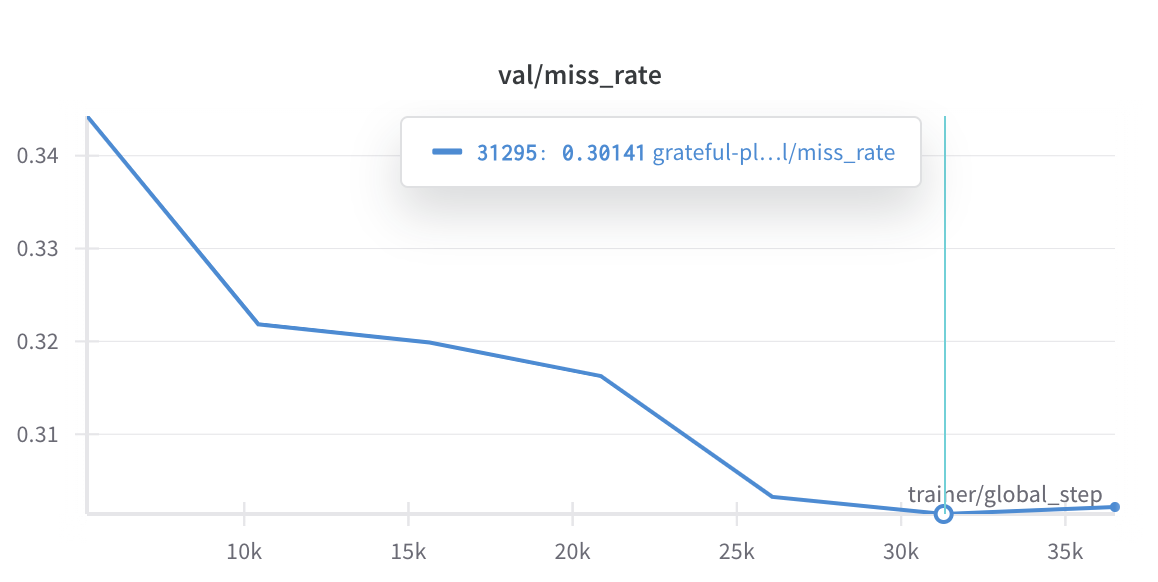
\includegraphics[clip, width=\textwidth]{figures/val_miss_rate.png}
        \caption{val/miss\_rate: 0.30141}
    \end{subfigure}
    \hfill
    \begin{subfigure}[b]{0.48\textwidth}
        \centering
        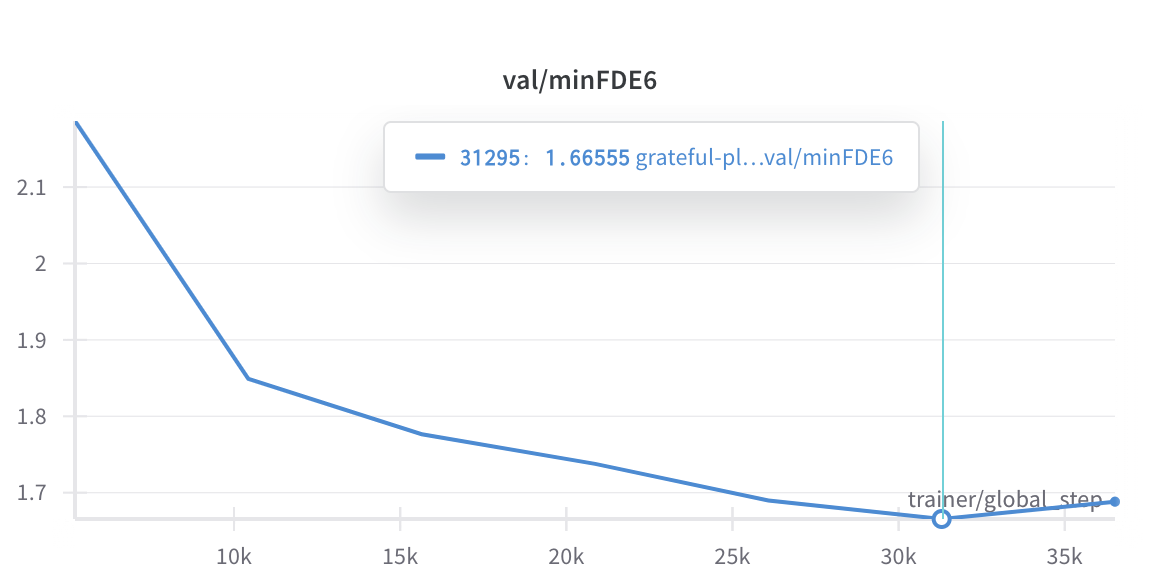
\includegraphics[clip, width=\textwidth]{figures/val_min_fde6.png}
        \caption{val/minFDE6: 1.6655}
    \end{subfigure}
    \vfill
    \begin{subfigure}[b]{0.48\textwidth}
        \centering
        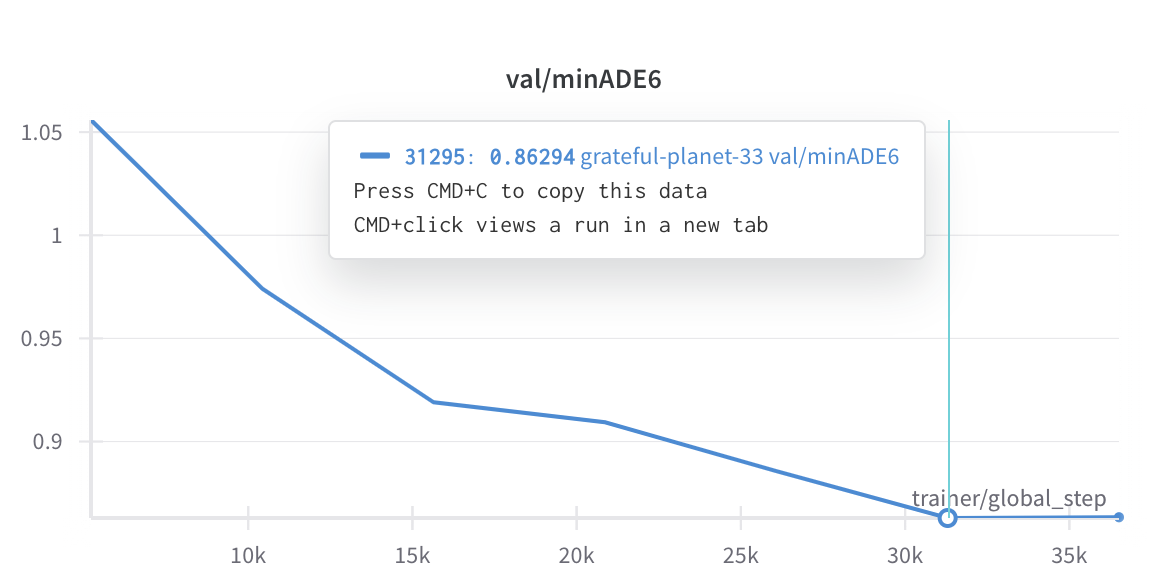
\includegraphics[clip, width=\textwidth]{figures/val_min_ade6.png}
        \caption{val/minADE6: 0.86294}
    \end{subfigure}
    \hfill
    \begin{subfigure}[b]{0.48\textwidth}
        \centering
        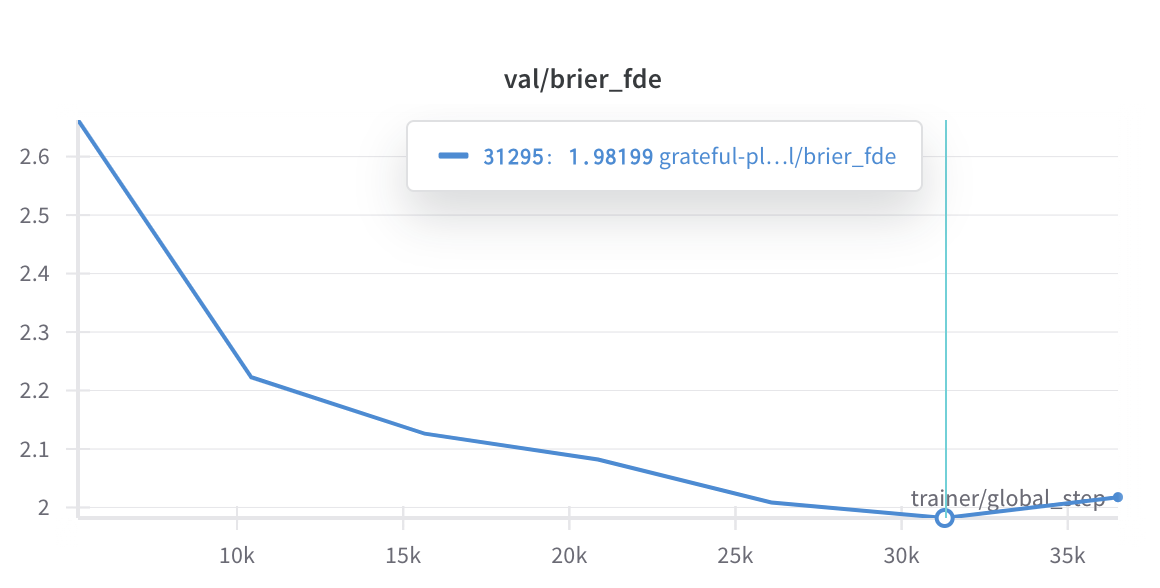
\includegraphics[clip, width=\textwidth]{figures/val_brier_fde.png}
        \caption{val/brier\_fde: 1.98199}
    \end{subfigure}
    \caption{Performance metrics on the validation set during MTR training. The plots show a consistent decrease in error for miss rate, FDE, ADE, and Brier-FDE as training progresses. }
    \label{fig:validation_metrics_merged}
\end{figure}

\subsubsubsection{Qualitative Analysis and Sample Case Illustration}
\label{sec:results_qualitative_merged}
% Detailed deconstruction of prediction examples (cf. presentation slides 10, 15 ), identifying ego agent, other agents, ground truth trajectories, and probabilistic forecasted paths. 
% Analysis of the influence of map topology (lanes, crosswalks) on predicted modalities. 
% Examination of model predictions in critical scenarios (e.g., agent behavior at intersubsections or pedestrian crossings), linking observed outputs to specific input features and model mechanisms. 
The qualitative analysis involves a detailed deconstruction of prediction examples. This process identifies the ego agent, other agents, ground truth trajectories, and the probabilistic forecasted paths generated by the model. The analysis also examines the influence of map topology, such as lanes and crosswalks, on the predicted modalities. Furthermore, it includes the examination of model predictions in critical scenarios, like agent behavior at intersubsections or pedestrian crossings, to link observed outputs to specific input features and model mechanisms.

Figure \ref{fig:mtr_prediction_merged} serves as a sample case, showing a multimodal prediction for a right-turn scenario. The model generates multiple future trajectories and assigns a probability to each. The green line represents the ground truth future path, while the colored lines show the model's predictions, with one having a much higher probability (p=0.36) than another (p=0.02).

% toDO(luroess): Generate new visualization for MTR prediction, this looks awful 
\begin{figure}[htbp]
    \centering
    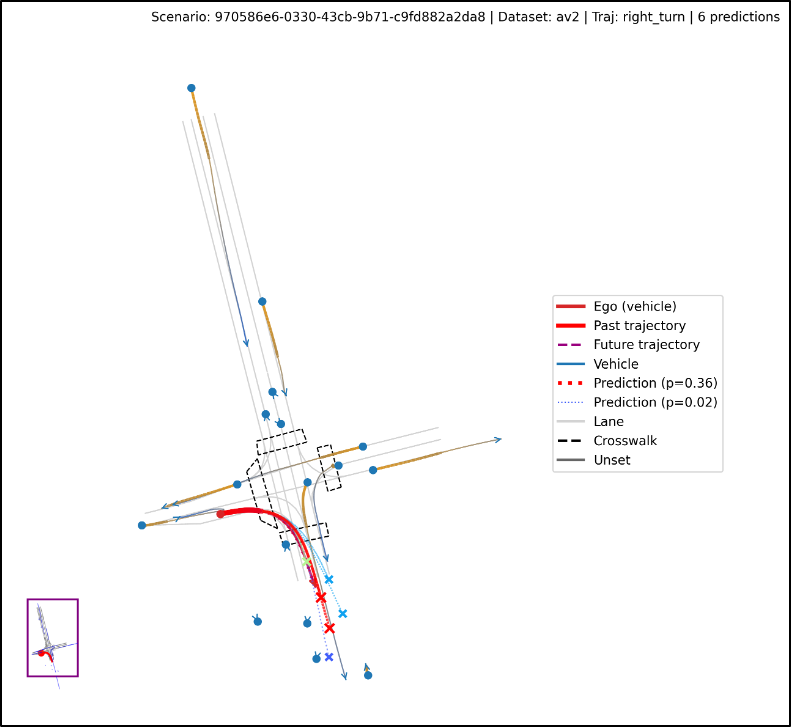
\includegraphics[width=0.8\textwidth]{figures/input_output_viz_ugly.png}
    \caption{A multimodal prediction from the MTR model for a right-turn scenario. The green line is the ground truth, and the colored lines are predictions with different probabilities.}
    \label{fig:mtr_prediction_merged}
\end{figure}
% 8. Conclusion and Discussion
\section{Conclusion and Discussion}
\label{sec:conclusion}
% - The research's most significant outcomes were summarized.
% - The project was impacted by a scope reduction, such as focusing on "Very-Smol-Single-Agent-Motion-Forecasting".
% - Data deficiencies, like the absence of BBOX from AV2 and restriction to vehicle-only agent types, had consequences.
% - An assessment of the UniTraj Framework covered reported issues in coding standards, documentation, and framework (PyTorch Lightning, WandB) utilization.
% - Challenges with the UniTraj Framework related to data integrity (original splits), file management, logging practices, and software design patterns were discussed.
% - An overview of applied refactoring efforts and mitigation strategies for the UniTraj Framework was provided.
% - The fulfillment of initial objectives was addressed.
This research successfully demonstrated the viability of the query-centric paradigm for trajectory prediction in autonomous driving, achieving competitive performance metrics with our Smol-LMFormer implementation. The most significant outcomes include the successful integration of the UniTraj framework~\cite{unitrajFeng2024} with modern deep learning infrastructure, achieving a brier-minFDE of 1.98 compared to the MTR benchmark of 2.08, and establishing a robust experimental pipeline using PyTorch Lightning~\cite{falcon2019pytorch} and Weights \& Biases for comprehensive experiment tracking. However, the project scope was significantly reduced from the initial multi-agent joint prediction objectives to focus on "Very-Smol-Single-Agent-Motion-Forecasting" due to computational constraints and framework limitations. Data deficiencies substantially impacted model development, particularly the absence of bounding box information from Argoverse2~\cite{av2Wilson2023} and the restriction to vehicle-only agent types, limiting our ability to evaluate pedestrian and cyclist prediction capabilities that are crucial for comprehensive autonomous driving systems. Our assessment of the UniTraj framework revealed critical issues in coding standards, inadequate documentation, and suboptimal utilization of modern ML frameworks like PyTorch Lightning and WandB, aligning with known software quality challenges in autonomous driving research~\cite{metadriveLi2022}. Additional challenges included data integrity issues with original dataset splits, poor file management practices, insufficient logging mechanisms, and violation of established software design patterns, necessitating extensive refactoring efforts that consumed significant development time. Despite these challenges, our mitigation strategies successfully established a reproducible training pipeline and demonstrated the effectiveness of query-centric representations~\cite{qcnetZhou2023} for single-agent trajectory forecasting, laying the foundation for future multi-agent extensions.

\subsection{Reflection on Initial Objectives}
\label{sec:conclusion_objectives}

The initial aim of this seminar work was to implement a minimal, simplified model for trajectory prediction in autonomous driving. However, the complexity of existing algorithms made this goal impractical. As detailed in Chapter~\ref{ch:model_architecture}, the intricate data pipelines, geometric invariance requirements, and interdependent components of frameworks like UniTraj prevented meaningful simplification without losing essential functionality.

This complexity necessitated the extended analysis presented throughout this report, particularly the comparative study in Chapter~\ref{sec:background}examining agent-centric versus query-centric paradigms. While the original implementation goal proved unattainable, the work achieved a thorough understanding of these fundamental approaches. The investigation clarified how query-centric methods enable permutation and $\mathrm{SE}(2)$-equivariance while supporting streaming inference and joint prediction, contrasting with the limitations of agent-centric frameworks bound to privileged reference frames.

Engaging with state-of-the-art transformer architectures deepened our understanding of attention mechanisms for encoding spatial and temporal relationships in trajectory forecasting. The experimental work described in Chapter~\ref{ch:experimental_design_and_results} demonstrated practical application of these concepts, despite scope limitations to single-agent prediction.

Although the minimal implementation remained beyond reach, the seminar work succeeded in building conceptual foundations and critical perspective on current research directions. The experience highlighted the importance of clear abstractions and robust data handling while exposing the challenges inherent in adapting complex frameworks for educational purposes.


% Include appendix
% Appendix
\appendix
\section{Appendix}

\subsection{Notation and Symbol Reference}
\label{app:notation}

This section provides a comprehensive reference for all symbols and conventions used throughout this work, following UniTraj framework standards~\cite{unitrajFeng2024} and the \textsc{DatasetItem} type definitions. The following tables have been created using~\cite{copilotSonnet}, given the type and shape definitions in \href{https://github.com/JanDuchscherer104/UniTraj/blob/main/unitraj/datasets/types.py}{unitraj/datasets/types.py}.

\begin{table}[H]
\caption{Temporal dimension symbols and definitions}
\centering
\begin{tabular}{p{3cm}p{10cm}}
\toprule
\textbf{Symbol} & \textbf{Definition} \\
\midrule
\(T_p, T_{\text{in}}\) & Number of past timesteps (historical context) \\
\(T_f, T_{\text{out}}\) & Number of future timesteps (prediction horizon) \\
\(T\) & Total trajectory length: \(T = T_p + T_f\) \\
\(\Delta t\) & Temporal sampling interval (i.e.\ 0.1s for 10Hz data) \\
\bottomrule
\end{tabular}
\end{table}

\begin{table}[H]
\caption{Spatial and agent dimension symbols}
\label{tab:shape_symbols}
\centering
\begin{tabular}{p{3cm}p{10cm}}
\toprule
\textbf{Symbol} & \textbf{Definition} \\
\midrule
\(N_{\max}\) & Maximum number of agents in scene (i.e.\ 64) \\
\(N, N_A\) & Actual number of agents in a specific scenario \\
\(N_c\) & Number of center agents, \(N_c = N \) in \cite{lmformerYadav2025}. \\
\(K_{\max}\) & Maximum number of map polylines (i.e.\ 256) \\
\(K\) & Actual number of map polylines in a specific scenario \\
\(L\) & Number of points per map polyline (i.e.\ 20) \\
\( N_L\) & Number of lane segments in \( \boldsymbol{X}_s, N_L=K \cdot L \) \\
\(F_{ap}\) & Agent feature dimension (i.e.\ 39) \\
\(F_{af}\) & Agent future state dimension (4: \(x, y, v_x, v_y\)) \\
\(F_{map}\) & Map feature dimension (i.e.\ 29) \\
\(D\) & Hidden dimension of encodings or latent representations. \\
\bottomrule
\end{tabular}
\end{table}

\begin{table}[H]
\caption{Primary data tensors and their shapes}
\label{tab:data_tensors}
\centering
\begin{tabular}{p{4cm}p{9cm}}
\toprule
\textbf{Tensor} & \textbf{Shape and Description} \\
\midrule
\(\boldsymbol{X}_d\) & \([N_{\max}, T_p, F_{ap}]\) Agent trajectory features \\
\(\boldsymbol{M}_d\) & \([N_{\max}, T_p]\) Agent trajectory validity mask \\
\(\boldsymbol{X}_{d,pos}\) & \([N_{\max}, T_p, 3]\) Agent positions \((x, y, z)\) \\
\(\boldsymbol{X}_{d,last}\) & \([N_{\max}, 3]\) Last observed agent positions \\
\(\tilde{\boldsymbol{X}}_d\) & \([N_{\max}, T_f, F_{af}]\) Agent future states \\
\(\tilde{\boldsymbol{M}}_d\) & \([N_{\max}, T_f]\) Agent future validity mask \\
\(\boldsymbol{y}_c\) & \([T_f, F_{af}]\) Center agent ground truth trajectory \\
\(\boldsymbol{M}_c\) & \([T_f]\) Center agent ground truth validity mask \\
\(\boldsymbol{X}_s\) & \([K_{\max}, L, F_{map}]\) Map polyline features \\
\(\boldsymbol{M}_s\) & \([K_{\max}, L]\) Map polyline validity mask \\
\(\boldsymbol{C}_s\) & \([K_{\max}, 3]\) Map polyline centers \\
\bottomrule
\end{tabular}
\end{table}

Here, \( \tilde{\bullet}_{\circ} \) denotes tensors, expressing future states, while \(\bullet_{\circ}\) denotes tensors for historical or static context. \( \bullet_{d} \) denotes all tensors, representing \emph{dynamic} agents, while \(\bullet_{s}\) denotes tensors for \emph{static} map elements. The center agent, whose trajectory is the target for prediction, is denoted by the subscript \(c\).

\begin{table}[H]
\caption{Agent feature components ($F_{ap} = 39$)}
\centering
\begin{tabular}{p{3cm}p{3cm}p{7cm}}
\toprule
\textbf{Component} & \textbf{Indices} & \textbf{Description} \\
\midrule
Spatial & [0:6] & Position \((x, y, z)\), bbox-dimensions \((l, w, h)\) \\
Type & [6:11] & One-hot agent type encoding as per \ref{tab:agent_types}\\
Temporal & [11:33] & One-hot time embedding (\(T_p + 1\) dimensions) \\
Heading & [33:35] & Heading encoding \((\sin\theta, \cos\theta)\) \\
Kinematic & [35:39] & Velocity \((v_x, v_y)\), acceleration \((a_x, a_y)\) \\
\bottomrule
\end{tabular}
\end{table}

The utilized type encodings are reflecting the respective entity types, which are provided by ScenarioNet~\cite{scenarionetLi2023}, which uses MetaDrive~\cite{metadriveLi2022} internally. It should be noted that the use of these type encodings comes at the loss of more fine-grained semantic annotations that are provided by the original Argoverse2 dataset.

\begin{table}[H]
\caption{Map feature components ($F_{map} = 29$)}
\centering
\begin{tabular}{p{3cm}p{3cm}p{7cm}}
\toprule
\textbf{Component} & \textbf{Indices} & \textbf{Description} \\
\midrule
Position & [0:3] & Current point coordinates \((x, y, z)\) \\
Direction & [3:6] & Direction vector \((d_x, d_y, d_z)\) \\
Previous & [6:9] & Previous point coordinates \((x_{prev}, y_{prev}, z_{prev})\) \\
Lane Type & [9:29] & One-hot lane type encoding (20 categories) \\
\bottomrule
\end{tabular}
\end{table}


\begin{table}[H]
    \caption{Agent type encodings}
    \label{tab:agent_types}
\centering
\begin{tabular}{p{3cm}p{2cm}p{8cm}}
\toprule
\textbf{Type} & \textbf{ID} & \textbf{Description} \\
\midrule
UNSET & 0 & Unknown or unclassified agent \\
VEHICLE & 1 & Cars, trucks, buses, motorcycles \\
PEDESTRIAN & 2 & Pedestrians, wheelchair users \\
CYCLIST & 3 & Bicyclists, e-scooter riders \\
\bottomrule
\end{tabular}
\end{table}

The PolylineType enumeration defines the mapping from MetaDrive/ScenarioNet polyline types to integer labels used in the \(F_{\text{map}}\) feature encoding. This enumeration is derived from the MetaDrive simulation environment~\cite{metadriveLi2022} and ScenarioNet dataset format~\cite{scenarionetLi2023}.

\begin{table}[H]
\centering
\caption{PolylineType Enumeration as per MetaDrive}
\label{tab:polyline-types}
\begin{tabular}{p{2cm}p{11cm}}
\toprule
\textbf{Integer} & \textbf{Description} \\
\midrule
0 & Default/unspecified polyline type \\
1 & Highway or freeway lane \\
2 & Surface street lane \\
3 & Dedicated bicycle lane \\
6 & Broken single white line \\
7 & Solid single white line \\
8 & Solid double white line \\
9 & Broken single yellow line \\
10 & Broken double yellow line \\
11 & Solid single yellow line \\
12 & Solid double yellow line \\
13 & Passing zone double yellow line \\
15 & Road boundary line \\
16 & Median boundary \\
17 & Stop sign location \\
18 & Pedestrian crosswalk \\
19 & Speed bump or traffic calming \\
\bottomrule
\end{tabular}
\end{table}

Note that the conversion from AV2 \( \rightarrow \) ScenarioNet \( \rightarrow \) UniTraj causes many categories to collapse, and plenty of the categories as per \autoref{tab:polyline-types} and  \autoref{tab:agent_types} are actually used, and hence result in degenerate encodings.


\subsubsection{Dataset Metadata}

\begin{table}[h]
\centering
\caption{UniTraj Sample Metadata Fields}
\label{tab:sample_metadata_fields}
\resizebox{\textwidth}{!}{%
\begin{tabular}{@{}lp{8cm}l@{}}
\toprule
\textbf{Field} & \textbf{Description} & \textbf{Data Type} \\
\midrule
\texttt{h5\_path} & Path to the HDF5 file containing the processed sample data & Path \\
\texttt{scenario\_id} & Original scenario identifier from ScenarioNet & str \\
\texttt{kalman\_difficulty} & Array of Kalman filter difficulty scores for all agents in the scenario & np.ndarray \\
\texttt{num\_agents} & Total number of agents with valid trajectories in the scenario & int64 \\
\texttt{num\_agents\_interest} & Number of agents of interest (prediction candidates) in the scenario & int64 \\
\texttt{scenario\_future\_duration} & Number of future timesteps available in the scenario & int64 \\
\texttt{num\_map\_polylines} & Total number of map polylines in the scenario & int64 \\
\texttt{track\_index\_to\_predict} & Index of the specific agent track to predict within the scenario & int64 \\
\texttt{center\_objects\_type} & Semantic type of the centered object (vehicle, pedestrian, cyclist) & category \\
\texttt{dataset\_name} & Name of the source dataset (e.g., av2\_scenarionet) & category \\
\texttt{trajectory\_type} & Behavioral classification of the trajectory & category \\
\bottomrule
\end{tabular}%
}
\end{table}

\subsection{Deformable Attention}
\label{sec:deformable_attention}

Traditional self and cross-attention in transformers~\cite{vaswani2023attention} scales quadratically with spatial resolution \( \mathcal{O}(H^2W^2) \)\footnote{Note that the sequence consists of \(H \times W\) image patches or activations, and not the original image resolution.}, making it computationally infeasible for high-resolution feature maps. Deformable attention~\cite{zhu2021deformabledetr} addresses this by attending to a sparse set of sampling locations \(\{\mathbf{p}_q + \boldsymbol{\Delta p}_{nqk}\}_{k=1}^{K_s}\) around each query position \(\mathbf{p}_q\), where \(\boldsymbol{\Delta p}_{nqk}\) are dynamically computed \emph{fractional} offsets and \(K_s\) is the number of sampling points per head. This reduces the complexity to \(\mathcal{O}(NHK_s)\)\footnote{Simplified for single head attention}.

For a query with content features \(\mathbf{Z}_q\) with reference point \(\mathbf{p}_q \in [0, 1]^2\) and an input feature map \( \mathbf{X} \) multi-head deformable attention with \( N_h \) heads computes:
\begin{equation}
  \label{eq:deformable_attention_general}
  \text{DeformAttn}(\mathbf{Z}_q, \mathbf{X}, \mathbf{p}_q) = \sum_{n=1}^{N_{H}} \mathbf{W}_n \left[ \sum_{k=1}^{K_s} A_{nkq} \cdot \mathbf{X}(\mathbf{p}_q + \boldsymbol{\Delta p}_{nkq}) \right]
\end{equation}
where \(\mathbf{W}_m\) are learned projection matrices and \(\mathbf{X}(\bullet)\) represents bilinear sampling from the feature map \( \mathbf{X} \in \R^{C \times H \times W} \). Both offsets \(\boldsymbol{\Delta p}_{nkq}\) and attention weights \(A_{nkq}\) are computed via linear projections of the query and key features:
\begin{equation}
\label{eq:deformable_attention_offsets}
\tilde{\bullet} \propto \text{activ}(\underbrace{\mathbf{Z}^T_q \mathbf{U}_n^T}_{\mathbf{Q}}\underbrace{\mathbf{V}_n \mathbf{X}_k}_{\mathbf{K}}) \quad \text{with activ} = \begin{cases}
 &\text{softmax} \text{ for }\tilde{\bullet} = A_{nkq} \\
 &\text{sigmoid} \text{ for }\tilde{\bullet} = \boldsymbol{\Delta p}_{nkq}
\end{cases}
\end{equation}

\( \mathbf{U}_n \) and \( \mathbf{V}_n \) are learned projection matrices to compute the queries \(\mathbf{Q} \) and \emph{keys} \(\mathbf{K}\) in the \( n \)-th attention head. In case of \emph{self}-attention, all the queries, keys, and values are derived from the same sequence, i.e. \( \mathbf{Z}_q = \mathbf{X} \), while in case of \emph{cross}-attention, the queries stem from a different sequence than the keys and values. In a simpler single-head attention setting the keys are computed as \( \mathbf{K} = \mathbf{X}\mathbf{W} \).

\paragraph{Conceptual Interpretation.} To understand deformable attention, it helps to conceptualize the key components~\cite{copilotSonnet}:

\begin{description}[leftmargin=1em,itemsep=3pt]
\item[Queries (\(\mathbf{Q}\)).] Represent \emph{what information is being sought}. In trajectory prediction, queries encode the current prediction state (temporal context and mode embeddings) that determines what spatial features to attend to for generating the next trajectory point.

\item[Keys (\(\mathbf{K}\)) and Values (\(\mathbf{V}\)).] Keys act as \emph{indices} that determine the compatibility between queries and spatial locations, while values contain the \emph{actual feature content} to be aggregated. In CASPFormer, both are derived from the multi-scale CNN feature maps, encoding spatial scene context at different resolutions.

\item[Reference Points (\(\mathbf{p}_q\)).] Serve as \emph{anchor locations} in normalized coordinates \([0,1]^{2}\) that ground the attention mechanism spatially. They represent the current prediction focus (e.g., the last predicted trajectory point) and provide spatial context for where to look in the feature maps.

\item[Sampling Offsets (\(\boldsymbol{\Delta p}_{nkq}\)).] Learned \emph{displacement vectors} that adaptively shift attention away from the reference point toward informative spatial locations. These enable the model to dynamically focus on relevant scene elements (e.g., lane boundaries, nearby agents) rather than being constrained to a fixed grid.

\item[Attention Weights (\(A_{nkq}\)).] Determine the \emph{importance} of each sampled location, allowing the model to emphasize the most relevant spatial features while suppressing irrelevant background information. The weights sum to 1 across all sampling points, creating a normalized spatial attention distribution.
\end{description}

The key innovation is that both offsets and weights are \emph{content-dependent}—computed dynamically based on the current query state rather than being fixed. This enables efficient sparse attention that adapts to the spatial structure of each specific scene, focusing computational resources on the most informative regions.

\subsection{Gabor Filter Steerability}
\label{ssec:gabor_filters}
Gabor filters are defined by a sinusoidal plane wave modulated by a Gaussian envelope:
\begin{equation}
\label{eq:gabor_filter}
G_{\lambda,\theta,\psi,\sigma,\gamma}(x,y)
= \exp\!\Bigl(-\tfrac{x'^{2} + \gamma^{2}y'^{2}}{2\sigma^{2}}\Bigr)
  \cos\!\Bigl(2\pi \tfrac{x'}{\lambda} + \psi\Bigr),
\end{equation}
where
\begin{equation}
\label{eq:gabor_rotation}
x' = x\cos\theta + y\sin\theta,\quad
y' = -x\sin\theta + y\cos\theta,
\end{equation}
and \(\lambda\) (wavelength), \(\theta\) (orientation), \(\psi\) (phase), \(\sigma\) (scale), and \(\gamma\) (aspect ratio) control the filter's frequency and spatial extent~\cite{Luan2018GCNN}.

Crucially, Gabor filters are \emph{steerable}, meaning any rotated version can be expressed as a linear combination of a finite set of basis filters:
\begin{equation}
\label{eq:gabor_steerability}
G_{\lambda,\theta}(x,y)
= \sum_{n=1}^N k_n(\theta)\,G_{\lambda,\theta_n}(x,y),
\end{equation}
with fixed prototype orientations \(\{\theta_n\}\) and interpolation coefficients \(\{k_n(\theta)\}\)~\cite{steerableGaborFilters}. This property enables the network to capture directional patterns without having to learn separate filters for each orientation—leading to improved sample efficiency and built-in \(\mathrm{SO}(2)\)-equivariance. In CASPNet, this steerability is leveraged to induce rotational quasi-equivariance in the first layers of the map encoder, ensuring that road elements are represented robustly regardless of global scene orientation. Additionally, by using filter banks that span multiple scales (\(\sigma\)) and aspect ratios (\(\gamma\)), the architecture gains partial \(\mathrm{SIM}(2)\)-equivariance, responding consistently to rescaled and rotated map structures~\cite{steerableGaborFilters}.

\subsection{The UniTraj Dataprocessing Pipeline}
\label{app:framework}

The pseudo-code in this section are mostly generated using~\cite{copilotSonnet}.

\textbf{Phase 1: Temporal Window Extraction}
The first processing stage extracts \emph{uniformly sampled} windows containing historical context (\(T_p\) steps) and future ground truth (\(T_f\) steps) from raw agent trajectories. Frequency masking ensures consistent uniform temporal resolution with a sampling interval \(\Delta t_{s}\) across datasets, and is combined with the original validity masks to indicate which observations are valid at each timestep. Validity masks indicate missing observations throughout the pipeline.\\

\begin{algorithm}[H]
\caption{Phase 1: Temporal Window Extraction}
\label{alg:phase1_temporal}
\begin{algorithmic}[1]
\REQUIRE Raw scenario tracks \(\mathcal{T}\), time horizons \(T_p, T_f\), sampling interval \(\Delta t_{s}\)
\ENSURE Temporally windowed agent trajectories with validity masks
\STATE \(T_{total} \leftarrow T_p + T_f\) \COMMENT{Total time window length}
\STATE \(M_{freq} \leftarrow \text{generate\_mask}(T_p - 1, T_{total}, \Delta t_{s})\) \COMMENT{Temporal sampling mask}
\FOR{each agent track \(i \in \mathcal{T}\), timestep \(t = 0\) to \(T_{total}\)}
    \STATE Extract state vectors: \(\boldsymbol{s}_i^{(t)} = [\boldsymbol{p}_i^{(t)}, l_i, w_i, h_i, \theta_i^{(t)}, \boldsymbol{v}_i^{(t)}, \text{valid}_i^{(t)}]^T\)
    \STATE Apply temporal windowing: \(\boldsymbol{s}_i \leftarrow \boldsymbol{s}_i[t_{start} : t_{start} + T_{total}]\)
    \STATE Apply frequency masking: \(\text{valid}_i^{(t)} \leftarrow \text{valid}_i^{(t)} \cdot M_{freq}[t]\)
\ENDFOR
\end{algorithmic}
\end{algorithm}

\textbf{Phase 2: Map Feature Processing}

This phase converts heterogeneous map primitives (lanes, boundaries, signs, crosswalks) into standardized polyline sequences with consistent geometric and semantic encoding. Polyline interpolation ensures uniform point density, direction vectors encode the local orientation of each segment, and type-based filtering selects relevant map elements for prediction scenarios.

\begin{algorithm}[H]
\caption{Phase 2: Map Feature Processing}
\label{alg:phase2_map}
\begin{algorithmic}[1]
\REQUIRE Raw map data \(\mathcal{M}\), interpolation distance \(d_{interp}\)
\ENSURE Standardized map polylines with geometric and semantic features
\FOR{each map element \(m \in \mathcal{M}\)}
    \STATE Interpolate polyline points with uniform spacing \(d_{interp}\)
    \STATE Compute direction vectors: \(\boldsymbol{d}_{k,l} = \boldsymbol{p}_{k,l+1} - \boldsymbol{p}_{k,l}\)
    \STATE Assign semantic type encoding: \(\boldsymbol{o}_{type} \in \{0,1\}^{20}\)
    \STATE Store polyline: \(\boldsymbol{L}_k = [\boldsymbol{p}_{k,l}, \boldsymbol{d}_{k,l}, \boldsymbol{o}_{type}]_{l=1}^{L}\)
\ENDFOR
\end{algorithmic}
\end{algorithm}

\textbf{Phase 3: Agent Selection and Filtering}

Agent filtering ensures that only relevant trajectories with sufficient motion and observation quality are retained for training. This phase applies distance-based motion thresholds, present-time validity requirements, and future continuity constraints to identify suitable center agents.

\begin{algorithm}[H]
\caption{Phase 3: Agent Selection and Filtering}
\label{alg:phase3_filtering}
\begin{algorithmic}[1]
\REQUIRE Agent trajectories \(\mathcal{A}\), motion threshold \(d_{min} = 2.0\)m
\ENSURE Filtered set of center agents \(\mathcal{A}_{center}\)
\STATE \(\mathcal{A}_{center} \leftarrow \emptyset\)
\FOR{each agent \(i \in \mathcal{A}\)}
    \STATE Compute total motion: \(\Delta d_i = \sum_{t=1}^{T_p-1} \|\boldsymbol{p}_i^{(t)} - \boldsymbol{p}_i^{(t-1)}\|_2\)
    \IF{\(\Delta d_i \geq d_{min}\) AND \(\text{valid}_i^{(T_p-1)} = 1\)}
        \STATE Add to center agents: \(\mathcal{A}_{center} \leftarrow \mathcal{A}_{center} \cup \{i\}\)
    \ENDIF
\ENDFOR
\end{algorithmic}
\end{algorithm}

\textbf{Phase 4: Coordinate System Transformation}

For each center agent, the entire scene (including all other agents and map elements) is transformed to an agent-centric coordinate frame. This transformation consists of translation to center the agent's position at \(t = T_p - 1\) at the origin, followed by rotation to align the agent's heading with the positive \(x\)-axis.

\begin{algorithm}[H]
\caption{Phase 4: Coordinate System Transformation}
\label{alg:phase4_transform}
\begin{algorithmic}[1]
\REQUIRE Center agent \(c\), all trajectories \(\mathcal{A}\), map polylines \(\mathcal{L}\)
\ENSURE Agent-centric coordinates for all elements
\STATE \(\boldsymbol{p}_c^{ref} \leftarrow \boldsymbol{p}_c^{(T_p-1)}\) \COMMENT{Reference position}
\STATE \(\theta_c^{ref} \leftarrow \theta_c^{(T_p-1)}\) \COMMENT{Reference heading}
\FOR{each agent \(i \in \mathcal{A}\), timestep \(t\)}
    \STATE Translate: \(\boldsymbol{p}_i^{(t)} \leftarrow \boldsymbol{p}_i^{(t)} - \boldsymbol{p}_c^{ref}\)
    \STATE Rotate: \(\boldsymbol{p}_i^{(t)} \leftarrow \mathbf{R}(-\theta_c^{ref}) \boldsymbol{p}_i^{(t)}\)
    \STATE Transform heading: \(\theta_i^{(t)} \leftarrow \theta_i^{(t)} - \theta_c^{ref}\)
    \STATE Rotate velocity: \(\boldsymbol{v}_i^{(t)} \leftarrow \mathbf{R}(-\theta_c^{ref}) \boldsymbol{v}_i^{(t)}\)
\ENDFOR
\FOR{each polyline \(k \in \mathcal{L}\), point \(l\)}
    \STATE Apply same coordinate transformation to polyline points
    \STATE Filter polylines within spatial range: \(\|\boldsymbol{p}_{polyline}\|_2 \leq \text{map\_range}\)
\ENDFOR
\end{algorithmic}
\end{algorithm}

After this transformation, all spatial map features and agent states are expressed in a common reference frame, whose origin is the center agent's position at the last historical timestep \(T_p-1\). This yields both \emph{translation} and \emph{rotation} invariance, when perceiving the scene from the center agent's perspective.

\textbf{Phase 5: Feature Vector Assembly}

This phase constructs the full feature vectors for each agent by concatenating spatial state, agent type encoding, temporal step embedding, heading representation, and kinematic features. Invalid trajectory points are zeroed out according to the validity masks.

\begin{algorithm}[H]
\caption{Phase 5: Feature Vector Assembly}
\label{alg:phase5_features}
\begin{algorithmic}[1]
\REQUIRE Transformed agent states, validity masks
\ENSURE Complete agent feature vectors \(\boldsymbol{X}_d \in \mathbb{R}^{N_{\max} \times T_p \times F_{ap}}\)
\FOR{each agent \(i\), timestep \(t\)}
    \STATE Spatial features: \(\boldsymbol{f}_{spatial} = [\boldsymbol{p}_i^{(t)}, l_i, w_i, h_i] \in \mathbb{R}^6\)
    \STATE Type encoding: \(\boldsymbol{o}_{type} \in \{0,1\}^5\)
    \STATE Time embedding: \(\boldsymbol{e}_{time} \in \{0,1\}^{T_p+1}\)
    \STATE Heading encoding: \(\boldsymbol{h}_{embed} = [\sin(\theta_i^{(t)}), \cos(\theta_i^{(t)})] \in \mathbb{R}^2\)
    \STATE Kinematic features: \(\boldsymbol{f}_{kinematic} = [\boldsymbol{v}_i^{(t)}, \boldsymbol{a}_i^{(t)}] \in \mathbb{R}^4\)
    \STATE Concatenate: \(\boldsymbol{X}_d^{(i,t)} = [\boldsymbol{f}_{spatial}, \boldsymbol{o}_{type}, \boldsymbol{e}_{time}, \boldsymbol{h}_{embed}, \boldsymbol{f}_{kinematic}]\)
    \IF{\(\text{valid}_i^{(t)} = 0\)}
        \STATE \(\boldsymbol{X}_d^{(i,t)} \leftarrow \boldsymbol{0}\)
    \ENDIF
\ENDFOR
\end{algorithmic}
\end{algorithm}

\textbf{Phase 6: Agent Proximity Filtering and Padding}

To ensure computational tractability, the pipeline retains only the \(N_{\max}\) closest agents to each center agent, where proximity is measured by the Euclidean distance at the final historical timestep. Agent features are then zero-padded to the fixed dimension \(N_{\max}\) to enable efficient batch processing.

\begin{algorithm}[H]
\caption{Phase 6: Agent Proximity Filtering and Padding}
\label{alg:phase6_proximity}
\begin{algorithmic}[1]
\REQUIRE Agent features \(\boldsymbol{X}_d\), maximum agents \(N_{\max} = 64\)
\ENSURE Padded agent tensor \(\boldsymbol{X}_d \in \mathbb{R}^{N_{\max} \times T_p \times F_{ap}}\)
\FOR{each center agent \(c\)}
    \STATE Compute distances: \(d_{ic} = \|\boldsymbol{p}_i^{(T_p-1)} - \boldsymbol{p}_c^{(T_p-1)}\|_2\) for all agents \(i\)
    \STATE Select top-\(N_{\max}\) closest agents by distance
    \STATE Zero-pad features to dimension \(N_{\max} \times T_p \times F_{ap}\)
    \STATE Create validity mask: \(\boldsymbol{M}_d \in \{0,1\}^{N_{\max} \times T_p}\)
\ENDFOR
\end{algorithmic}
\end{algorithm}

\textbf{Phase 7: Map Feature Processing}

The agent-centric map polylines are converted into a fixed-size tensor representations in a three-stage process: segmentation based on geometric discontinuities (gaps \(>\) 1.0m), uniform resampling to exactly \(L\) points per segment, and proximity-based selection of the top \(K_{\max}\) segments closest to the center agent. Each point is encoded with geometric context including position, direction vectors, previous point reference, and semantic type information. The resulting map tensor \(\boldsymbol{X}_s\) is padded to a fixed size of \(K_{\max}\) segments, each with \(L\) points, and a validity mask \(\boldsymbol{M}_s\) is created to indicate which segments are actually present.

\begin{algorithm}[H]
\caption{Phase 7: Map Feature Processing}
\label{alg:phase7_map_features}
\begin{algorithmic}[1]
\REQUIRE Agent-centric polylines, max polylines \(K_{\max} = 256\), points per polyline \(L = 20\)
\ENSURE Map tensor \(\boldsymbol{X}_s \in \mathbb{R}^{K_{\max} \times L \times F_{map}}\), validity mask \(\boldsymbol{M}_s\)
\FOR{each polyline \(k\)}
    \STATE Segment polyline at geometric discontinuities (gaps \(> 1.0\)m)
    \STATE Resample each segment to exactly \(L\) uniform points
    \STATE Compute geometric features: position, direction, previous point
    \STATE Append semantic type encoding: \(\boldsymbol{o}_{type} \in \{0,1\}^{20}\)
    \STATE Assemble: \(\boldsymbol{X}_s^{(k,l)} = [\text{position}, \text{direction}, \text{previous}, \boldsymbol{o}_{type}]\)
\ENDFOR
\STATE Select top-\(K_{\max}\) polylines by proximity to center agent
\STATE Zero-pad to fixed dimensions and create validity mask
\end{algorithmic}
\end{algorithm}

\textbf{Phase 8: Future Trajectory Processing}

This phase processes the future trajectory ground truth for each agent and creates the center agent's target trajectory. Future trajectories are extracted, transformed to agent-centric coordinates, and validity masks are created to handle variable-length future observations.

\begin{algorithm}[H]
\caption{Phase 8: Future Trajectory Processing}
\label{alg:phase8_future}
\begin{algorithmic}[1]
\REQUIRE Future trajectory data, center agent indices
\ENSURE Center ground truth \(\boldsymbol{y}_c \in \mathbb{R}^{T_f \times 4}\), validity masks
\FOR{each agent \(i\), future timestep \(t \in [T_p, T_p + T_f)\)}
    \STATE Extract future state: \(\boldsymbol{s}_i^{(t)} = [\boldsymbol{p}_i^{(t)}, \boldsymbol{v}_i^{(t)}]\)
    \STATE Apply agent-centric transformation
    \STATE Store in future tensor: \(\tilde{\boldsymbol{X}}_d[i, t-T_p] = \boldsymbol{s}_i^{(t)}\)
\ENDFOR
\FOR{each center agent \(c\)}
    \STATE Extract center ground truth: \(\boldsymbol{y}_c = \tilde{\boldsymbol{X}}_d[c, :, :]\)
    \STATE Create future validity mask: \(\tilde{\boldsymbol{M}}_d \in \{0,1\}^{T_f}\)
    \STATE Compute final valid index: \(idx_{final} = \max\{t : \tilde{\boldsymbol{M}}_d[t] = 1\}\)
\ENDFOR
\end{algorithmic}
\end{algorithm}

\textbf{Phase 9: DatasetItem Assembly}

The final processing phase assembles all processed components into final \texttt{DatasetItem} instances. It performs data validation, applies optional attribute masking (e.g., zeroing z-coordinates or object bounding boxes), ensures float32 compatibility, and finally creates structured \texttt{DatasetItem} instances.
\begin{algorithm}[H]
\caption{Phase 9: DatasetItem Assembly}
\label{alg:phase9_assembly}
\begin{algorithmic}[1]
\REQUIRE All processed tensors and masks
\ENSURE Final \texttt{DatasetItem} instance
\STATE Create \texttt{DatasetItem} instance with all processed tensors
\STATE Apply attribute masking (optional): zero out z-axis, size, velocity, etc.
\STATE Convert floating data types to float32
\RETURN \texttt{DatasetItem} instance
\end{algorithmic}
\end{algorithm}

The resulting \texttt{DatasetItem}'s are subsequently saved to disk for training and evaluation. They include all agent tensors, map tensors, ground truth labels, and validity masks as \texttt{numpy} arrays in various formats for easy handling at different training, evaluation or visualization stages.


% \subsection{UniTraj Metadata}
% \input{chapters/sample_metadata.tex}

\subsection{UniTraj Directory Structure}

\dirtree{%
.1 \href{https://github.com/JanDuchscherer104/UniTraj/blob/main/unitraj/}{\texttt{unitraj/}}.
.2 \href{https://github.com/JanDuchscherer104/UniTraj/blob/main/unitraj/__init__.py}{\texttt{\_\_init\_\_.py}}.
.2 \href{https://github.com/JanDuchscherer104/UniTraj/blob/main/unitraj/configs/}{\texttt{configs/}}.
.3 \href{https://github.com/JanDuchscherer104/UniTraj/blob/main/unitraj/configs/experiment_config.py}{\texttt{experiment\_config.py}}.
.4 \texttt{ExperimentConfig} ― top-level experiment config.
.3 \href{https://github.com/JanDuchscherer104/UniTraj/blob/main/unitraj/configs/path_config.py}{\texttt{path\_config.py}}.
.4 \texttt{PathConfig} ― centralized Singleton for path-handling.
.3 \href{https://github.com/JanDuchscherer104/UniTraj/blob/main/unitraj/configs/wandb_config.py}{\texttt{wandb\_config.py}}.
.4 \texttt{WandBConfig} ― WandB integration for PyTorch Lightning.
.2 \href{https://github.com/JanDuchscherer104/UniTraj/blob/main/unitraj/datasets/}{\texttt{datasets/}}.
.3 \href{https://github.com/JanDuchscherer104/UniTraj/blob/main/unitraj/datasets/base_dataparser.py}{\texttt{base\_dataparser.py}}.
.4 \texttt{BaseDataParser} - multiprocessing, file \& metadata handling.
.3 \href{https://github.com/JanDuchscherer104/UniTraj/blob/main/unitraj/datasets/dataparser.py}{\texttt{dataparser.py}}.
.4 \texttt{DataParser} ― Processing pipeline as per~\autoref{app:framework}.
.3 \href{https://github.com/JanDuchscherer104/UniTraj/blob/main/unitraj/datasets/base_dataset.py}{\texttt{base\_dataset.py}} ― \texttt{BaseDataset} wrapper.
.4 \texttt{BaseDataset} ― PyTorch dataset.
.3 \href{https://github.com/JanDuchscherer104/UniTraj/blob/main/unitraj/datasets/common_utils.py}{\texttt{common\_utils.py}} ― shared parsers \& transforms.
.3 \href{https://github.com/JanDuchscherer104/UniTraj/blob/main/unitraj/datasets/types.py}{\texttt{types.py}} ― type definitions.
.4 \texttt{DatasetItem} ― final dataset item structure.
.4 \texttt{BatchInputDict} ― collated tensor dict.
.2 \href{https://github.com/JanDuchscherer104/UniTraj/blob/main/unitraj/lightning/}{\texttt{lightning/}}.
.3 \href{https://github.com/JanDuchscherer104/UniTraj/blob/main/unitraj/lightning/lit_datamodule.py}{\texttt{lit\_datamodule.py}} ― \texttt{LightningDataModule}.
.4 \texttt{LitDatamodule} ― PyTorch Lightning data module.
.3 \href{https://github.com/JanDuchscherer104/UniTraj/blob/main/unitraj/lightning/lit_trainer_factory.py}{\texttt{lit\_trainer\_factory.py}} ― \texttt{pl.Trainer} factory.
.4 \texttt{TrainerFactory} ― factory for \texttt{pl.Trainer}.
.2 \href{https://github.com/JanDuchscherer104/UniTraj/blob/main/unitraj/models/}{\texttt{models/}}.
.3 \href{https://github.com/JanDuchscherer104/UniTraj/blob/main/unitraj/models/base_model/base_model.py}{\texttt{base\_model.py}} ― \texttt{BaseModel}, \texttt{BaseModelConfig}.
.4 \texttt{BaseModel} ― base \texttt{pl.LightningModule} for UniTraj.
.2 \href{https://github.com/JanDuchscherer104/UniTraj/blob/main/unitraj/utils/console.py}{\texttt{console.py}}.
.3 \texttt{Console} ― Rich console for logging.
.2 \href{https://github.com/JanDuchscherer104/UniTraj/blob/main/unitraj/utils/base_config.py}{\texttt{base\_config.py}}.
.3 \texttt{BaseConfig} ― abstract base config for Config-as-Factory pattern.
.2 \href{https://github.com/JanDuchscherer104/UniTraj/blob/main/unitraj/utils/visualization.py}{\texttt{visualization.py}} ― plotting and rendering helpers.
.3 \texttt{plot\_dataset\_item()} ― static visualization for single DatasetItem.
.3 \texttt{check\_loaded\_data()} ― data integrity visualization check.
.3 \texttt{visualize\_batch\_data()} ― batch data visualization.
.3 \texttt{concatenate\_images()} ― image concatenation utility.
.3 \texttt{concatenate\_varying()} ― varying size image concatenation.
.3 \texttt{visualize\_prediction()} ― prediction result visualization.
}


% Enhanced bibliography
\clearpage
\phantomsection%
\addcontentsline{toc}{section}{Bibliography}
\printbibliography%
\end{document}